% ******************************* PhD Thesis Template **************************
% Please have a look at the README.md file for info on how to use the template

\documentclass[a4paper,11pt,times,print,index,openany,custombib]{Classes/PhDThesisPSnPDF}

\makeatletter
\providecommand{\@LN}[2]{}
\makeatother
\usepackage[utf8]{inputenc}
\usepackage{amssymb}
\usepackage{amsmath}
\usepackage{textalpha}
\usepackage{comment}
\usepackage{grffile}
\usepackage{tocloft}

% ******************************************************************************
% ******************************* Class Options ********************************
% *********************** See README for more details **************************
% ******************************************************************************

% `a4paper'(The University of Cambridge PhD thesis guidelines recommends a page
% size a4 - default option) or `a5paper': A5 Paper size is also allowed as per
% the Cambridge University Engineering Deparment guidelines for PhD thesis
%
% `11pt' or `12pt'(default): Font Size 10pt is NOT recommended by the University
% guidelines
%
% `oneside' or `twoside'(default): Printing double side (twoside) or single
% side.
%
% `print': Use `print' for print version with appropriate margins and page
% layout. Leaving the options field blank will activate Online version.
%
% `index': For index at the end of the thesis
%
% `draftclassic': For draft mode without loading any images (same as draft in book)
%
% `draft': Special draft mode with line numbers, images, and water mark with
% timestamp and custom text. Position of the text can also be modified.
%
% `abstract': To generate only the title page and abstract page with
% dissertation title and name, to submit to the Student Registry
%
% `chapter`: This option enables only the specified chapter and it's references
%  Useful for review and corrections.
%
% ************************* Custom Page Margins ********************************
%
% `custommargin`: Use `custommargin' in options to activate custom page margins,
% which can be defined in the preamble.tex. Custom margin will override
% print/online margin setup.
%
% *********************** Choosing the Fonts in Class Options ******************
%
% `times' : Times font with math support. (The Cambridge University guidelines
% recommend using times)
%
% `fourier': Utopia Font with Fourier Math font (Font has to be installed)
%            It's a free font.
%
% `customfont': Use `customfont' option in the document class and load the
% package in the preamble.tex
%
% default or leave empty: `Latin Modern' font will be loaded.
%
% ********************** Choosing the Bibliography style ***********************
%
% `authoryear': For author-year citation eg., Krishna (2013)
%
% `numbered': (Default Option) For numbered and sorted citation e.g., [1,5,2]
%
% `custombib': Define your own bibliography style in the `preamble.tex' file.
%              `\RequirePackage[square, sort, numbers, authoryear]{natbib}'.
%              This can be also used to load biblatex instead of natbib
%              (See Preamble)
%
% **************************** Choosing the Page Style *************************
%
% `default (leave empty)': For Page Numbers in Header (Left Even, Right Odd) and
% Chapter Name in Header (Right Even) and Section Name (Left Odd). Blank Footer.
%
% `PageStyleI': Chapter Name next & Page Number on Even Side (Left Even).
% Section Name & Page Number in Header on Odd Side (Right Odd). Footer is empty.
%
% `PageStyleII': Chapter Name on Even Side (Left Even) in Header. Section Number
% and Section Name in Header on Odd Side (Right Odd). Page numbering in footer

% Uncomment to change page style
%\pagestyle{PageStyleII}

% ********************************** Preamble **********************************
% Preamble: Contains packages and user-defined commands and settings
% ******************************************************************************
% ****************************** Custom Margin *********************************

% Add `custommargin' in the document class options to use this section
% Set {innerside margin / outerside margin / topmargin / bottom margin}  and
% other page dimensions
\ifsetCustomMargin
  \RequirePackage[left=37mm,right=30mm,top=35mm,bottom=30mm]{geometry}
  \setFancyHdr % To apply fancy header after geometry package is loaded
\fi

% Add spaces between paragraphs
%\setlength{\parskip}{0.5em}
% Ragged bottom avoids extra whitespaces between paragraphs
\raggedbottom
% To remove the excess top spacing for enumeration, list and description
%\usepackage{enumitem}
%\setlist[enumerate,itemize,description]{topsep=0em}

% *****************************************************************************
% ******************* Fonts (like different typewriter fonts etc.)*************

% Add `customfont' in the document class option to use this section

\ifsetCustomFont
  % Set your custom font here and use `customfont' in options. Leave empty to
  % load computer modern font (default LaTeX font).
  %\RequirePackage{helvet}

  % For use with XeLaTeX
  %  \setmainfont[
  %    Path              = ./libertine/opentype/,
  %    Extension         = .otf,
  %    UprightFont = LinLibertine_R,
  %    BoldFont = LinLibertine_RZ, % Linux Libertine O Regular Semibold
  %    ItalicFont = LinLibertine_RI,
  %    BoldItalicFont = LinLibertine_RZI, % Linux Libertine O Regular Semibold Italic
  %  ]
  %  {libertine}
  %  % load font from system font
  %  \newfontfamily\libertinesystemfont{Linux Libertine O}
\fi

% *****************************************************************************
% **************************** Custom Packages ********************************

% ************************* Algorithms and Pseudocode **************************

%\usepackage{algpseudocode}

% ************************* Math  **************************

\usepackage{amsmath}


% ********************Captions and Hyperreferencing / URL **********************

% Captions: This makes captions of figures use a boldfaced small font.
%\RequirePackage[small,bf]{caption}

\RequirePackage[labelsep=space,tableposition=top]{caption}
\renewcommand{\figurename}{Fig.} %to support older versions of captions.sty


% *************************** Graphics and figures *****************************

\usepackage{graphicx}

%\usepackage{rotating}
%\usepackage{wrapfig}

% Uncomment the following two lines to force Latex to place the figure.
% Use [H] when including graphics. Note 'H' instead of 'h'
\usepackage{float}
\restylefloat{figure}

% Subcaption package is also available in the sty folder you can use that by
% uncommenting the following line
% This is for people stuck with older versions of texlive
%\usepackage{sty/caption/subcaption}
\usepackage{subcaption}

% ********************************** Tables ************************************
\usepackage{booktabs} % For professional looking tables
\usepackage{multirow}

%\usepackage{multicol}
%\usepackage{longtable}
%\usepackage{tabularx}


% *********************************** SI Units *********************************
\usepackage{siunitx} % use this package module for SI units


% ******************************* Line Spacing *********************************

% Choose linespacing as appropriate. Default is one-half line spacing as per the
% University guidelines

% \doublespacing
% \onehalfspacing
% \singlespacing


% ************************ Formatting / Footnote *******************************

% Don't break enumeration (etc.) across pages in an ugly manner (default 10000)
%\clubpenalty=500
%\widowpenalty=500

%\usepackage[perpage]{footmisc} %Range of footnote options


% *****************************************************************************
% *************************** Bibliography  and References ********************

%\usepackage{cleveref} %Referencing without need to explicitly state fig /table

% Add `custombib' in the document class option to use this section
\ifuseCustomBib
   %\RequirePackage[square, sort, numbers, authoryear]{natbib} % CustomBib

% If you would like to use biblatex for your reference management, as opposed to the default `natbibpackage` pass the option `custombib` in the document class. Comment out the previous line to make sure you don't load the natbib package. Uncomment the following lines and specify the location of references.bib file

	\usepackage[backend=biber,eprint=false,style=chem-acs,url=false,natbib=true,autocite=superscript]{biblatex}
	\addbibresource{References/azurite_refs.bib} %Location of references.bib only for biblatex, Do not omit the .bib extension from the filename.

\fi

% changes the default name `Bibliography` -> `References'
\renewcommand{\bibname}{References}


% ******************************************************************************
% ************************* User Defined Commands ******************************
% ******************************************************************************

% *********** To change the name of Table of Contents / LOF and LOT ************

%\renewcommand{\contentsname}{My Table of Contents}
%\renewcommand{\listfigurename}{My List of Figures}
%\renewcommand{\listtablename}{My List of Tables}


% ********************** TOC depth and numbering depth *************************

\setcounter{secnumdepth}{2}
\setcounter{tocdepth}{2}


% ******************************* Nomenclature *********************************

% To change the name of the Nomenclature section, uncomment the following line

%\renewcommand{\nomname}{Symbols}


% ********************************* Appendix ***********************************

% The default value of both \appendixtocname and \appendixpagename is `Appendices'. These names can all be changed via:

%\renewcommand{\appendixtocname}{List of appendices}
%\renewcommand{\appendixname}{Appndx}

% *********************** Configure Draft Mode **********************************

% Uncomment to disable figures in `draft'
%\setkeys{Gin}{draft=true}  % set draft to false to enable figures in `draft'

% These options are active only during the draft mode
% Default text is "Draft"
%\SetDraftText{DRAFT}

% Default Watermark location is top. Location (top/bottom)
%\SetDraftWMPosition{bottom}

% Draft Version - default is v1.0
%\SetDraftVersion{v1.1}

% Draft Text grayscale value (should be between 0-black and 1-white)
% Default value is 0.75
%\SetDraftGrayScale{0.8}


% ******************************** Todo Notes **********************************
%% Uncomment the following lines to have todonotes.

\ifsetDraft
	\usepackage[colorinlistoftodos]{todonotes}
	\newcommand{\mynote}[1]{\todo[author=kks32,size=\small,inline,color=green!40]{#1}}
\else
	\newcommand{\mynote}[1]{}
	\newcommand{\listoftodos}{}
\fi

% Example todo: \mynote{Hey! I have a note}

% *****************************************************************************
% ******************* Better enumeration my MB*************
\usepackage{enumitem}


% ************************ Thesis Information & Meta-data **********************
% Thesis title and author information, refernce file for biblatex
% ************************ Thesis Information & Meta-data **********************
%% The title of the thesis
\title{First Year Report}
%\texorpdfstring is used for PDF metadata. Usage:
%\texorpdfstring{LaTeX_Version}{PDF Version (non-latex)} eg.,
%\texorpdfstring{$sigma$}{sigma}

%% Subtitle (Optional)
%\subtitle{Using the CUED template}

%% The full name of the author
\author{Ellen Purdy}

%% Department (eg. Department of Engineering, Maths, Physics)
\dept{Department of Chemistry}

%% University and Crest
\university{University of Cambridge}
% Crest minimum should be 30mm.
\crest{
\includegraphics[width=0.2\textwidth]{University_Crest}}
%% Use this crest, if you are using the college crest
%% Crest long miminum should be 65mm
%\crest{
\includegraphics[width=0.45\textwidth]{University_Crest_Long}}

%% College shield [optional] 
% Crest minimum should be 30mm.
%\collegeshield{
\includegraphics[width=0.2\textwidth]{CollegeShields/Kings}}


%% Supervisor (optional)
%% for multiple supervisors, append each supervisor with the \newline command
%\supervisor{Prof. A.B. Supervisor\newline
%Prof. C.D. Supervisor}

%% Supervisor Role (optional) - Supervisor (default) or advisor
% \supervisorrole{\textbf{Supervisors: }}
%% if no title is desired:
% \supervisorrole{}

%% Supervisor line width: required to align supervisors
%\supervisorlinewidth{0.35\textwidth}

%% Advisor (optional)
%% for multiple advisors, append each advisor with the \newline command
%\advisor{Dr. A. Advisor\newline
%Dr. B. Advisor}
     
%% Advisor Role (optional) - Advisor (default) or leave empty
% \advisorrole{Advisors: }
%% if no title is required
% \advisorrole{}

%% Advisor line width: required to align supervisors
%\advisorlinewidth{0.25\textwidth}


%% You can redefine the submission text:
% Default as per the University guidelines:
% ``This dissertation is submitted for the degree of''
%\renewcommand{\submissiontext}{change the default text here if needed}

%% Full title of the Degree
\degreetitle{Doctor of Philosophy}

%% College affiliation (optional)
\college{Lucy Cavendish College}

%% Submission date
% Default is set as {\monthname[\the\month]\space\the\year}
%\degreedate{September 2014} 

%% Meta information
\subject{LaTeX} \keywords{{LaTeX} {PhD Thesis} {Chemistry} {University of
Cambridge}}


% ***************************** Abstract Separate ******************************
% To printout only the titlepage and the abstract with the PhD title and the
% author name for submission to the Student Registry, use the `abstract' option in
% the document class.

\ifdefineAbstract
 \pagestyle{empty}
 \includeonly{Declaration/declaration, Abstract/abstract}
\fi

% ***************************** Chapter Mode ***********************************
% The chapter mode allows user to only print particular chapters with references
% Title, Contents, Frontmatter are disabled by default
% Useful option to review a particular chapter or to send it to supervisior.
% To use choose `chapter' option in the document class

\ifdefineChapter
 \includeonly{Chapter1/chapter1}
\fi

% ******************************** Front Matter ********************************
\begin{document}

\frontmatter

\maketitle

%%%%%%%% UNCOMMENT LATER %%%%%%%%%%%%%%%


%% ******************************* Thesis Dedidcation ********************************

\begin{dedication} 

I would like to dedicate this thesis to my loving parents \dots

\end{dedication}


%% ******************************* Thesis Declaration ***************************

\begin{declaration}

I hereby declare that except where specific reference is made to the work of 
others, the contents of this dissertation are original and have not been 
submitted in whole or in part for consideration for any other degree or 
qualification in this, or any other university. This dissertation is my own 
work and contains nothing which is the outcome of work done in collaboration 
with others, except as specified in the text and Acknowledgements. This 
dissertation contains fewer than 65,000 words including appendices, 
bibliography, footnotes, tables and equations and has fewer than 150 figures.

% Author and date will be inserted automatically from thesis.tex \author \degreedate

\end{declaration}


% ************************** Thesis Acknowledgements **************************

\begin{acknowledgements}      


And I would like to acknowledge ...


\end{acknowledgements}

% ************************** Thesis Abstract *****************************
% Use `abstract' as an option in the document class to print only the titlepage and the abstract.
\begin{abstract}
This is where you write your abstract ...
\end{abstract}


% *********************** Adding TOC and List of Figures ***********************
 \setlength{\cftfignumwidth}{4em}

\tableofcontents

\listoffigures

\listoftables

% \printnomenclature[space] space can be set as 2em between symbol and description
%\printnomenclature[4em]

\printnomenclature

% ******************************** Main Matter *********************************
\mainmatter

%!TEX root = ../thesis.tex
%*******************************************************************************
%*********************************** First Chapter *****************************
%*******************************************************************************


\chapter{Introduction and literature review}


\ifpdf
    \graphicspath{{Chapter1/Figs/Raster/}{Chapter1/Figs/PDF/}{Chapter1/Figs/}}
\else
    \graphicspath{{Chapter1/Figs/Vector/}{Chapter1/Figs/}}
\fi

%*******************************************************************************


\section[Motivation for research and historical background]{Motivation for research and historical background}
\label{section1.1}

\subsection[History of early modern English wall paintings]{History of early modern English vernacular wall paintings}
\label{subsection1.1.1}

From the mid 1500s to early 1600s, elaborate and bold wall paintings were fashionable and popular around England and Wales across all classes with disposable income.~\autocite{Baird_thesis,Davies_book,Kirkham_thesis} Two recent comprehensive studies have been carried out, by Kirkham in Suffolk and Norfolk and by Baird/Davies in the Welsh Marches. Although this trend was shortlived, it is significant because it appeared during a period of other significant changes in English society. There was increased social mobility, increasing numbers of lower gentry and well established merchant classes, and as a result there was uncertainty and instability in defining class and status.~\autocite{Baird_thesis} 

Architecturally, the Great Rebuilding caused dramatic changes to how people lived. Historians observe a movement away from the Medieval open hall to houses with smaller rooms with specific purposes and greater privacy.~\autocite{Baird_thesis,Davies_book,Hamling_book} The Reformation and resulting iconoclasm led to destruction of religious images in churches, a critical source of visual vocabulary for most of society, and restricted the subjects considered ideologically acceptable in secular buildings as well.~\autocite{Kirkham_thesis,Hamling_book,Giles} Finally, trade with the continent and printing press allowed dissemination of images thus trends from elite society down to the normies. While it is beyond the scope of this work to discuss these social changes in detail, they are important for contextualizing wall paintings. Furthermore, wall paintings offer a rare view into the choices and fashions of the middling class during a period of upheaval.~\autocite{Kirkham_thesis,Baird_thesis}

Wall paintings during this period were characterized by a wide range of quality and aesthetic appeal, especially to the 21st century viewer. Floral/foliate motifs as well as antiquework style designs originating from Italy and arabesques originating from Islamic designs were widely used.~\autocite{Kirkham_thesis,Baird_thesis,Thornton_book} Fewer figurative and religious subjects were observed, particularly in Suffolk, though these subjects are noted in Baird/Davies' study of the Welsh Marches. Many wall paintings imitated textiles and wood panelling, both unaffordable for middling folk. 

Finally, many paintings incorporated texts into imitation textiles or with decorative borders.~\autocite{Baird_thesis,Kirkham_thesis} Texts were often placed over fireplaces or over doors, and were used to teach morals as part of the maintenance of a Godly Protestant household.~\autocite{Hamling_book} Many paintings do not survive due to destruction or overpainting, and have been neglected in spite of the information they contain about how social status was communicated and gained, and how people conceived of the home.~\autocite{Benton1,Benton2,Kirkham_thesis}

The cost of wall painting schemes depended on the cost of materials such as pigments as well as labor cost; the extent of the scheme and the skill required to lay out the pattern.~\autocite{Baird_thesis,Davies_book,Kirkham_thesis} Pigments were also chosen, beyond cost, for their aesthetic effect.~\autocite{Kirkham_thesis} Some patrons chose more muted colors, using, for instance, umber or red and yellow earth pigments. Others chose brighter, flashier pigments such as vibrant orpiment yellow or blue verditer. 

Kirkham suggests that blue verditer may have been selected because it was a newly available, fashionable pigment. It was often used in urban schemes in Suffolk rather than in rural areas, and has not been found in the Welsh Marches to date.~\autocite{Kirkham_thesis,Baird_thesis} This may be due to availability related to commerce links with London and the continent but also could be due to local trends. Blue rooms were quite fashionable at the time, influenced by French court styles, and the presence of a blue room in an early modern house was a marker of elite status or aspirations.~\autocite{Kirkham_thesis}

\subsection[Historical use of blue pigments in wall paintings]{Historical use of blue pigments in wall paintings}
\label{subsection1.1.2}

The use of blue pigments during this period is of specific interest due to their limited availability and high cost. There were four blue pigments available to vernacular painters - indigo/woad (diff plant same chemical), blue verditer, smalt, and azurite. Azurite was not widely observed at the vernacular level, and ultramarine was not used at any level for decorate plainting due to its rarity and cost.~\autocite{Kirkham_thesis} While only indigo/woad were observed in the Welsh Marches, blue verditer and (rarely) azurite were observed in the East of England.~\autocite{Baird_thesis,Davies_book,Kirkham_thesis} Smalt, a blue-coloured crushed glass, was difficult to work with and not used extensively.~\autocite{Kirkham_thesis}

Azurite is a naturally occurring basic copper carbonate with the chemical formula Cu\textsubscript{3}(CO\textsubscript{3})\textsubscript{2}(OH)\textsubscript{2}.~\autocite{Aru,Smieska} It forms around copper deposits and was mined during this period in eastern Europe, with important mines in Hungary and Germany.~\autocite{Aru} It has been used throughout history, and is observed in Egyptian art as well as Medieval European works, particularly in illuminated manuscripts.~\autocite{Smieska} Seldes et. al. identified azurite in several fine art works from South America painted during the 1700s, and determined that the pigment was referred to by Spanish artists as ``blue powder" or ``blue ashes."~\autocite{Seldes} Clarke et. al. have also identified azurite in 13th century Japanese scroll paintings.~\autocite{Clarke} Many other mineral impurities are commonly observed in natural azurite formations, and these as well as variations in the size of particles affects the color and visual effect of the pigment.~\autocite{Smieska,Price,Cardell}

Blue verditer is the synthetic analog of azurite and has been identified in wall paintings dating to the early 1600s (1610-1620 as earliest approximate date of use). In Kirkham's study of wall paintings in Suffolk country, she finds blue verditer in several of the more elaborate decorative schemes as well as in the inventories of painters, merchants, and grocers. The cost of blue verditer depended on the quality, and was slightly below indigo and several times less expensive than the cheapest grade of azurite.~\autocite{Kirkham_thesis} 

Blue verditer was made as a by-product of gold refining, but was challenging to produce to high quality standards. Further study of the sources of historical verditer has not been carried out, though Kirkham suggests the Netherlands as a possible source.~\autocite{Kirkham_thesis,Kirby} Identification of artificial blue and green pigments by scientific methods has not been widely undertaken. Naumova et. al.'s studies of Russian frescoes is one example of extensive analysis, but does not employ recent advances in chemical analysis.~\autocite{Naumova1994,Naumova1990} This work is discussed further below.

Many recipes purporting to produce blue and green copper-based pigments synthetically exist dating back to Greek artists as well as the medieval period.~\autocite{mappae_clavicula,Orna_literature,Orna_silver,Barnett} Orna et. al. have discussed and evaluated medieval recipes claiming to produce blue pigment from the treatment of silver and copper metals. Treatment of copper containing alloys with acetic acid under different heating conditions formed verdigris and copper acetate, but copper carbonates were not observed.~\autocite{Orna_literature,Orna_silver}

MacTaggart et. al. studied recipes for producing blue and green verditer, which are the synthetic analogues of azurite and malachite. Blue verditer is also referred to as ``blue bice" and ``blue ashes." They discuss previously identified characteristics of historic verditers, ``tiny, rounded, fibrous aggregates, even in size, highly birefracting, and blue by transmitted light." There are credible historical references to verditers dating to the early 1500s, and they claim that blue verditer was a speciality of English producers at this time. One challenge, however, is that the authors note that blue verditer was also used as a general term to refer to any blue pigments at the time regardless of composition or production. 

In order to determine a successful method for producing verditers that meet previously identified physical markers, they tested the procedure for refining gold for which blue verditer was a byproduct. Ultimately, they struggled to produce blue verditer consistently, as did early modern refiners, and they proposed that the success or failure of synthesis was dependent on the weather; blue particles are only produced at temperatures below 12 \textdegree C.~\autocite{MacTaggart}
%- color dependence on grain size - smieska, painting manuals, that other ref about separating the sizes, cardell, price

\subsection[Open research questions about wall paintings]{Open research questions about wall paintings and early modern material culture}
\label{subsection1.1.3}

While there are many aspects of early modern material culture that are not well understood today, including the extent and significance of wall paintings created in the early modern period, this research is concerned with the open questions relating to the materiality of these works. There has been limited research into the materials used by craftsmen due to the difficulty of carrying out scientific analysis on a large number of samples.~\autocite{Baird_thesis, Davies_book} The availability of various blue (and, to a lesser extent, green) pigments during this period has been subject to debate, and the language used to describe blue pigments has been inconsistent and scientifically inaccurate.~\autocite{Harley} 

In particular, the use of synthetic copper carbonate blue pigments (blue verditer) has been noted in Suffolk.~\autocite{Baird_thesis, Kirkham_thesis} This discovery must be corroborated and a larger body of samples should be analyzed to determine the extent of use. This is significant to the interpretation of vernacular wall paintings, particularly their purpose, cost, value to homeowner, and disposability.~\autocite{Baird_thesis,Davies_book} Additionally, the availability of synthetically produced pigments to the middling class could indicate new industrial methods of production and close ties between scientists and the artists and craftsmen who they supplied. 

This work also has important implications for preservation and restoration of these works, which are often in poor condition or at risk of being lost entirely. Many vernacular wall paintings from this period exist in the historical record but have since been demolished, although experts on early modern material culture maintain their importance to our understanding of daily life during the period.~\autocite{Davies_book,Hamling_book,Benton1,Benton2} Azurite and verditer pigments are unstable and can be altered by excessive humidity and alkalinity, as well as light exposure, and this research could inform future preservation and restoration choices made about these important works.~\autocite{Saunders,Cardell,Lluveras,Mattei,Dei}

\section[Research plan and scientific background]{Research plan and scientific background}
\label{section1.2}

\subsection[Plan for sampling and analysis]{Plan for sampling and analysis}
\label{subsection1.2.1}

\todo{Reiterate: unanswered questions are primarily 1) the identity of pigments used in wall paintings in Suffolk (XXXX check, how big range of sampling is) and 2) the method of production of these pigments, including the determination of viability of synthetic recipes from the time.

Note methods that we intend to use (AFM IR, Raman, SEM-EDS, microscopy..?). What information these will give, and how this information will be useful in answering the above questions.

Explain samples that will be analysed- the sources, locations, why these were selected. This cannot be completed yet, but the reference samples can be discussed at this point.}

\subsection[Previous work on copper carbonate pigments]{Previous work on copper carbonate pigments}
\label{subsection1.2.2}

Previous work has characterised azurite and malachite and degradation products thereof using confocal Raman spectroscopy and infrared specroscopy. The use of and production of synthetic blue and green pigments in England and continental Europe has been minimally studied. Additionally, synthetic recipes from the medieval period have been evaluated for their success in producing pigments.

Frost et. al. have studied malachite and azurite using confocal and polarised Raman spectroscopy, giving a clear explanation of peak assignments and determining that these minerals do show orientation dependence in their spectra.~\autocite{Frost} Bicchieri et. al. used micro-Raman and laser indused breakdown spectroscopies to study lapis lazuli and azurite pigments on parchment.~\autocite{Bicchieri} 

Saunders et. al. have studied the changes azurite undergoes upon exposure to high humidity, noting that azurite has been observed to degrade to malachite or green copper chlorides under various environmental conditions. They found that azurite was largely unaffected by light under all humidity conditions, with one sample forming copper chlorides in the presence of NaCl and one inexplicably darkening.~\autocite{Saunders} Cardell et. al., on the other hand, determined that azurite was altered by natural (outdoor) and artificial ultraviolet light exposure, showing that effects were dependent on pigment grain size.~\autocite{Cardell} Lluveras et. al. mapped green degradation products using synchrotron radiation, determining that copper oxalates and copper hydroxychlorides formed in different areas of the azurite surface depending on proximity to calcium and chlorine ions respectively.~\autocite{Lluveras} The chemical heterogeneity observed here supports the use of surface analytic techniques such as AFM-IR. 

Mattei et. al. addressed the degradation of azurite induced by exposure to heat and exposure to alkaline conditions. They note that azurite is not very stable, degrading easily to form malachite, to Cu2Cl(OH)3 (atacamite, paratacamite or clinoatacamite), or less often to CuS or CuO (tenorite). They note a green inclusion present in azurite samples that was not malachite or a yellow iron oxide. Tenorite was found following heating of azurite particles, and degradation is dependent on the size of the pigment grain. Tenorite was also found following exposure to alkaline terra cotta. Beyond this, however, they did not discuss alterations to crystal structure and did not measure the depth of penetration into the sample.~\autocite{Mattei} 

Naumova et. al. have studied the green pigments used in medieval Russian frescoes dating to the 1500s, and have identified several synthetic pigments for which recipes from the period are not known. They note that artificial pigments were typically circular in grain shape and showed a characteristic black cross when viewed under a polarised microscope through crossed nicol prisms. However, these identifiers are noted in the same work to be problematic and inaccurate at times. Naumova et. al. also attempted to recreate historic recipes for blue and green pigments, and were unable to synthetically produce azurite. This is one of few sources that does discuss the use of synthetic pigments, and concludes that further research is necessary in this area.~\autocite{Naumova1994,Naumova1990}

Aru et. al. have characterised the mineral impurities present in many samples of azurite from source mines known in the medieval period using Raman spectroscopy. Many minerals were discovered as natural inclusions in most samples, including malachite, hematite, goethite, cuprite, and titanium dioxides. Others were less common, such as quartz, calcite, cerussite, orthoclase, beudantite and jarosite. Tenorite, identified by XXXX et. al. as a degradation product of azurite, was not identified as an impurity in these samples. Unfortunately, though the samples were collected from mines that were active during the medieval period, they dated at the earliest to the eighteenth century, and the small sample size precludes the use of impurities to conclusively trace provenance of azurite samples.~\autocite{Aru} However, this research does suggest that the presence of trace minerals in natural samples is indicative of environmental conditions when azurite crystals form, and that these minerals should be studied in a larger sample set to determine whether any patterns in their occurrence can be identified. This supports the use of techniques that detect surface heterogeneity and suggests that mineral inclusions may differ in natural versus artificial samples.

\todo{Remaining to do: All the things I havent read yet!!!

Dei - degradation products

Gunn - Chemical Reactions between Copper Pigments and Oleoresinous Media, pigment interactions

Linke - The detection of copper-based pigment darkening by biuret-reaction in mural paintings by SEM-EDX, micro-XRF and micro-Raman spectroscopy

Odlyha - Dosimetry of paintings: Determination of the degree of chemical change in museum exposed test paintings (smalt tempera) by thermal analysis

Scott - A Review of Copper Chlorides and Related Salts in Bronze Corrosion and as Painting Pigments

done: Smieska - Trace elements in natural azurite pigments found in illuminated manuscript leaves investigated by synchrotron x-ray fluorescence and diffraction mapping}


\section[Methodology and theoretical background]{Methodology and theoretical background}
\label{section1.2}

\todo{SEM, EDS, etc}

\subsection[Confocal Raman spectroscopy]{Confocal Raman spectroscopy}
\label{subsection1.2.2}

Raman spectroscopy uses the interactions between photons from an incident laser beam and molecules or particles in the sample to identify functional groups and other molecular structures present. Incident photons at a specific frequency with energy $E_{in} = h\nu$ are directed at the surface of the sample, where they scatter back and are detected. Most photons are scattered back at the same energy, undergoing elastic collisions; this is known as Rayleigh scattering. Some, though, return at higher energies (Anti-Stokes scattering) or lower energies (Stokes scattering). In the case of Stokes scattering, which is the scatter detected for analysis:

\begin{equation} \label{eq:raman_1}
E_{out} = E_{in} - \Delta E
\end{equation}

with $E_{out}$ as the energy of the photon that returns from the sample surface. Stokes scattering is more common than Anti-Stokes scattering because the vast majority of sample molecules are in their ground vibrational state at room temperature. This means that they do not have excess vibrational energy to transfer to the incident photon. $\Delta E$ is the change in energy between the ground ($E_{g}$) and excited ($E_{ex}$) vibrational states:

\begin{equation} \label{eq:raman_2}
\Delta E = E_{ex} - E_{g}
\end{equation}

This change in energy $\Delta E$ is known as the Raman shift. Different bonds have different vibrational modes so they also have different Raman shifts, and the Raman shift is also affected by the chemical environment of the bond. This means that the technique can identify not only different molecules and compounds in a sample, since they each produce a distinct Raman spectrum, but also chemical and structural changes.~\autocite{2018RS,horiba,matousek_tissue} Changing chemical environments induce shifts in peak centers as well as broadening. Relative peak intensities can indicate degrees of disorder or the loss of specific types of bonds or functional groups.~\autocite{tomasini_raman}

The selection rules for a bond to be Raman active require perturbation of the polarisability (or transient dipole) of the molecule. This means that, unlike infrared spectroscopy, Raman spectroscopy is capable of detecting symmetric vibrational modes.~\autocite{2018RS,inphotonics}

Raman spectroscopy is widely used in conservation science. Analysis does not necessarily damage or destroy samples, and it is capable of informing scientists about both inorganic materials such as many pigments and organic materials such as binders and other pigments.~\autocite{conti_2016} Raman spectroscopy has been used to study many pigments and binders, to identify chemical species, and monitor changes due to ageing and environmental exposure as well as pigment-binder interactions.~\autocite{conti_2016,matousek_tissue,tomasini_raman,pallipurath2014,pallipurath2013,lazzari,vandenabeele} 

\subsection[Atomic force microscopy]{Atomic force microscopy}
\label{subsection1.2.2}

Atomic force microscopy (AFM) coupled to infrared spectroscopy is an exciting novel analytic method for studying surfaces below the diffraction limit.~\autocite{dazzi2017,kurouski} It has been used previously to study artworks and heritage objects. Latour et. al. studied the degradation of collaged in historic parchments, Morsch et. al. have investigated heterogeneity of epoxy surfaces as well as linseed oil interactions with titanium dioxide pigment, and Ma et. al. studied the formation of metal carboxylate salts in oil paint.~\autocite{latour,Morsch,morsch2016,ma} Most significantly, AFM-IR has only microdestructive sampling requirements and provides a great deal of information about the physical and chemical properties of surfaces.~\autocite{dazzi2017,kurouski}

Conventional infrared spectroscopy has an inherent resolution limit related to the wavelength of incident light; the diffraction limit for an incident beam of $\lambda$ is $\lambda$/2. Typically, this is approximately several hundred nanometers to several microns. AFM, on the other hand, uses a narrow physical probe to investigate properties of the sample instead. This means that the resolution is limited to the size of the probe, and can be as small as sub-20 nm.~\autocite{dazzi2017} In addition to studying the friction, roughness, and topography of the sample surface using physical probe-surface interactions, recent work has coupled the high resolution of AFM to infrared spectroscopy providing information about chemistry of the surface.~\autocite{dazzi2017,kurouski}

When the AFM probe interacts with the surface, the cantilever is deflected and, like a spring, oscillates. A laser that is reflected off the cantilever into a detector registers the oscillation. Images can be collected in tapping mode, where the probe is not constantly in contact with the surface, or in contact mode where the tip moves along the surface maintaining the interaction. Surface friction is measured using the side-to-side deflection of the tip in contact mode.~\autocite{friction_afm} Infrared spectra are collected by measuring the probe displacement due to thermal expansion of the sample, caused by incoming infrared radiation.~\autocite{dazzi2017,kurouski} The infrared collection system is shown in \textit{Figure \ref{fig:afm_diagram}}.

\mynote{Is it okay to reuse figures from mphil that I made?}

\begin{figure}[H]
\centering
  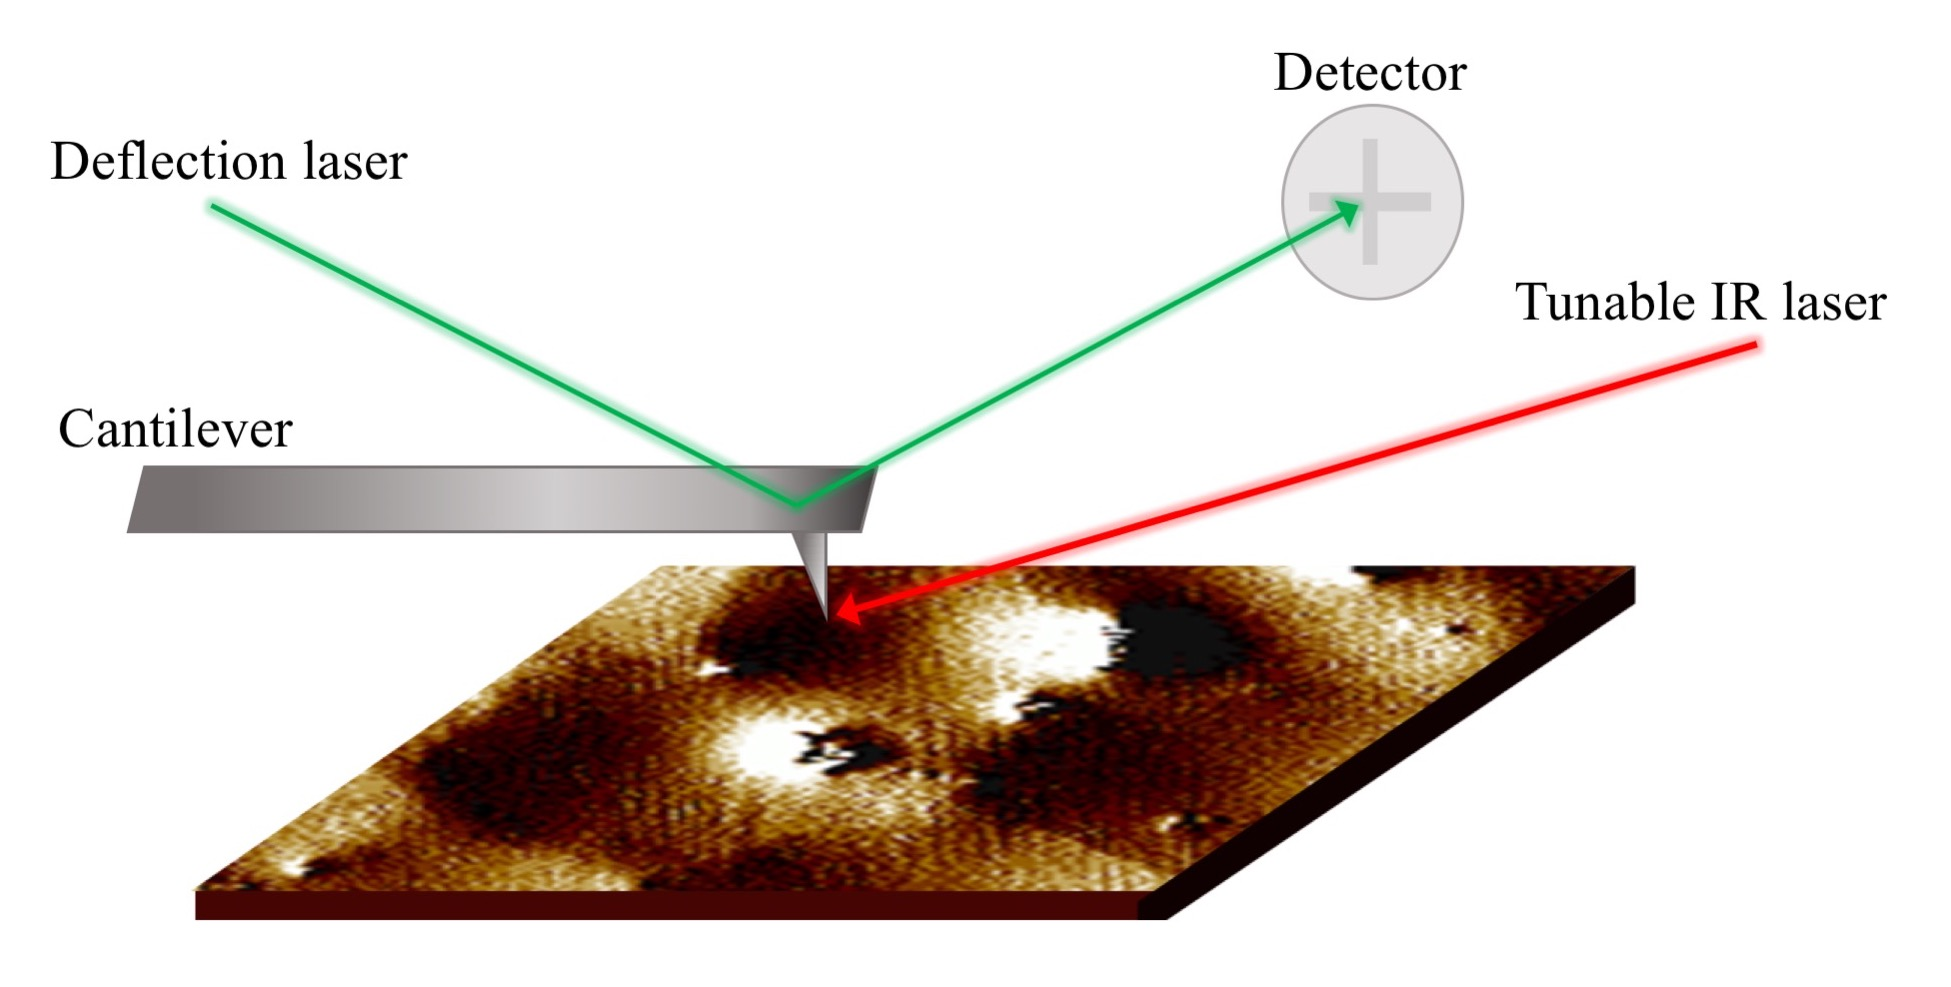
\includegraphics[width=\linewidth]{afm_diagram}
\caption[Diagram of AFM-IR schematic showing a top-down illumination system.]{Diagram of AFM-IR schematic showing a top-down illumination system. The incident inrared beam causes the sample to expand and move the probe-cantilever system. The cantilever deflection is recorded and detected by another laser beam reflected into a photodiode detector.~\autocite{Morsch,dazzi2017}}
\label{fig:afm_diagram}
\end{figure}

AFM-IR spectra are directly comparable to conventional IR spectra because the oscillations of the cantilever are proportional to the absorption coefficient of the sample. This means that peak locations and band shapes will not be affected by the collection method, and samples can be studied using both methods concurrently.~\autocite{dazzi2017,kurouski} It is possible to collect either at one point on the sample over all frequencies, generating a spectrum, or over all points on the sample at a single frequency, generating a map of the intensity at that frequency. 

\subsection[Scanning electron microscopy]{Scanning electron microscopy}
\label{subsection1.2.2}

 \todo{Needs writing.}




%!TEX root = ../thesis.tex
%*******************************************************************************
%****************************** Second Chapter *********************************
%*******************************************************************************

\chapter{Experimental}

\ifpdf
    \graphicspath{{Chapter2/Figs/Raster/}{Chapter2/Figs/PDF/}{Chapter2/Figs/}}
\else
    \graphicspath{{Chapter2/Figs/Vector/}{Chapter2/Figs/}}
\fi


\section[Preparation of samples]{Preparation of pigment samples}
\label{section2.1}

Reference samples were acquired from Dr. Spike Bucklow from the Hamilton Kerr Institute collection and Dr. Andrea Kirkham from her sample library. All reference samples were loose powder and are described qualitatively in Table \ref{table:ref_sample}. Samples are pictured in storage in \textit{Figures \ref{fig:sample_bags}} and \textit{\ref{fig:sample_vials}}, and pressed on slides for confocal Raman analysis in \textit{Figure \ref{fig:sample_slides}}.

Prior to Raman analysis, small quantities of each pigment were pressed onto double-sided sellotape and smoothed using a metal spatula. Prior to SEM-EDS analysis, small quantities of each pigment were pressed onto high purity conductive double-sided adhesive carbon tabs to minimise surface charging.

\begin{table}[H]
\caption{Reference sample descriptions}
\centering
\label{table:ref_sample}
\begin{tabular}{c c}
\toprule
Reference sample & Qualitative physical description \\
\midrule
HKI natural azurite & Natural azurite, medium sandy blue \\
HKI cross section & Natural and artifical azurite \\
KE 1a, KE 1b & Green bice, light pale teal green \\
KE 2 & Green verditer, CuCO\textsubscript{3} $\cdot$ Cu(OH)\textsubscript{2}, bright teal green \\
KE 3 & Light verditer bice, medium dark blue \\
KE 4 & Blue bice, medium grey blue \\
KE 5 & Blue verditer, 2CuCO\textsubscript{3} $\cdot$ Cu(OH)\textsubscript{2}, dark blue \\
Fitz 1 & Blue verditer, Fitzpatrick 10180, dark blue \\
Az 1 & Azurite, medium light blue \\
Az 2 & Azurite, dark deep blue \\
Az Op & Azurite, medium blue \\
Az Mag & Azurite, medium teal blue \\
Ma 1 & Malachite, medium light green \\
\bottomrule
\end{tabular}
\end{table}

\begin{figure}[H]
\centering
  \includegraphics[width=0.75\linewidth]{sample_bags}
\caption[Samples KE 1-5 and Fitz 1.]{Samples KE 1-5 and Fitz 1 shown in storage bags.}
\label{fig:sample_bags}
\end{figure}

\begin{figure}[H]
\centering
  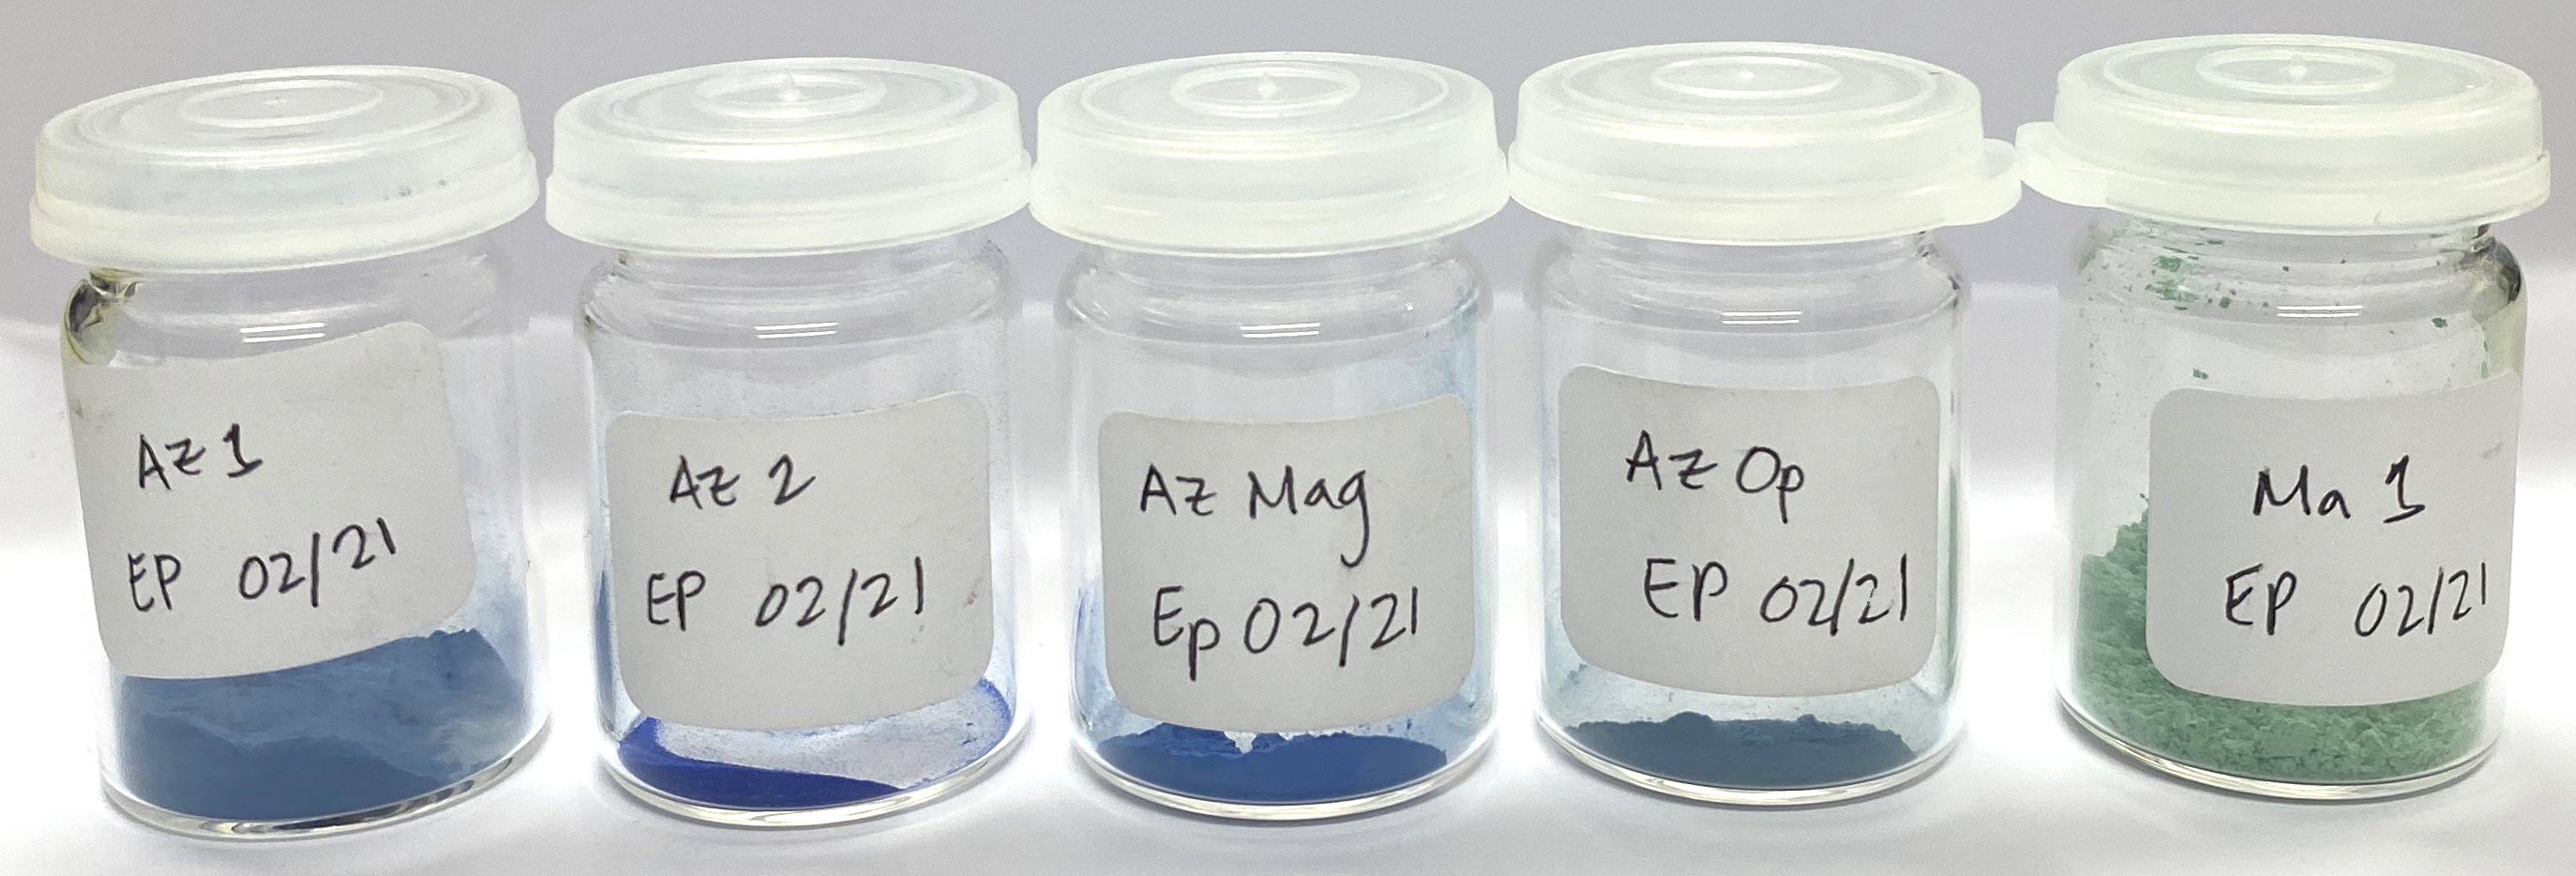
\includegraphics[width=0.75\linewidth]{sample_vials}
\caption[Samples Az 1, Az 2, Az Op, Az Mag, and Ma 1.]{Samples Az 1, Az 2, Az Op, Az Mag, and Ma 1, shown in small sample vials.}
\label{fig:sample_vials}
\end{figure}

\begin{figure}[H]
\centering
  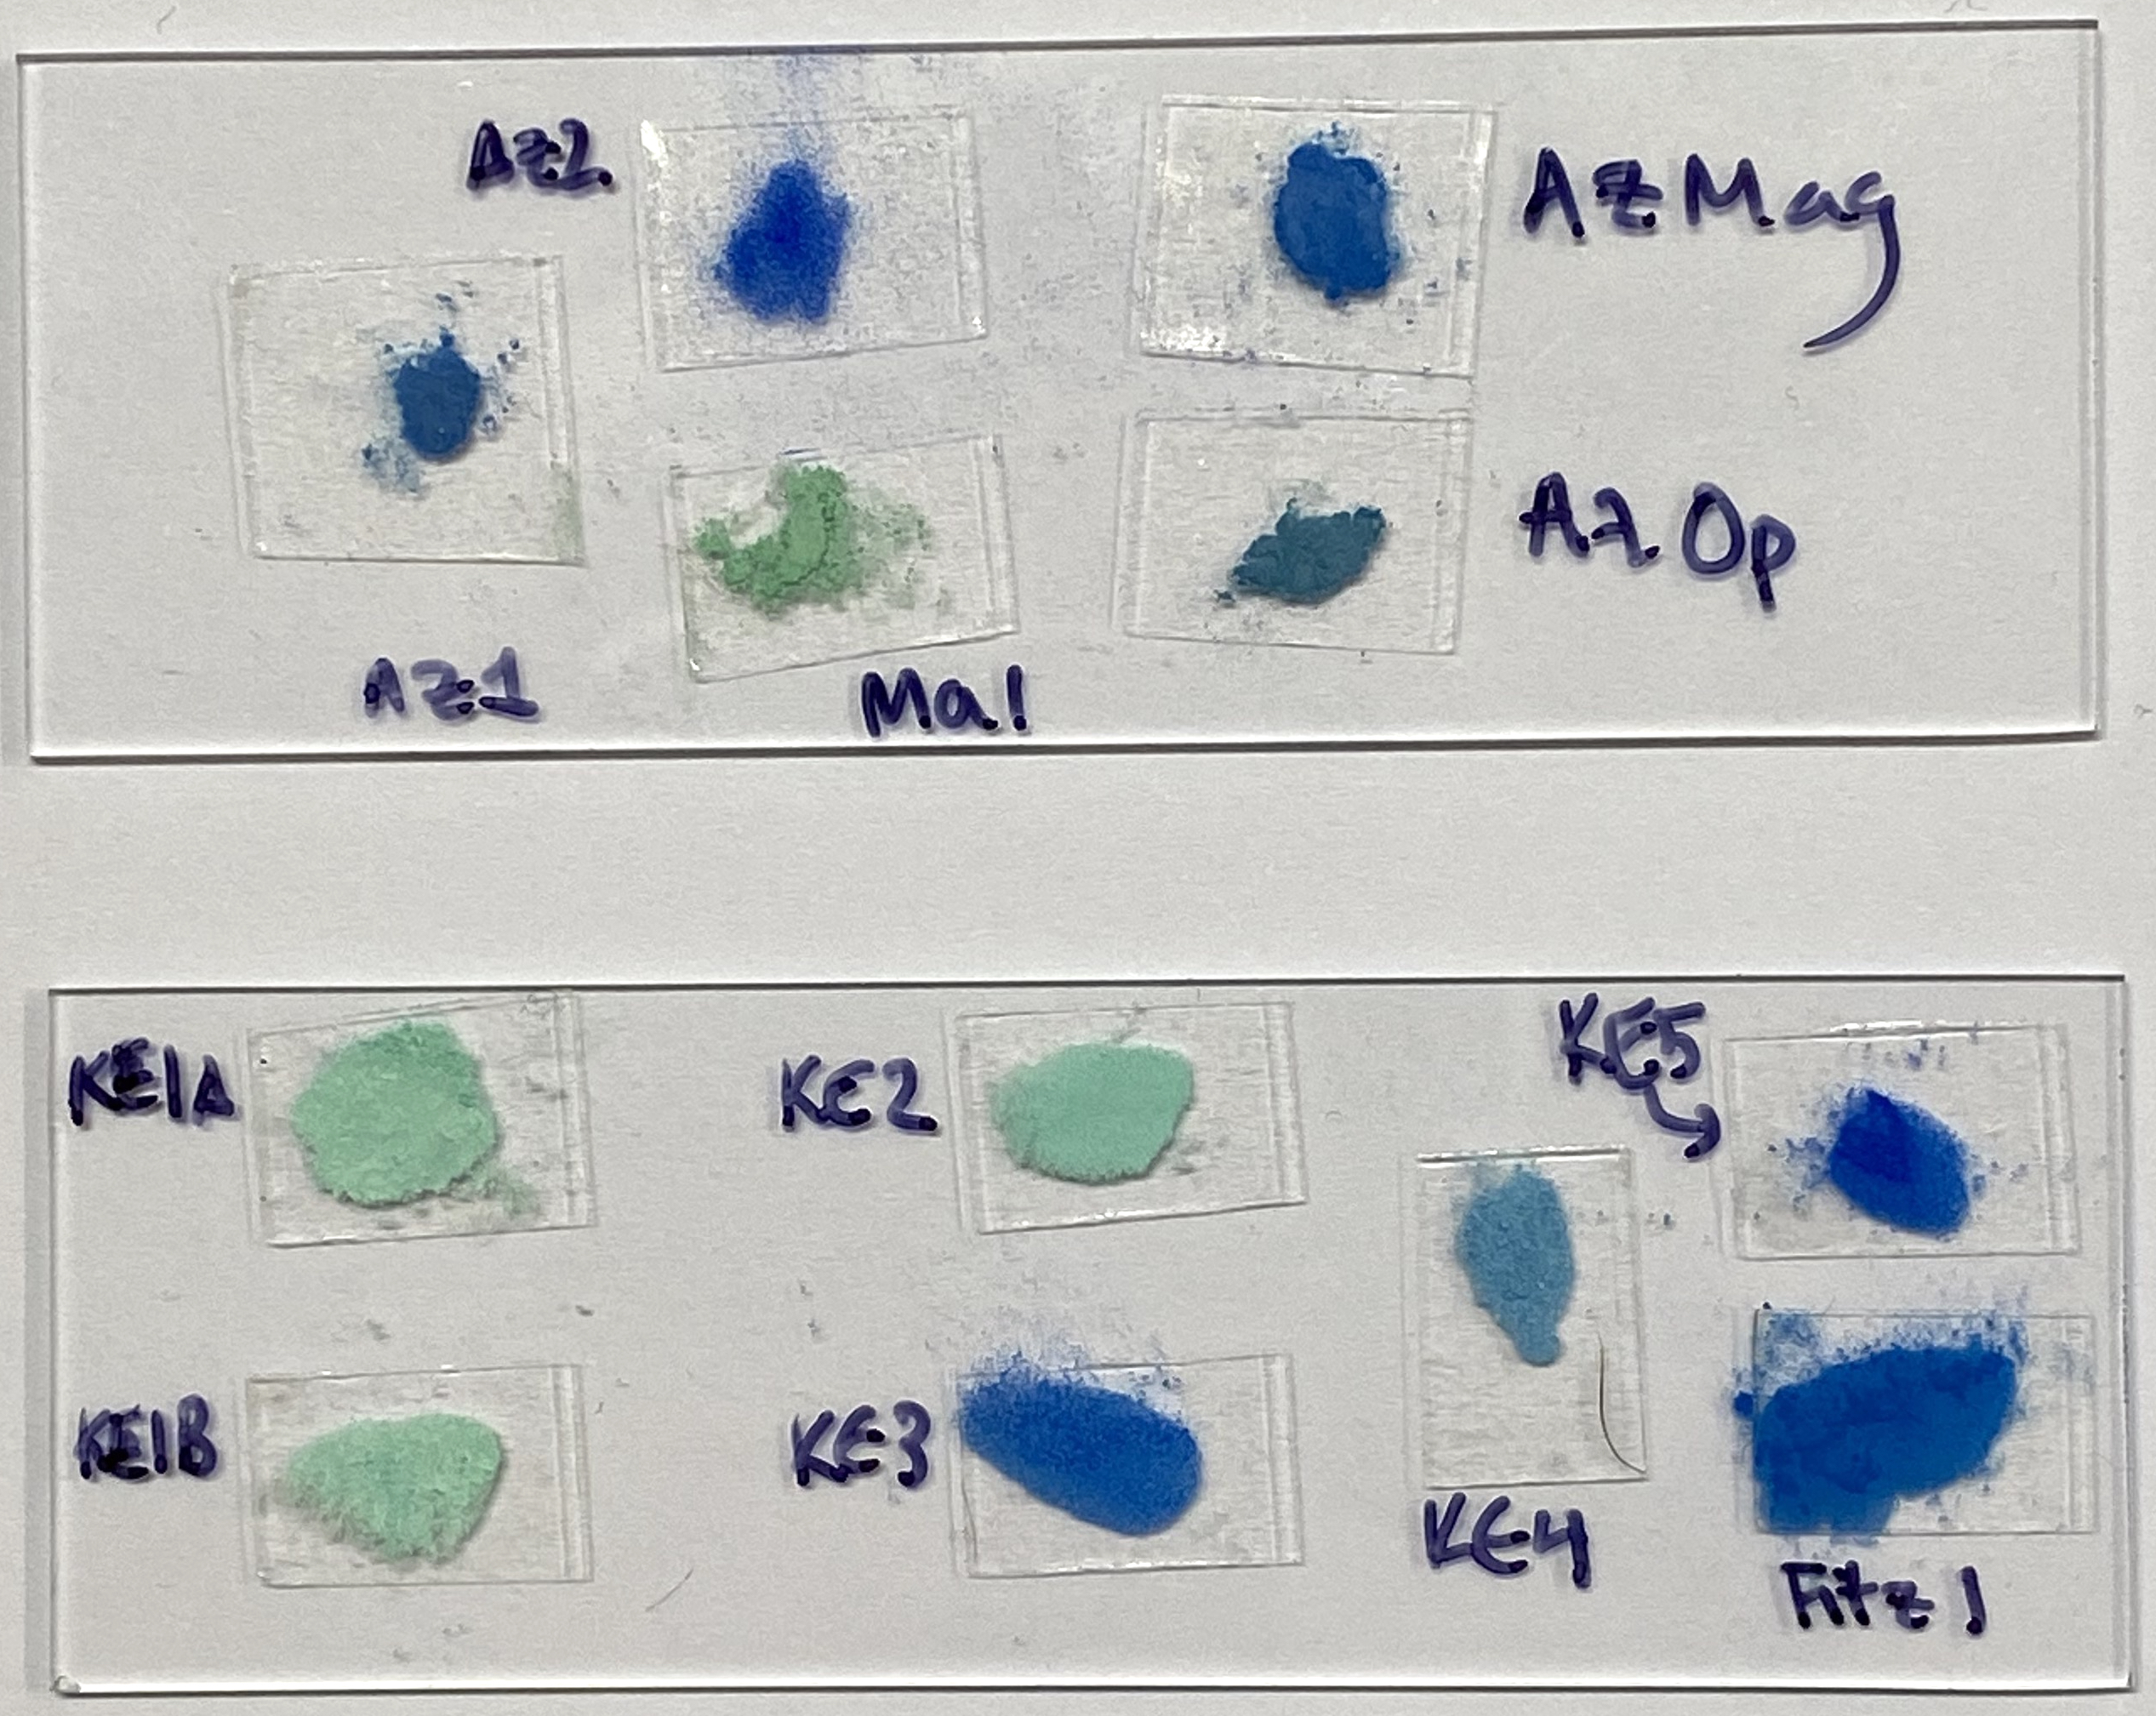
\includegraphics[width=0.75\linewidth]{sample_slides}
\caption[All reference samples shown pressed on double-sided tape and prepared for Raman analysis.]{All reference samples shown pressed on double-sided tape and prepared for Raman analysis.}
\label{fig:sample_slides}
\end{figure}

Pigment samples were also embedded in resin and polished to create a flat, uniform surface for Raman mapping and AFM analysis. A small quantity of pigment was placed in a coin shaped mold and a clear polyester resin (Tiranti clear casting resin) was poured over the pigment. The resin was allowed to set for 48 hours before being removed from the mold. Samples were filed to approximately 5 mm in height and the pigment containing surface was polished using three sequential grit sizes of silicon carbide paper (English Abrasives) and polishing cloth (Buehler), using a fine grade cerium oxide polishing powder (Beckman-RIIC) in ethanol. Finally, polished samples were cleaned with ethanol to remove extra polish and debris prior to analysis.

\section[Analysis of pigment particles by Raman spectroscopy]{Analysis of pigment particles by Raman spectroscopy}
\label{section2.2}

Collection of Raman spectra of pigment samples was done using a Horiba LabRAM HR Evolution confocal Raman spectrometer with a 50x microscope objective (Olympus LMPLFLN), a 600 grooves/mm grating, and a CCD array (1024x1024 pixels). The pinhole size was 100 $\mu$m. An laser with excitation wavelength of 532 nm (diode-pumped solid-state, Laser Quantum) was selected based on optimal signal to noise ratio with lack of sample damage. We expect that the samples under consideration in this study, azurite and malachite, will show strong signals at 532 nm based on previous work on these materials.~\autocite{Bicchieri} Two other excitation wavelengths, 633 nm and 785 nm, were also tested and found to give inferior results at longer acquisition times and/or higher laser powers at the sample surface (\textit{Figure \ref{fig:Az1_wavelength_comparison}}. Spectra were collected in the confocal mode focusing on specific pigment grains.

\begin{figure}[H]
\centering
  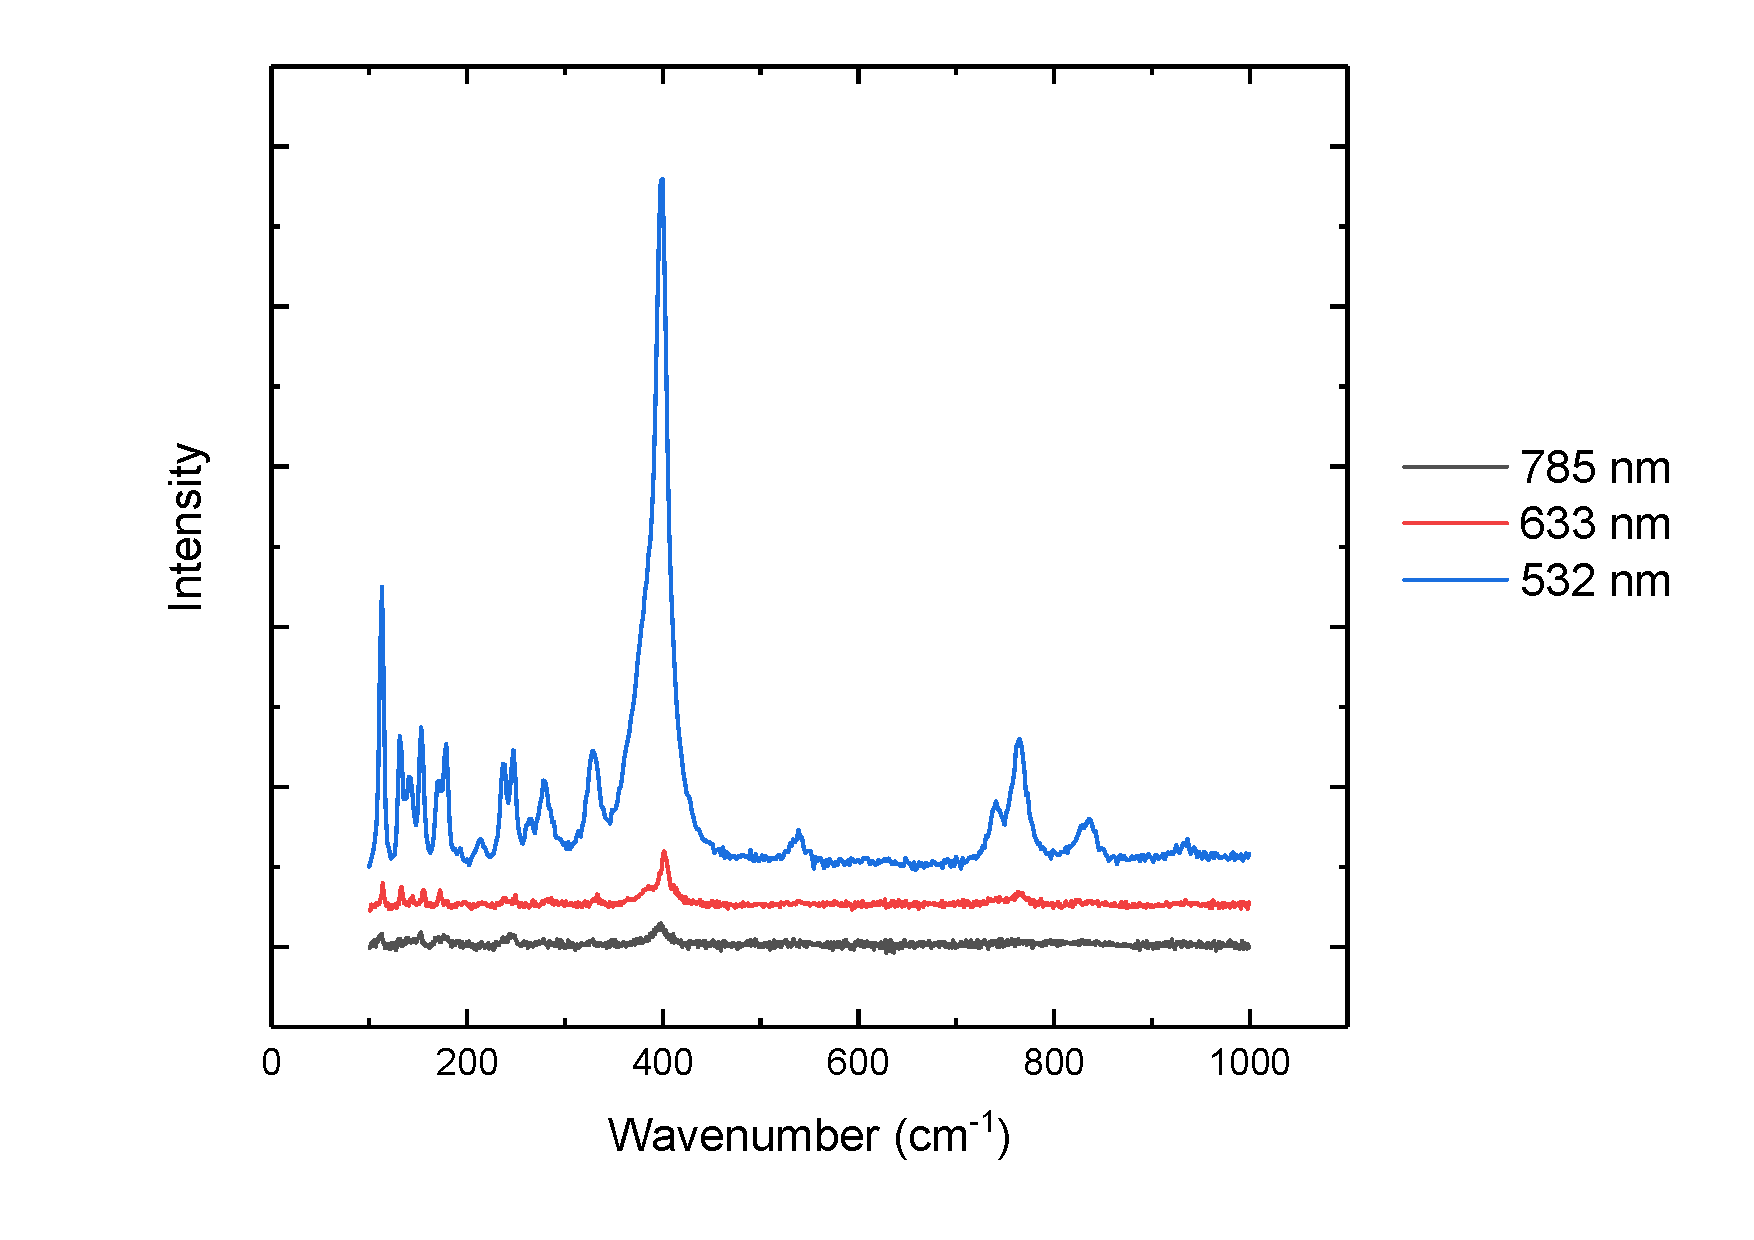
\includegraphics[width=0.75\linewidth]{Az1_wavelength_comparison}
\caption[Comparison of spectra collected at 532, 633, and 785 nm excitation wavelengths from sample Az 1.]{Comparison of spectra collected at 532 (blue), 633 (red), and 785 nm (black) excitation wavelengths from sample Az 1.}
\label{fig:Az1_wavelength_comparison}
\end{figure}

Optimal collection parameters were determined to maximise the signal to noise ratio of spectra while avoiding sample damage and minimising collection times (\textit{Figure \ref{fig:Az1_laserpower_comp_532}}). The damage threshold of pigment grains was observed to depend on the sample identity and the size of the grain sampled. This has been observed in previous studies and is expected.~\autocite{Cardell,Mattei} Damage to azurite (blue bice, blue verditer) samples was observed to occur at 50\% power or XXXX mW with an acquisition time of 10 s and 10 accumulations. Malachite (green verditer) has a lower damage threshold, occurring at at 25\% power or XXXX mW with an acquisition time of 10 s and 10 accumulations. 10\% power or XXXX mW with an acquisition time of 10 s and 10 accumulations did not cause observable damage to any reference sample. For the sake of consistency, this lower surface power and acquisition time was selected for all samples as it gave a satisfactory signal quality. 

\begin{figure}[H]
\centering
  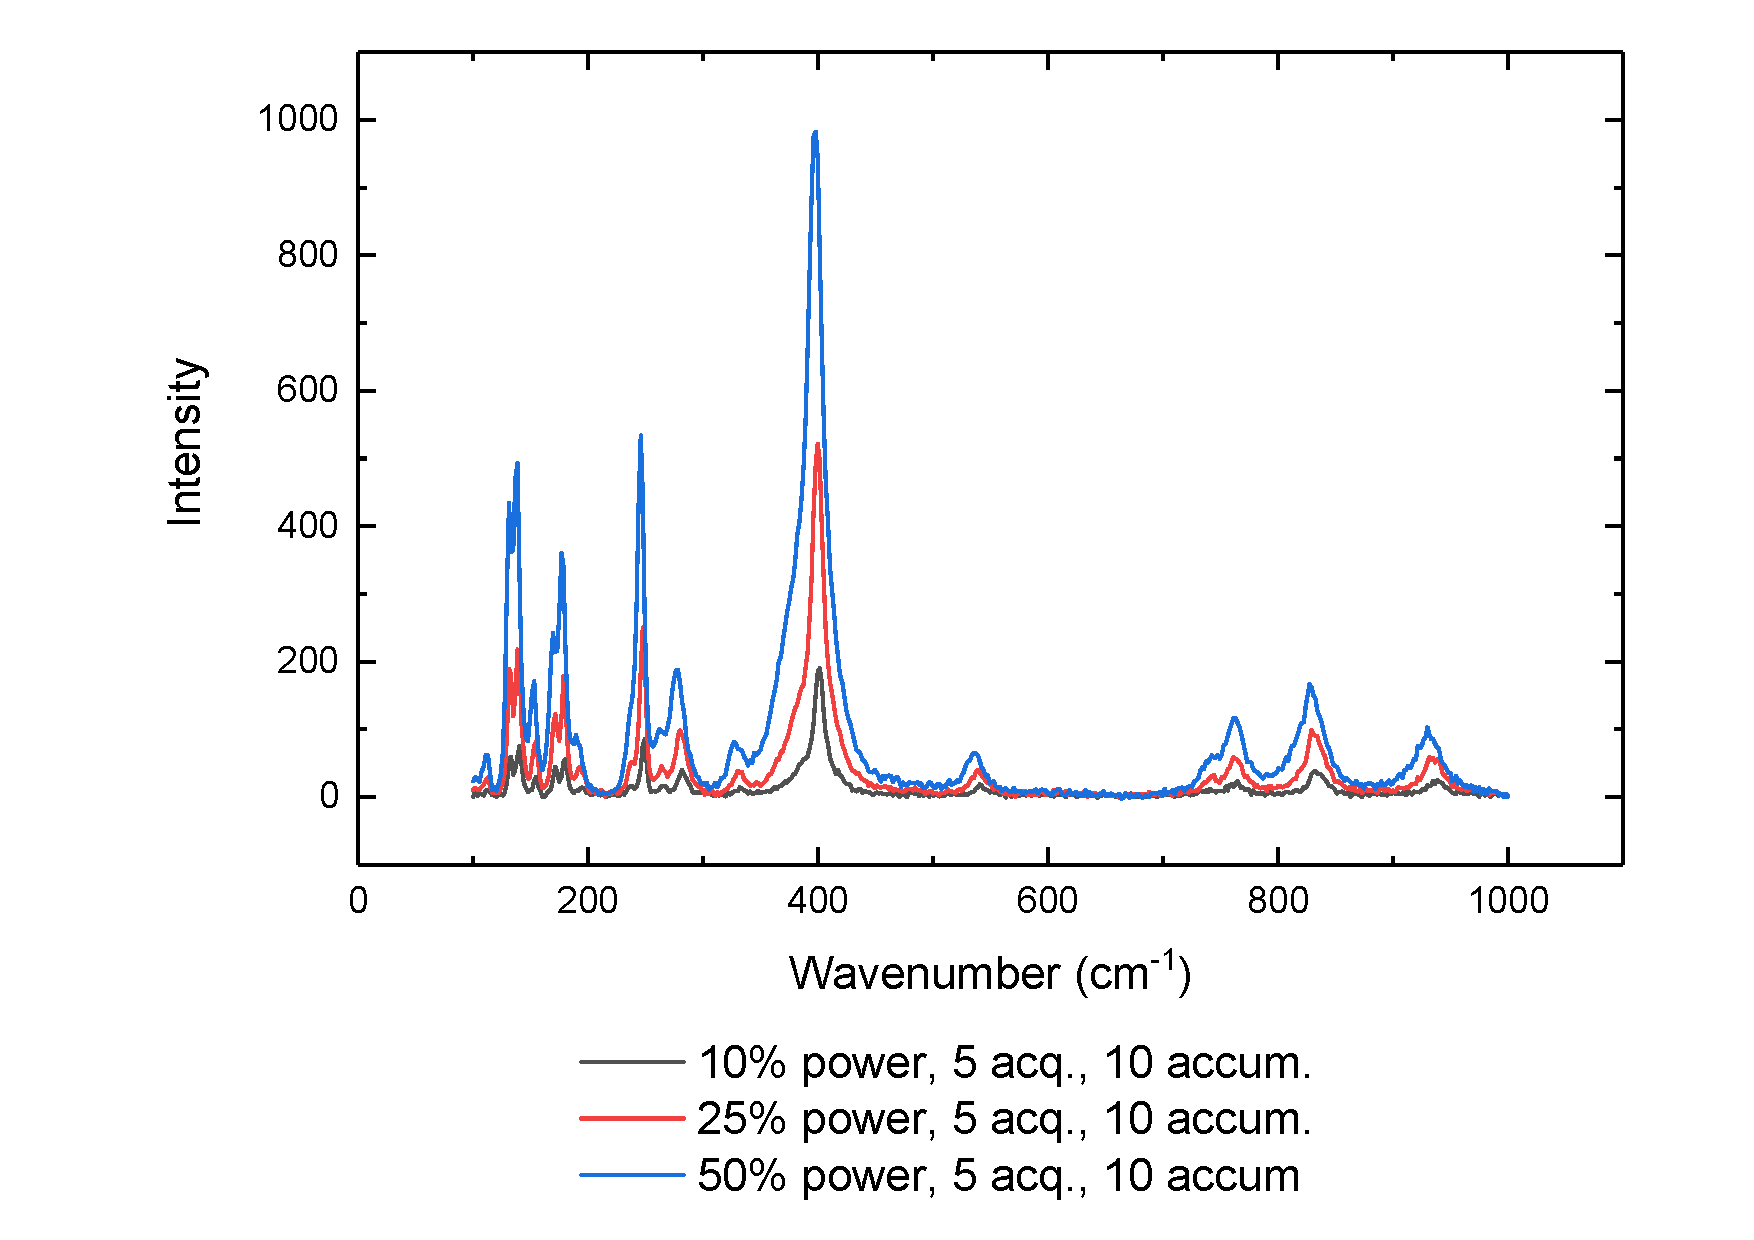
\includegraphics[width=0.75\linewidth]{Az1_laserpower_comp_532}
\caption[Comparison of spectra collected using 532 nm excitation wavelength at 10\%, 25\%, and 50\% power.]{Comparison of spectra collected using 532 nm excitation wavelength at 10\% (black), 25\% (red), and 50\% (blue) power (5 acquisitions, 10 accumulations).}
\label{fig:Az1_laserpower_comp_532}
\end{figure}

\todo{add specific parameters about lasers - this is not in due to the weirdness about the 532 nm laser powers currently.}

Raman spectra were processed using OriginPro 2017 software. All spectra were fit to a spline baseline. %and normalised to the peak intensity at XXXX cm\textsuperscript{-1}, selected based on \mynote{XXXX fill details in here.}

\section[Analysis of pigment particles by SEM-EDS]{Analysis of pigment particles by SEM-EDS}
\label{section2.3}

Pigment particle shape, size, and regularity, as well as elemental composition, were characterized using scanning electron microscopy (SEM) coupled to energy dispersive X-ray spectroscopy (EDS). Samples were prepared as described in section \ref{section2.1}. Micrographs of pigments were collected at several magnifications rangeing from 250x to 2500x using a JEOL JSM-5510LV scanning electron microscope, imaged using the secondary electron detector. The working distance between the sample and the beam source was 20 mm. The accelerating voltage was 10 keV, which caused minimal charging on the surface of the sample, unless otherwise noted. ED spectra were collected at the same time as SEM imaging using an Oxford instruments probe (add specs) and (add type) detector and processed using XXXX software. The accelerating voltage was 10 keV unless otherwise noted, which limited detection of heavier elements but minimized surface charging. Elemental mapping using EDS was also carried out to detect variation between pigment grains within the same sample and identify local differences. 

\todo{add EDS specs}
%!TEX root = ../thesis.tex
%*******************************************************************************
%****************************** Third Chapter **********************************
%*******************************************************************************
\chapter{Data and analysis}

% **************************** Define Graphics Path **************************
\ifpdf
    \graphicspath{{Chapter3/Figs/Raster/}{Chapter3/Figs/PDF/}{Chapter3/Figs/}}
\else
    \graphicspath{{Chapter3/Figs/Vector/}{Chapter3/Figs/}}
\fi

\section[SEM Data]{SEM Data}
\label{section3.1}

\subsection[Azurite and blue verditer]{Azurite and blue verditer}
\label{subsection3.1.1}

This section discusses qualitatively the morphological features, regularity, and approximate particle size of the reference samples described in \textit{Table \ref{table:ref_sample}}.  
% ************************************************     HKI nat az sample     *******************************************************************

\textit{Figures \ref{fig:hki_nat_az_sem_1}-\ref{fig:hki_nat_az_sem_5}} show the sample HKI natural azurite. This sample is of unknown date and provenance but is confirmed to be naturally produced, which offers a baseline against which to compare other samples known to be synthetic or of unknown origin. Maginification ranges from 250x to 4000x. Significant surface charging was not observed with this sample.

In \textit{Figure \ref{fig:hki_nat_az_sem_1}}, two areas are shown at 250x magnification. Particle sizes are very irregular, as are shapes and volumes. Particles appear to be relatively flat-sided rather than rough. 

\begin{figure}[H]
\centering
\begin{minipage}{.45\textwidth}
  \centering
  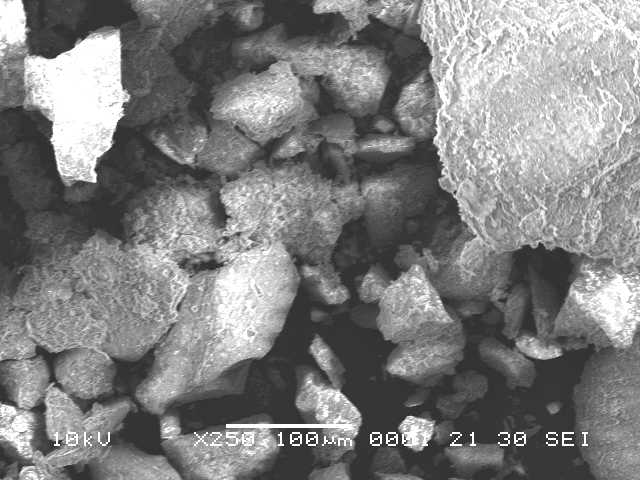
\includegraphics[width=\linewidth]{HKI_natural_azurite_x250_3_040521}
\end{minipage}
\begin{minipage}{.45\textwidth}
  \centering
  \includegraphics[width=\linewidth]{HKI_natural_azurite_x250_5_040521}
\end{minipage}
\caption[SEM images: Sample HKI, natural azurite]{SEM images: Sample HKI, natural azurite. Magnification: 250x.}
\label{fig:hki_nat_az_sem_1}
\end{figure}

It is possible to see the surface texture of larger particles more clearly at 750x magnification in \textit{Figure \ref{fig:hki_nat_az_sem_2}}. It appears that there are smaller particles embedded in or settled on the surface of larger particles, making a rough surface. Particles have clearly sharp angular edges and are not rounded. At this magnification the large variation in particle size is apparent, and the asymmetry of the material is noted.

\begin{figure}[H]
\centering
\begin{minipage}{.45\textwidth}
  \centering
  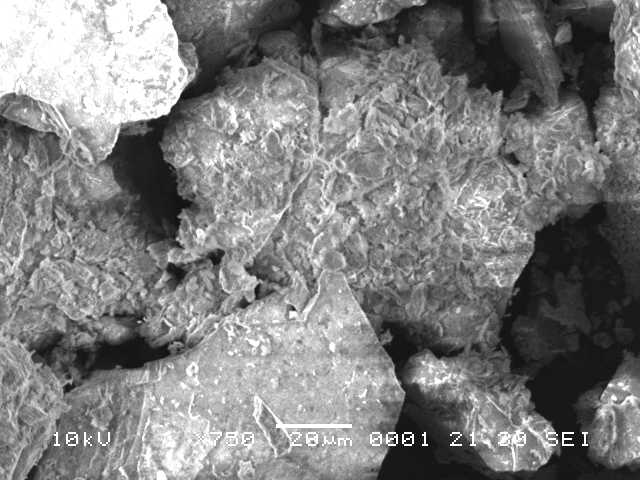
\includegraphics[width=\linewidth]{HKI_natural_azurite_x750_1_040521}
\end{minipage}
\begin{minipage}{.45\textwidth}
  \centering
  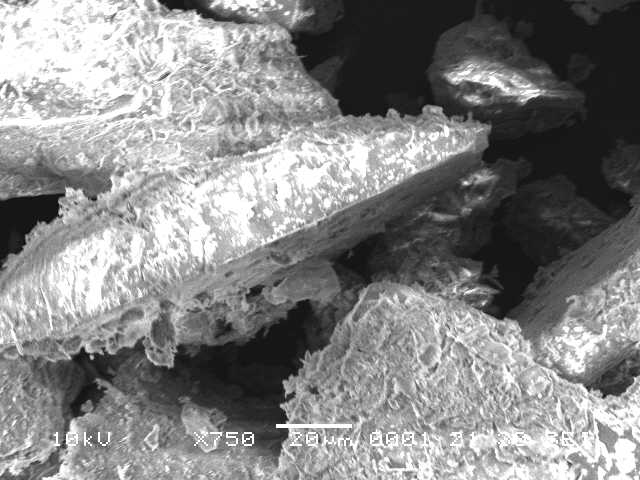
\includegraphics[width=\linewidth]{HKI_natural_azurite_x750_3_040521}
\end{minipage}
\caption[SEM images: Sample HKI, natural azurite]{SEM images: Sample HKI, natural azurite. Magnification: 750x.}
\label{fig:hki_nat_az_sem_2}
\end{figure}

The fine surface detail on the flat sides of larger particles can be observed at 1500x magnification in \textit{Figure \ref{fig:hki_nat_az_sem_3}}. The image on the right shows several more spherical looking particles, though many more appear asymmetrical with uneven sharp edges. The size of the texture on the surface is consistent in size in contrast to the macro size heterogeneity.

\begin{figure}[H]
\centering
\begin{minipage}{.45\textwidth}
  \centering
  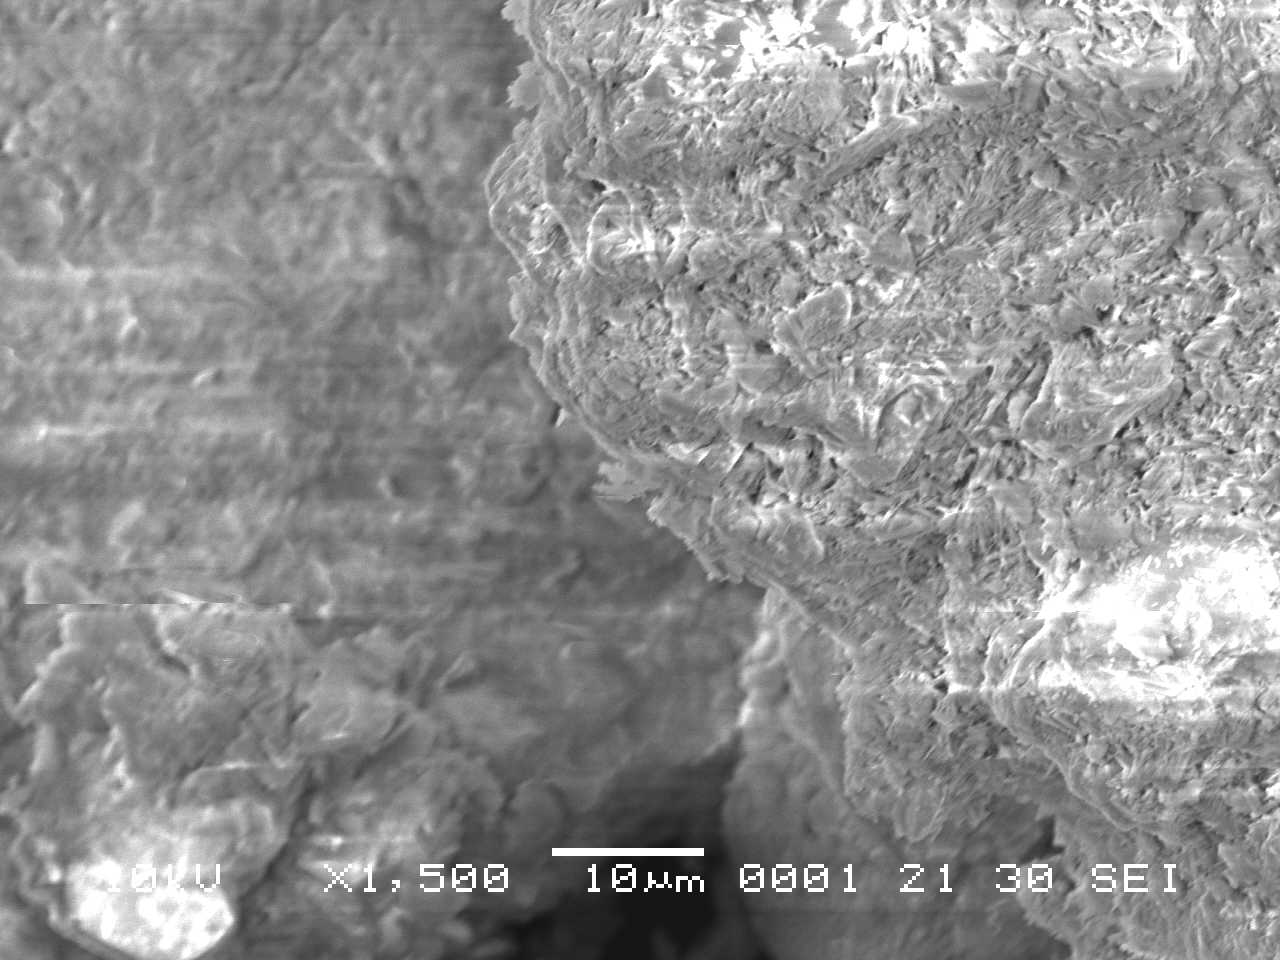
\includegraphics[width=\linewidth]{HKI_natural_azurite_x1500_2_040521}
\end{minipage}
\begin{minipage}{.45\textwidth}
  \centering
  \includegraphics[width=\linewidth]{HKI_natural_azurite_x1500_4_040521}
\end{minipage}
\caption[SEM images: Sample HKI, natural azurite]{SEM images: Sample HKI, natural azurite. Magnification: 1500x.}
\label{fig:hki_nat_az_sem_3}
\end{figure}

\textit{Figure \ref{fig:hki_nat_az_sem_4}} shows two images at 2000x magnification. The image on the right shows clear sharp-sided particles. These are extremely uneven. The left image, on the other hand, shows flat irregular small particles layered over one another like flakes.

\begin{figure}[H]
\centering
\begin{minipage}{.45\textwidth}
  \centering
  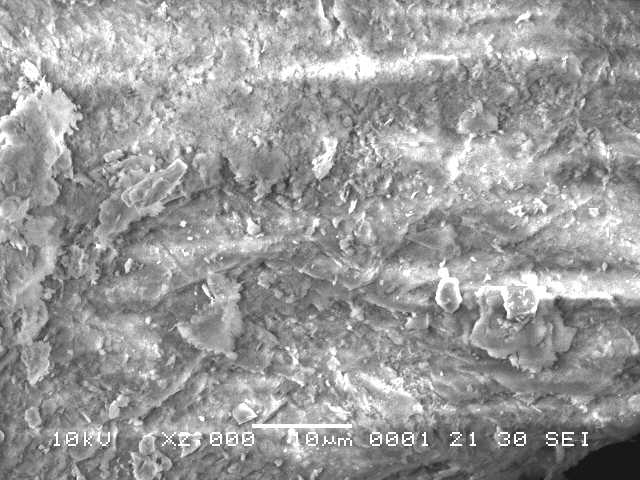
\includegraphics[width=\linewidth]{HKI_natural_azurite_x2000_1_040521}
\end{minipage}
\begin{minipage}{.45\textwidth}
  \centering
  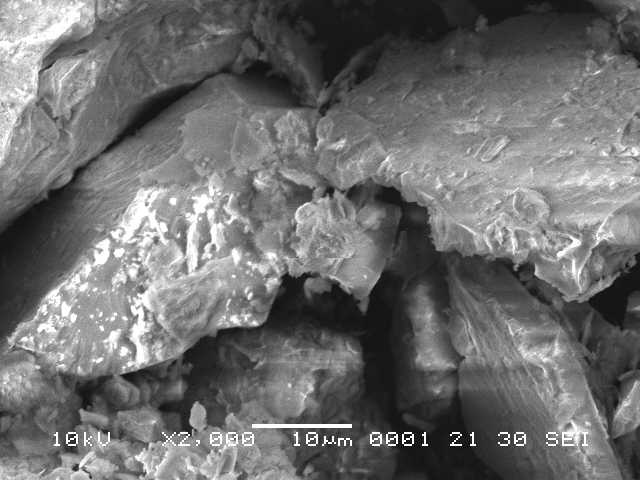
\includegraphics[width=\linewidth]{HKI_natural_azurite_x2000_3_040521}
\end{minipage}
\caption[SEM images: Sample HKI, natural azurite]{SEM images: Sample HKI, natural azurite. Magnification: 2000x.}
\label{fig:hki_nat_az_sem_4}
\end{figure}

At very high magnification (4000x), \textit{Figure \ref{fig:hki_nat_az_sem_5}} shows the fine structure of the sample very clearly. There is still significant size variation at this magnification, and interesting needle like crystal formations are observed. These do appear to be orientated in some places, possibly showing the areas of crystal nucleation and growth. Other needle like crystals appear randomly orientated. Notably, this ordering is not readily observed in other samples, though needle like crystals are.

\begin{figure}[H]
\centering
\begin{minipage}{.45\textwidth}
  \centering
  \includegraphics[width=\linewidth]{HKI_natural_azurite_x4000_2_040521}
\end{minipage}
\begin{minipage}{.45\textwidth}
  \centering
  \includegraphics[width=\linewidth]{HKI_natural_azurite_x4000_5_040521}
\end{minipage}
\caption[SEM images: Sample HKI, natural azurite]{SEM images: Sample HKI, natural azurite. Magnification: 4000x.}
\label{fig:hki_nat_az_sem_5}
\end{figure}

% ************************************************     Az1     *******************************************************************

Sample Az1, likely from a natural source, is shown in \textit{Figures \ref{fig:az1_sem_1}} and \textit{\ref{fig:az1_sem_2}}. 

\textit{Figure \ref{fig:az1_sem_1}}, at 750x magnification, shows significant size variation in the sample. There are many flat, sharp particles as well as many smaller particles. It is difficult to determine whether the larger pieces of sample are aggregates of smaller particles or larger intact pieces; the surfaces of these appear almost pocked, especially in the left image.

\begin{figure}[H]
\centering
\begin{minipage}{.45\textwidth}
  \centering
  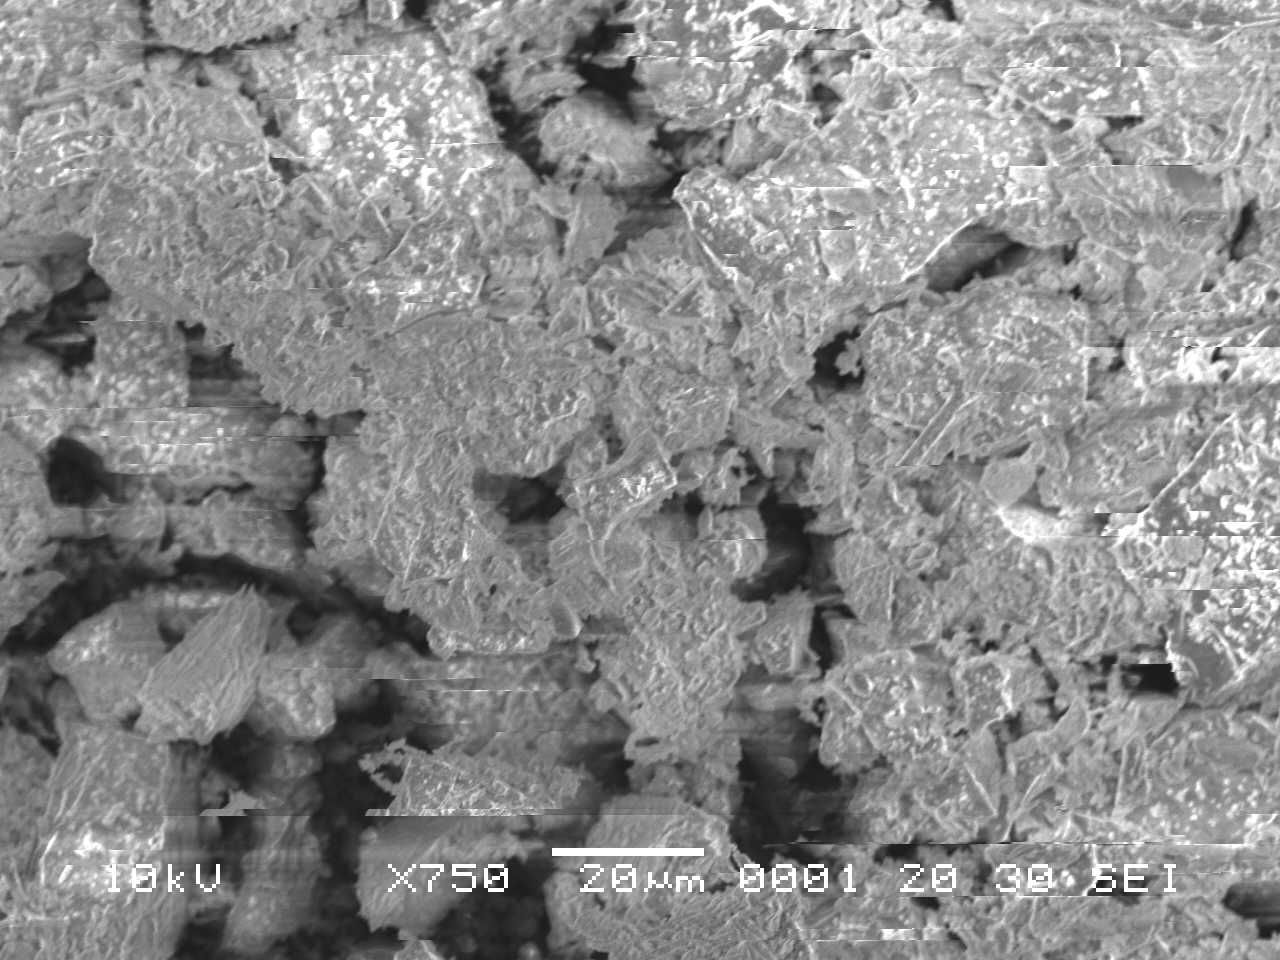
\includegraphics[width=\linewidth]{Az1_x750_3_220221}
\end{minipage}
\begin{minipage}{.45\textwidth}
  \centering
  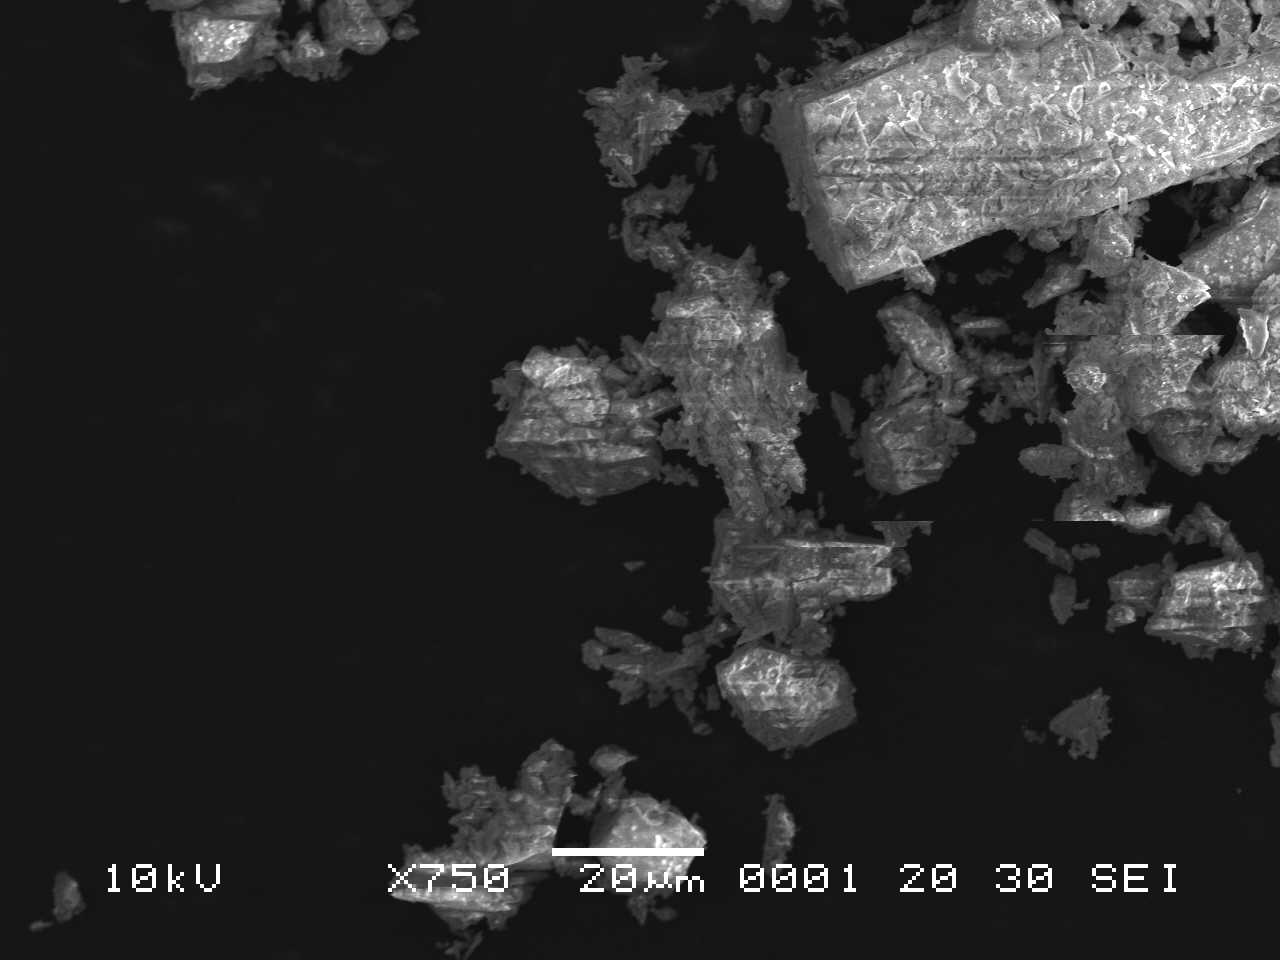
\includegraphics[width=\linewidth]{Az1_x750_6_220221}
\end{minipage}
\caption[SEM images: Sample Az1, azurite]{SEM images: Sample Az1, azurite. Magnification: 750x.}
\label{fig:az1_sem_1}
\end{figure}

\textit{Figure \ref{fig:az1_sem_2}} shows Az1 at 1500x (left) and 2000x (right). At 1500x, it is possible to observe smaller voluminous (not flat) particles on the surface of larger particles. The vast majority of pieces are irregularly shaped with choppy borders, though a few circular particles are also present. At 2000x, the image shows the flat edge of a larger particle. There is a great deal of surface texture, as well as some intriguing grid formations that do not appear to be artifacts of the SEM. These may be due to grinding and polishing of the pigment, but also may suggest some crytal ordering. Uniformity of shape and size is low at all magnifications and all over the sample.

\begin{figure}[H]
\centering
\begin{minipage}{.45\textwidth}
  \centering
  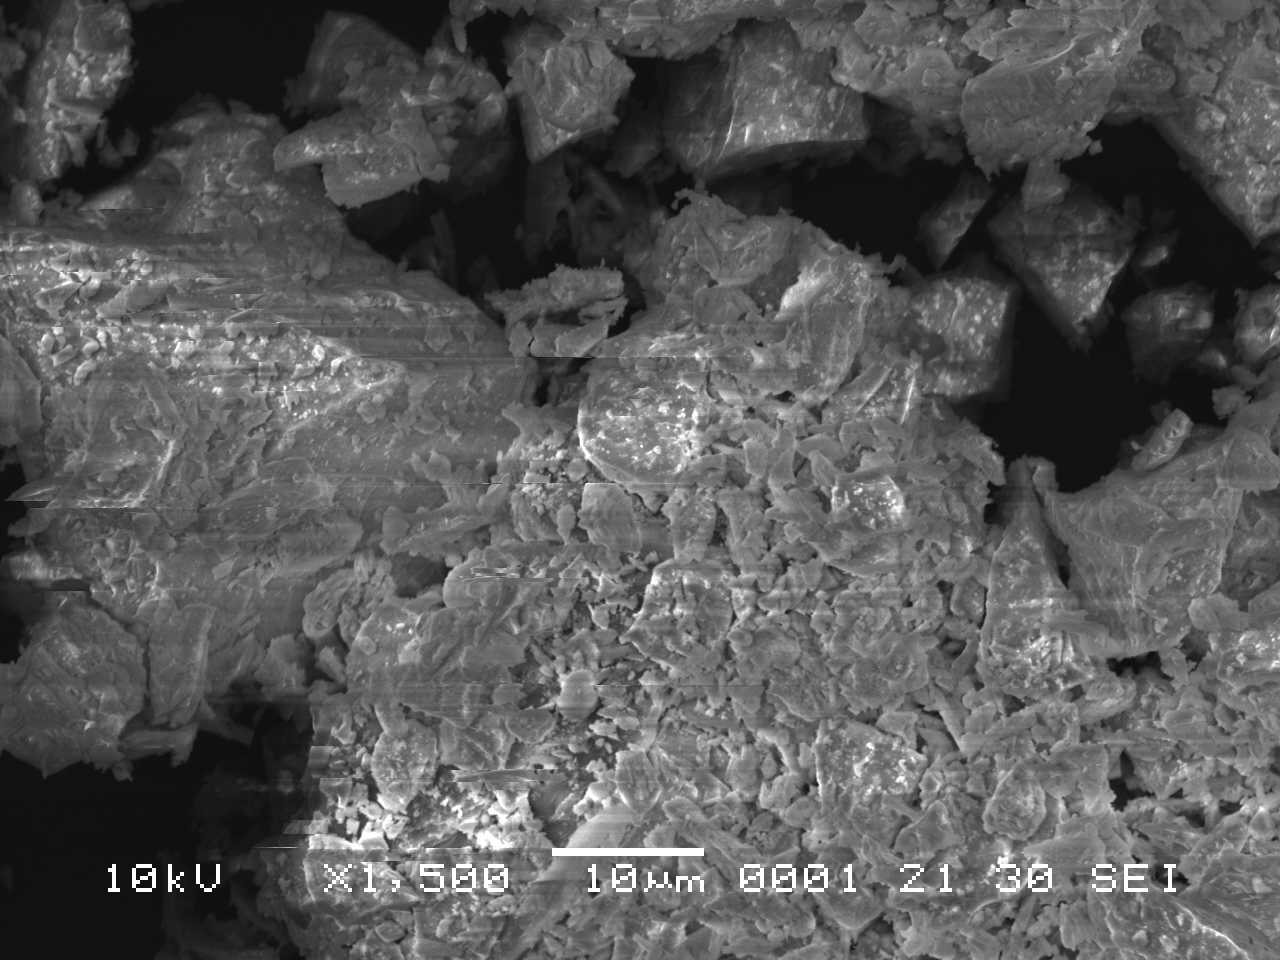
\includegraphics[width=\linewidth]{Az1_x1500_2_220221}
\end{minipage}
\begin{minipage}{.45\textwidth}
  \centering
  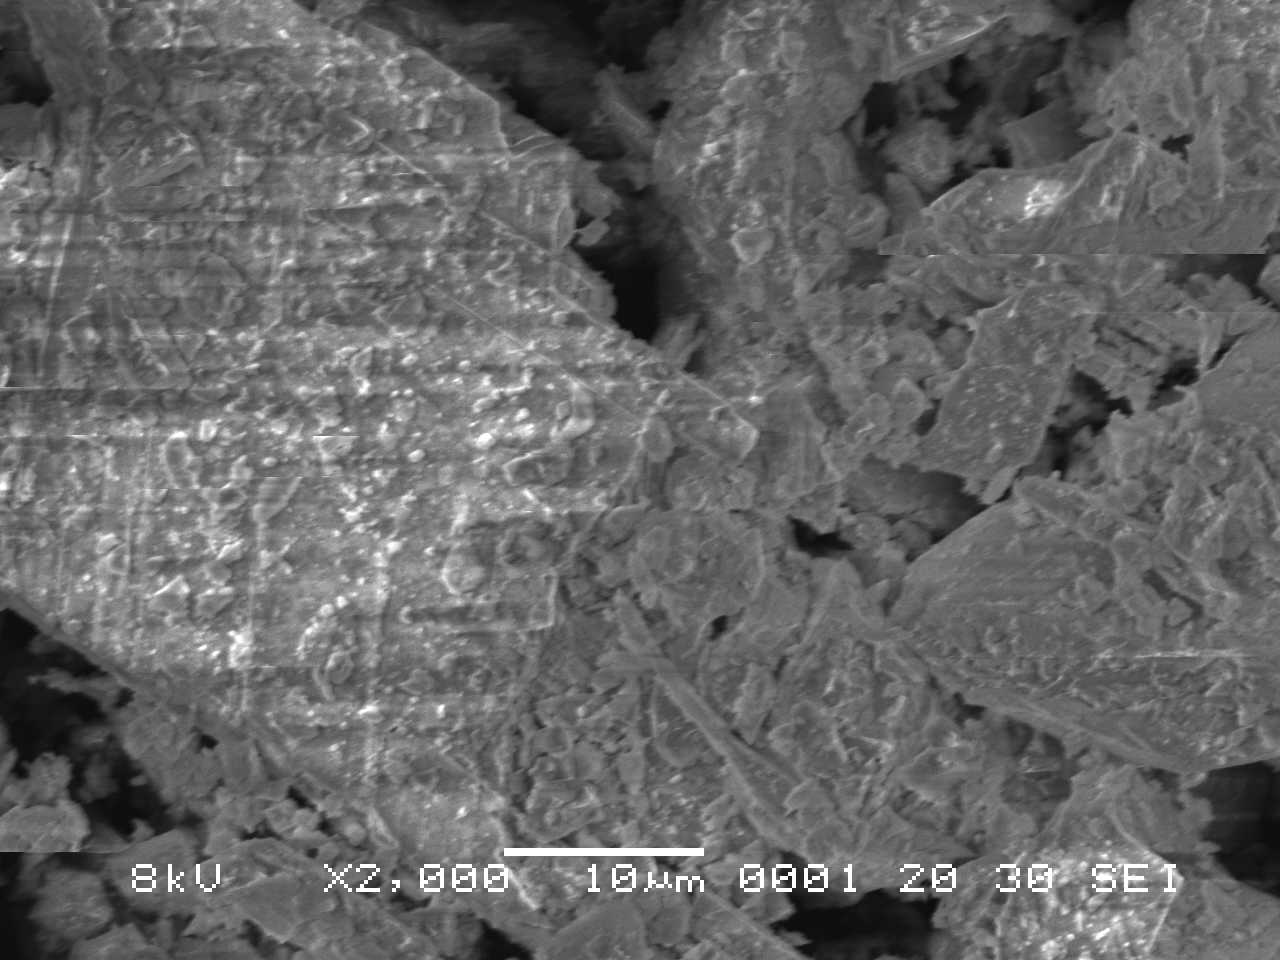
\includegraphics[width=\linewidth]{Az1_x2000_4_220221}
\end{minipage}
\caption[SEM images: Sample Az1, azurite]{SEM images: Sample Az1, azurite. Magnification: \textbf{left)} 1500x, \textbf{right)} 2000x}
\label{fig:az1_sem_2}
\end{figure}

% ************************************************     Az2     *******************************************************************

\textit{Figures \ref{fig:az2_sem_1}} and \textit{\ref{fig:az2_sem_2}} show sample Az2, which is morphologically significantly different from all other observed samples and lacks the features that appear to correlate with either natural or artificial pigment sources. Surface charging made it difficult to image this sample, and this issue was also not observed with most other samples.

In \textit{Figure \ref{fig:az2_sem_1}}, two images of the sample at 200x magnification are shown. It is interesting that although the shape of each sample is quite asymmetric and angular, the size and irregular shape is quite consistent between particules. At this magnification, the surface of the particles appears flat and smooth. It is also significant that these particles are much larger than the average particle size observed in other samples, which may suggest industrial pigment grinding. Otherwise, this consistency could also reflect a synthetic origin, with controlled conditions of crystal growth.

\begin{figure}[H]
\centering
\begin{minipage}{.45\textwidth}
  \centering
  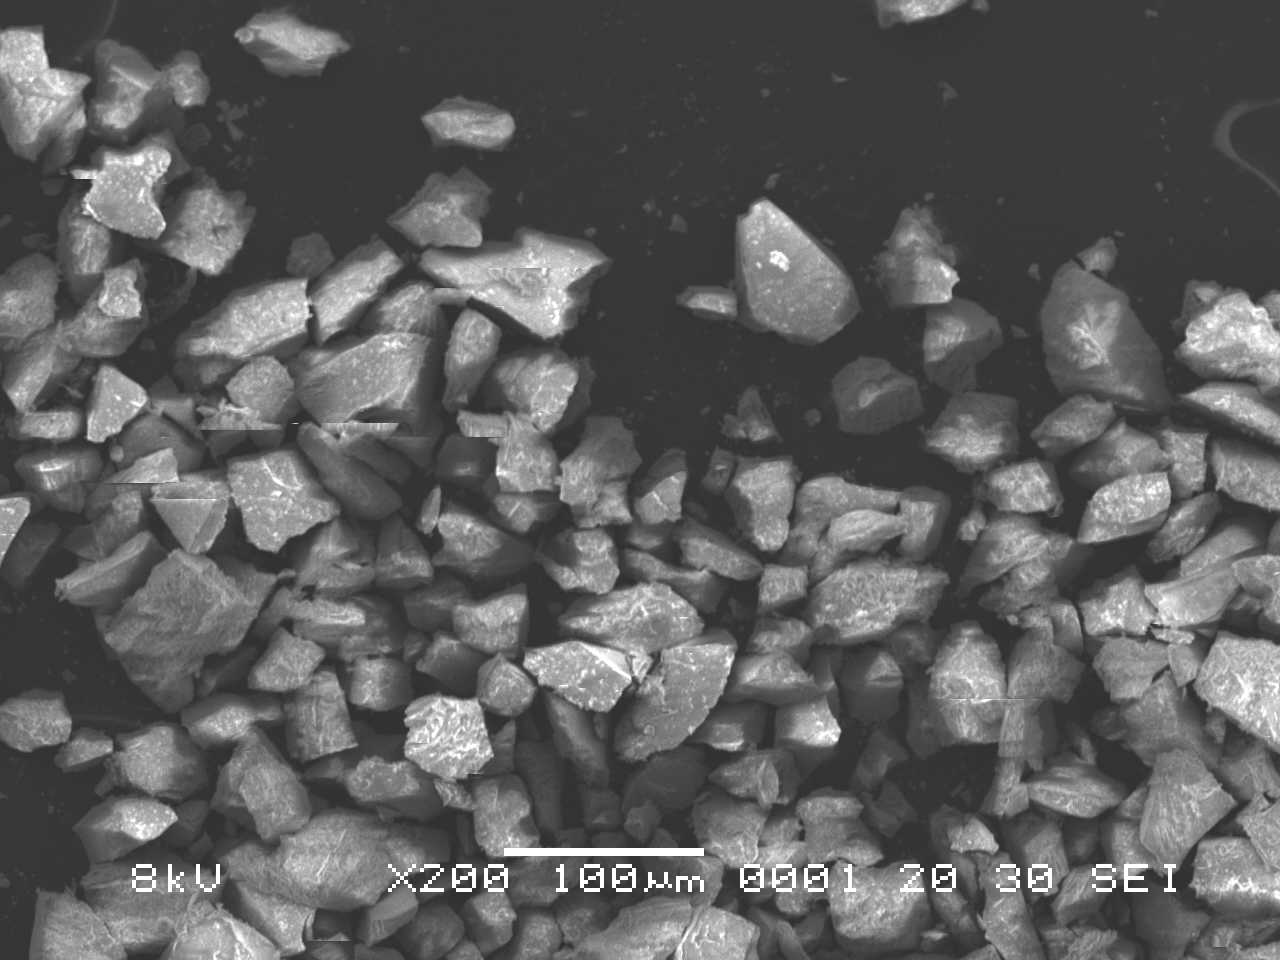
\includegraphics[width=\linewidth]{Az2_x200_1_240221}
\end{minipage}
\begin{minipage}{.45\textwidth}
  \centering
  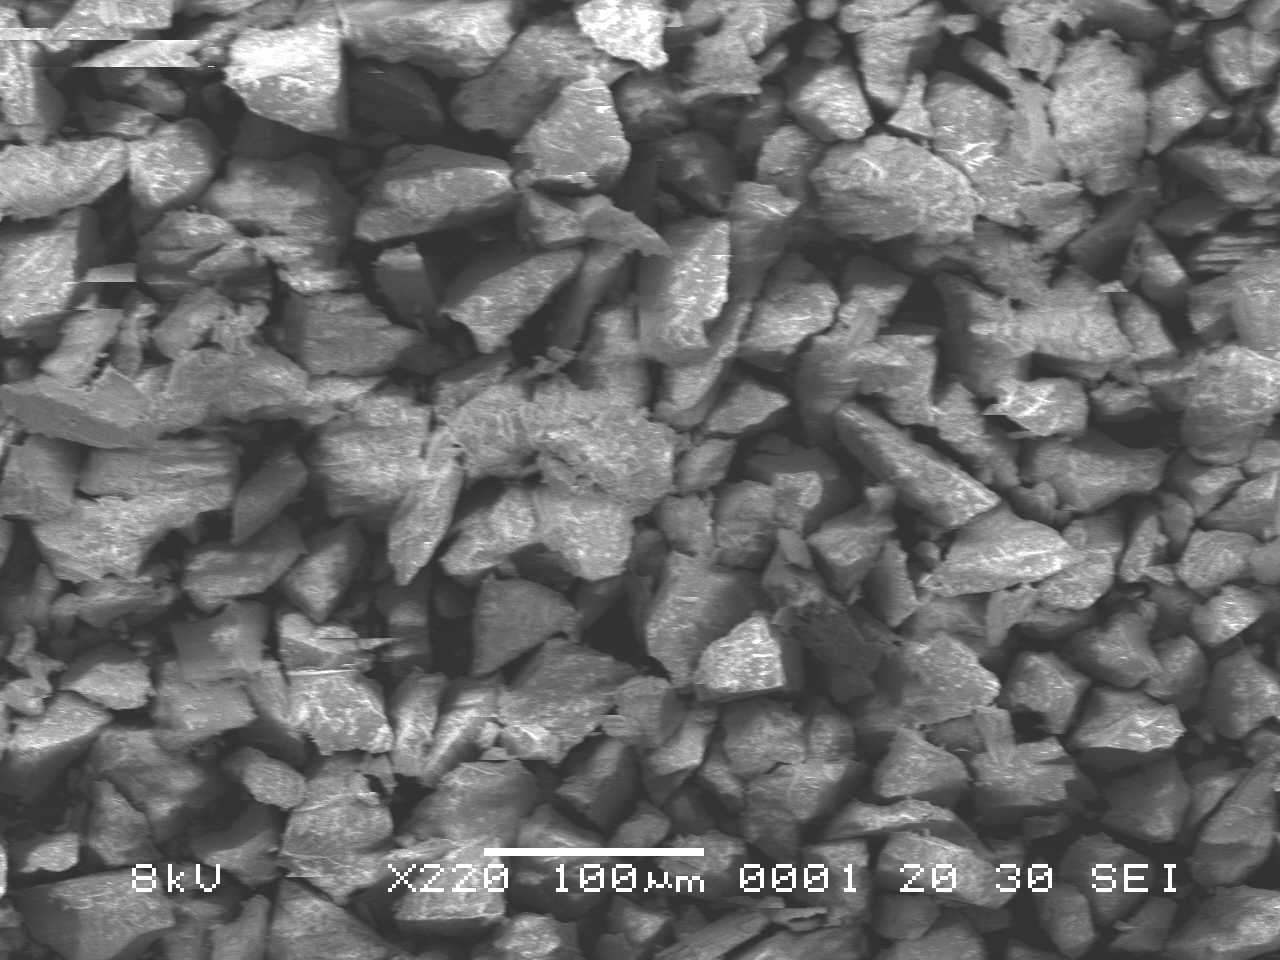
\includegraphics[width=\linewidth]{Az2_x200_2_240221}
\end{minipage}
\caption[SEM images: Sample Az2, azurite]{SEM images: Sample Az2, azurite. Magnification: 200x.}
\label{fig:az2_sem_1}
\end{figure}

In \textit{Figure \ref{fig:az2_sem_2}}, Az2 is shown at 750x (left) and 1500x (right). Imaging at higher magnifications was not possible due to charging. At 750x magnification, relatively flat sides of particles are observed. There is slightly more size variation than initially seen, though this is difficult to assess due to jumping of particles during charging. At 1500x magnification, there is very little surface texture observed. Sample Az2 is obviously unlike the sample HKI natural azurite. However, it also does not resemble known synthetic samples either. 

\begin{figure}[H]
\centering
\begin{minipage}{.45\textwidth}
  \centering
  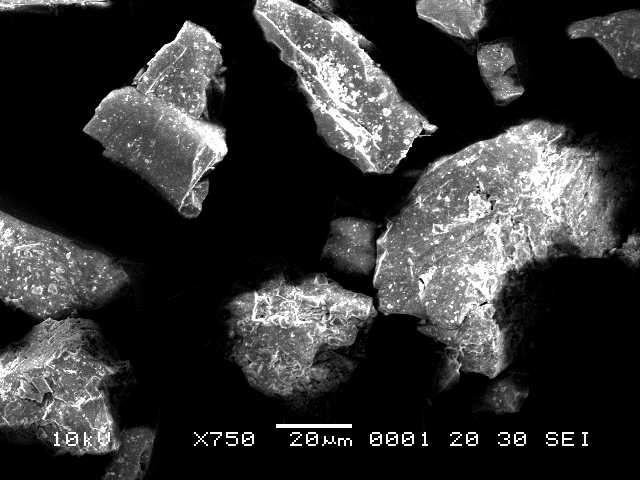
\includegraphics[width=\linewidth]{Az2_x750_1_150321}
\end{minipage}
\begin{minipage}{.45\textwidth}
  \centering
  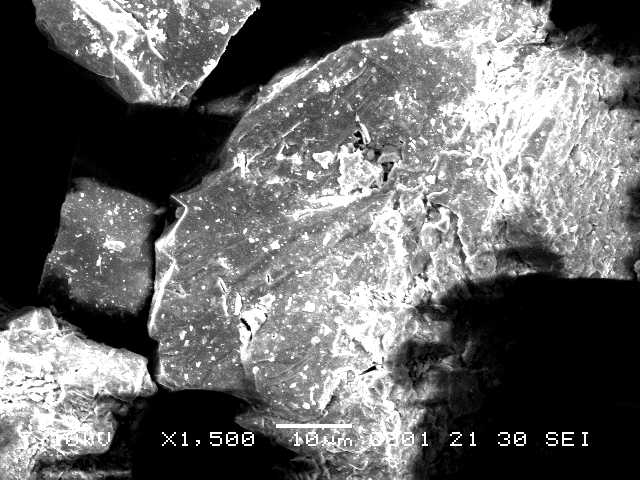
\includegraphics[width=\linewidth]{Az2_x1500_1_150321}
\end{minipage}
\caption[SEM images: Sample Az2, azurite]{SEM images: Sample Az2, azurite. Magnification: \textbf{left)} 750x, \textbf{right)} 1500x}
\label{fig:az2_sem_2}
\end{figure}

% ************************************************     AzMag     *******************************************************************

\textit{Figures \ref{fig:azmag_sem_1}-\ref{fig:azmag_sem_5}} show sample AzMag at magnifications from 200x to 4000x. 

At 200-250x magnification (\textit{Figure \ref{fig:azmag_sem_1}}), extremely small particles are shown. The particle size is fairly homogeneous, though there is a great deal of variation in particle shape as well as a lot of texture observed.

\begin{figure}[H]
\centering
\begin{minipage}{.45\textwidth}
  \centering
  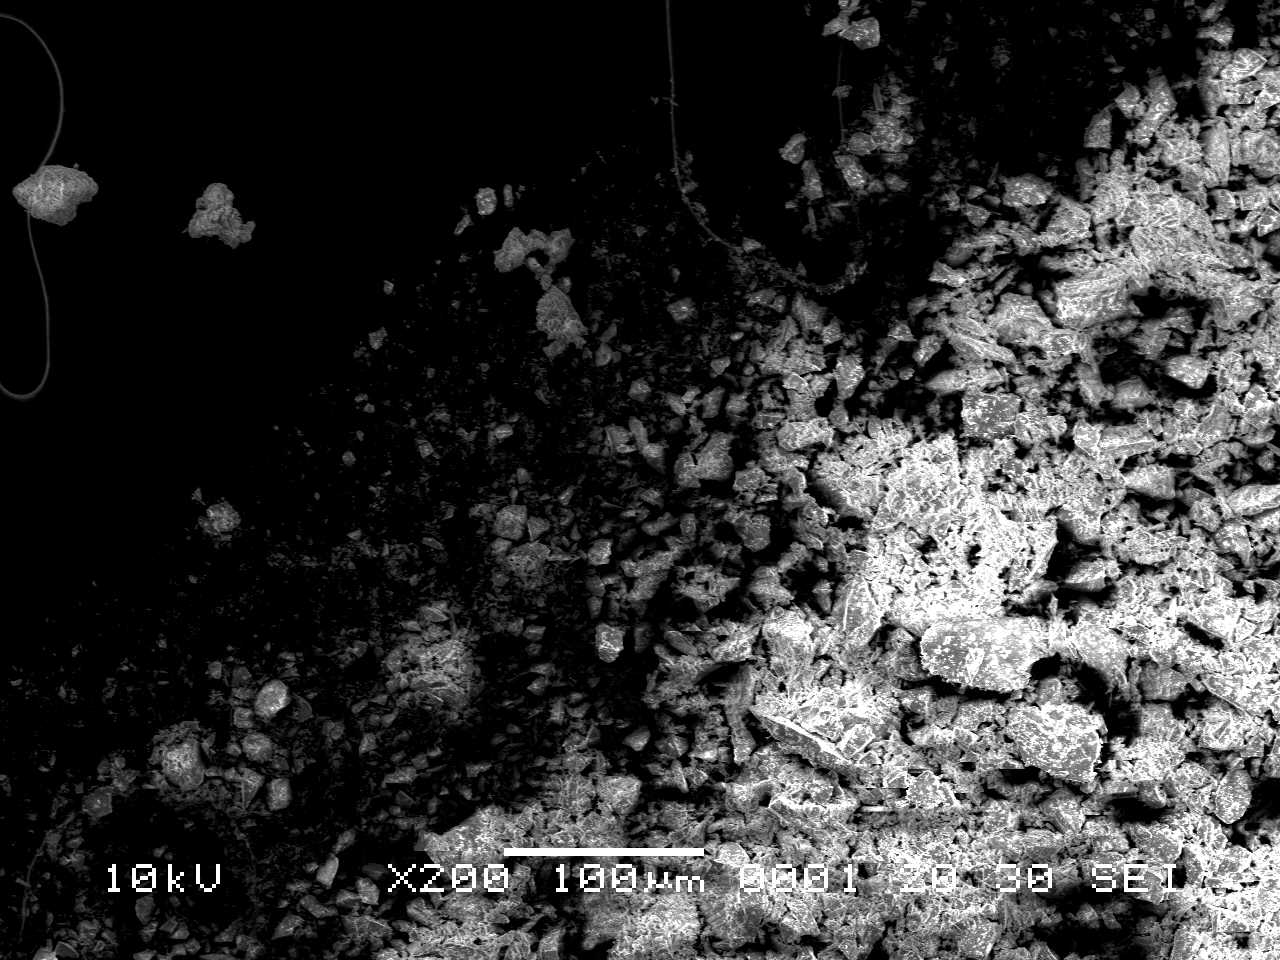
\includegraphics[width=\linewidth]{AzMag_x200_1_260221}
\end{minipage}
\begin{minipage}{.45\textwidth}
  \centering
  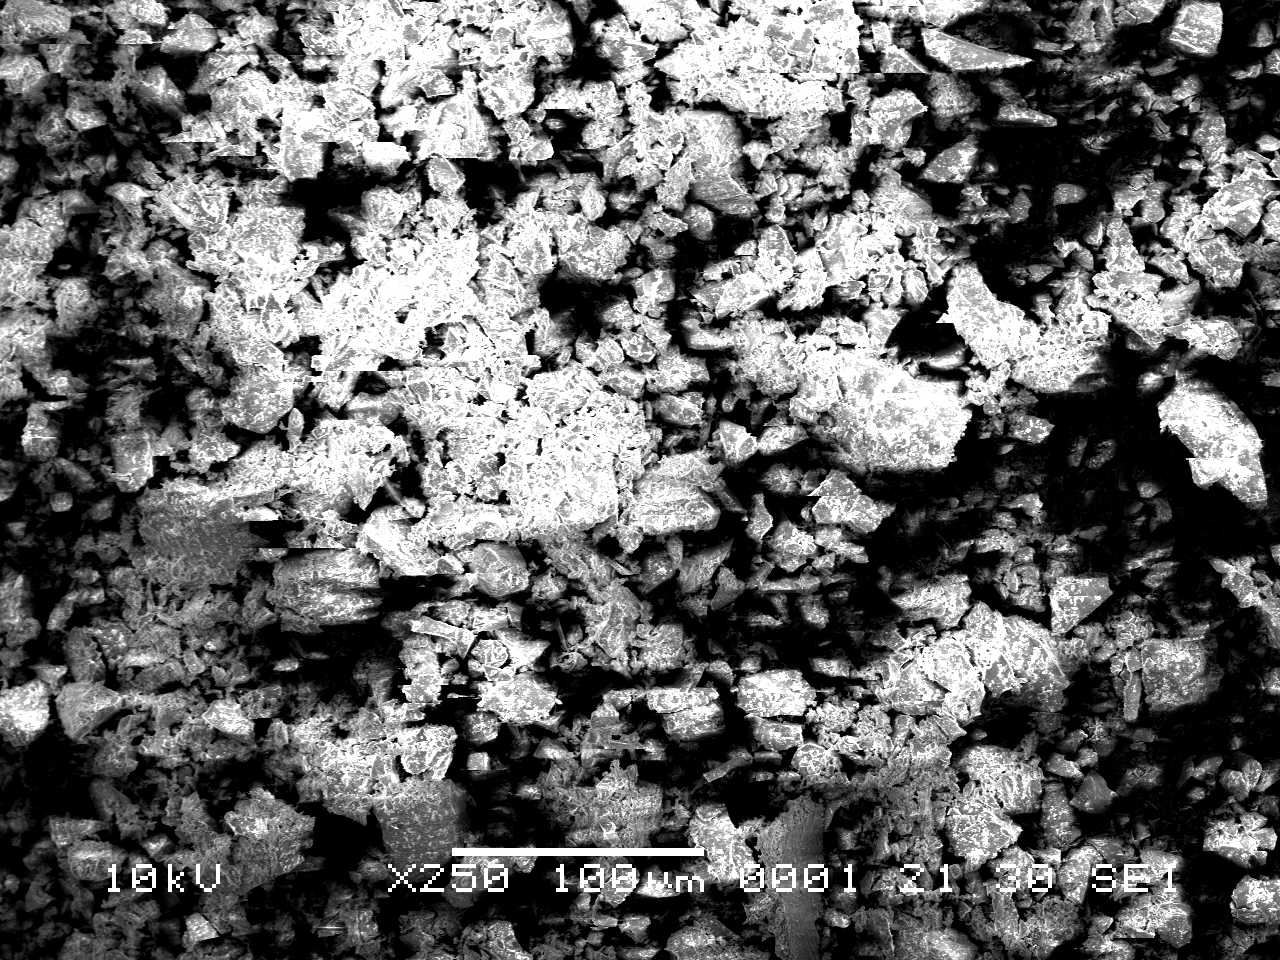
\includegraphics[width=\linewidth]{AzMag_x250_2_160321}
\end{minipage}
\caption[SEM images: Sample AzMag, azurite]{SEM images: Sample AzMag, azurite. Magnification: \textbf{left)} 200x, \textbf{right)} 250x}
\label{fig:azmag_sem_1}
\end{figure}

\textit{Figure \ref{fig:azmag_sem_2}} shows the sample at 750x magnification. The surfaces are choppy, rough, and highly textured. Most particles are approximately square or triangular, with a few small spheres on the surface. Elongated and large particles are not observed.

\begin{figure}[H]
\centering
\begin{minipage}{.45\textwidth}
  \centering
  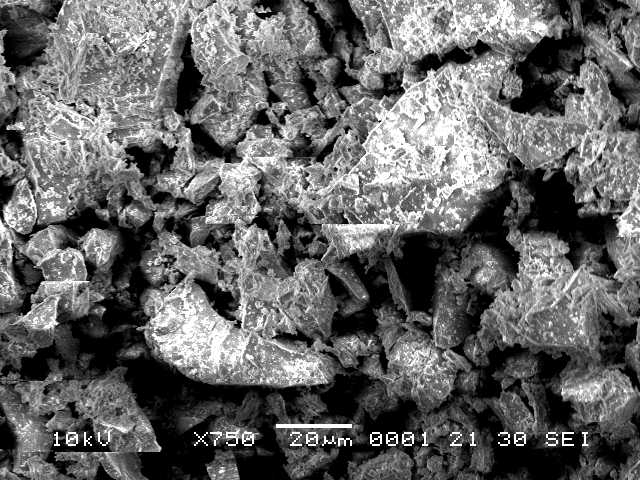
\includegraphics[width=\linewidth]{AzMag_x750_1_160321}
\end{minipage}
\begin{minipage}{.45\textwidth}
  \centering
  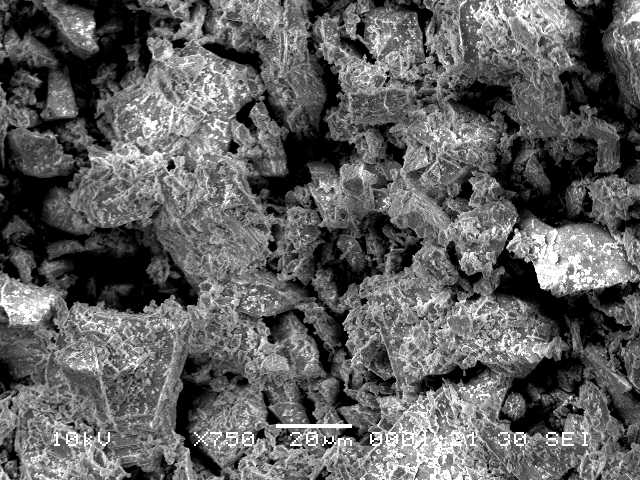
\includegraphics[width=\linewidth]{AzMag_x750_3_160321}
\end{minipage}
\caption[SEM images: Sample AzMag, azurite]{SEM images: Sample AzMag, azurite. Magnification: 750x}
\label{fig:azmag_sem_2}
\end{figure}

\textit{Figure \ref{fig:azmag_sem_3}} and the left image in \textit{Figure \ref{fig:azmag_sem_4}} show the sample at 1500x magnification. Here, sample AzMag is qualitatively similar to HKI natural azurite. There are thinnner forms, though they are not quite as delicate as the needle like formations discussed previously. 

\begin{figure}[H]
\centering
\begin{minipage}{.45\textwidth}
  \centering
  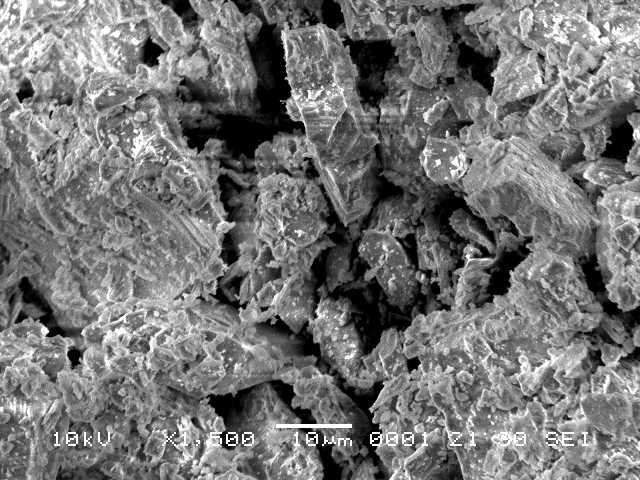
\includegraphics[width=\linewidth]{AzMag_x1500_1_160321}
\end{minipage}
\begin{minipage}{.45\textwidth}
  \centering
  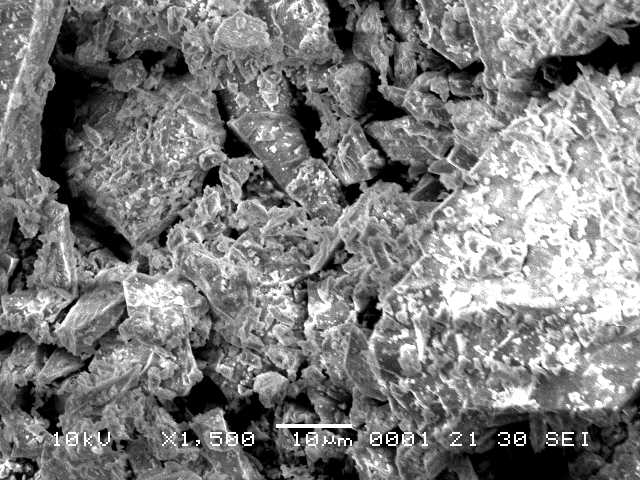
\includegraphics[width=\linewidth]{AzMag_x1500_3_160321}
\end{minipage}
\caption[SEM images: Sample AzMag, azurite]{SEM images: Sample AzMag, azurite. Magnification: 1500x}
\label{fig:azmag_sem_3}
\end{figure}

\begin{figure}[H]
\centering
\begin{minipage}{.45\textwidth}
  \centering
  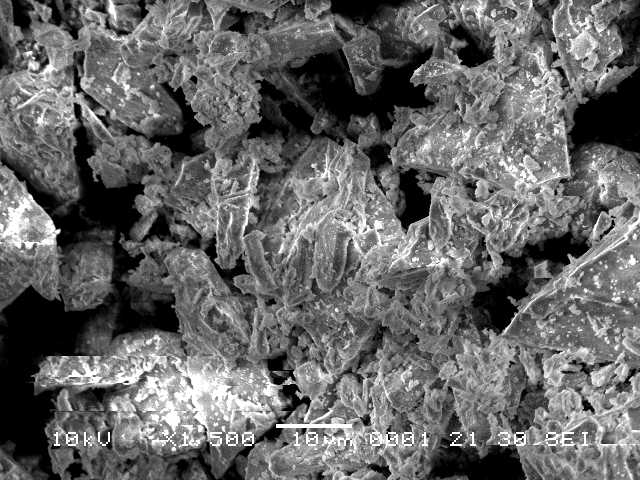
\includegraphics[width=\linewidth]{AzMag_x1500_5_160321}
\end{minipage}
\begin{minipage}{.45\textwidth}
  \centering
  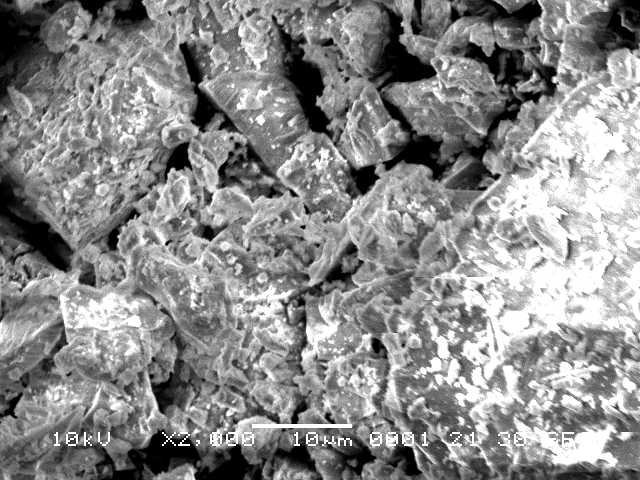
\includegraphics[width=\linewidth]{AzMag_x2000_1_160321}
\end{minipage}
\caption[SEM images: Sample AzMag, azurite]{SEM images: Sample AzMag, azurite. Magnification: \textbf{left)} 1500x, \textbf{right)} 2000x}
\label{fig:azmag_sem_4}
\end{figure}

At high magnification, the surface texture of the sample is clearly visualized. \textit{Figure \ref{fig:azmag_sem_5}} shows elongated, narrow crystals at 3000x (left) and 4000x (right). The directionality observed in HKI natural azurite at high magnifications is not observed here. However, the degree of roughness and character of the surfaces is very similar, implying that this sample is naturally produced.

\begin{figure}[H]
\centering
\begin{minipage}{.45\textwidth}
  \centering
  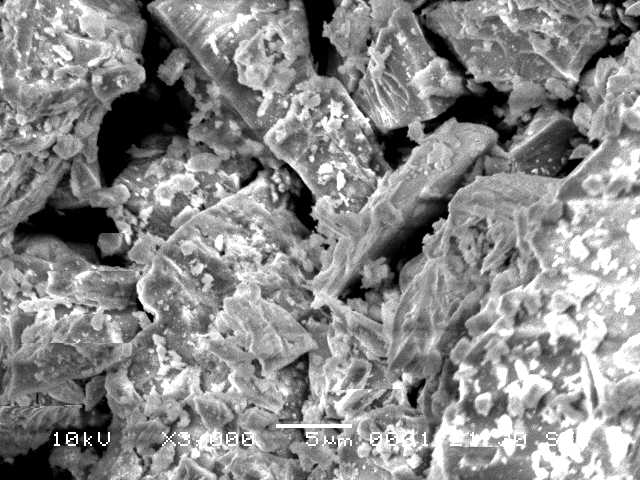
\includegraphics[width=\linewidth]{AzMag_x3000_1_160321}
\end{minipage}
\begin{minipage}{.45\textwidth}
  \centering
  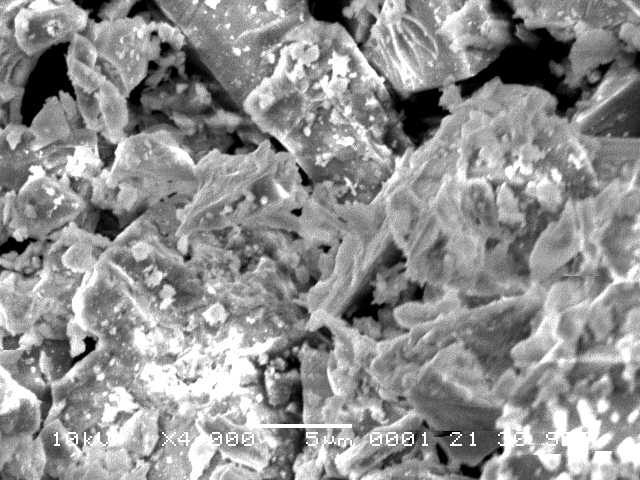
\includegraphics[width=\linewidth]{AzMag_x4000_1_160321}
\end{minipage}
\caption[SEM images: Sample AzMag, azurite]{SEM images: Sample AzMag, azurite. Magnification: \textbf{left)} 3000x, \textbf{right)} 4000x}
\label{fig:azmag_sem_5}
\end{figure}

% ************************************************     AzOp     *******************************************************************

\textit{Figures \ref{fig:azop_sem_1}-\ref{fig:azop_sem_3}} show sample AzOp at magnifications from 250x to 2000x. 

At 250x magnification (\textit{Figure \ref{fig:azop_sem_1}}, left), small and very textured particles are observed. The size of these particles is fairly homogenous. At 750x magnification (\textit{Figure \ref{fig:azop_sem_1}}, right), it is clear that there are larger particles/aggregations. It is difficult to tell whether these are in fact single pieces or clumps of smaller particles. The shape of all particles is extremely asymmetrical and varied, except in one specific case; at the bottom of the image there is a cluster of fairly uniformly spherical particles. 

\begin{figure}[H]
\centering
\begin{minipage}{.45\textwidth}
  \centering
  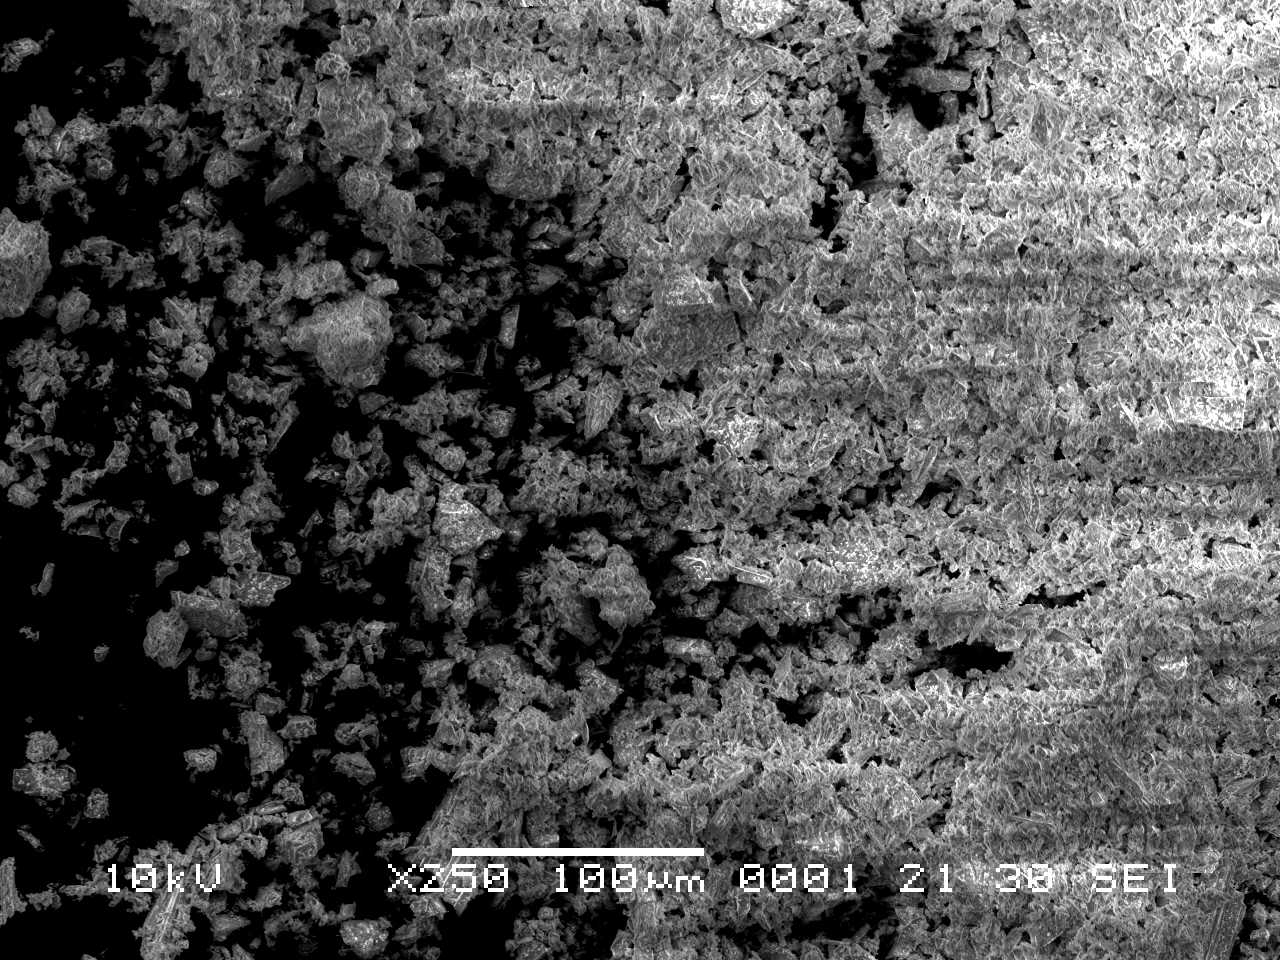
\includegraphics[width=\linewidth]{AzOp_x250_1_150321}
\end{minipage}
\begin{minipage}{.45\textwidth}
  \centering
  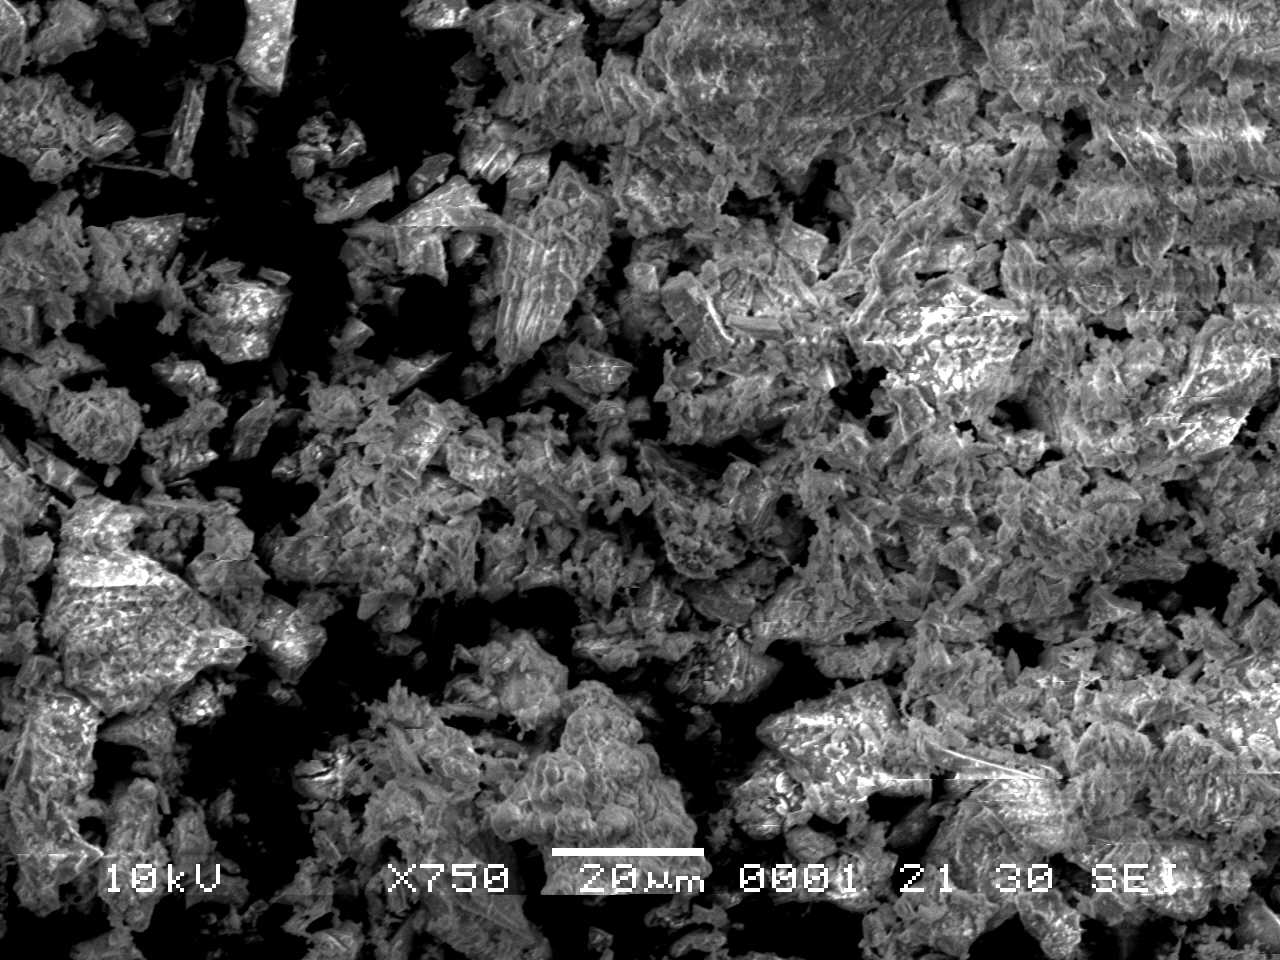
\includegraphics[width=\linewidth]{AzOp_x750_2_150321}
\end{minipage}
\caption[SEM images: Sample AzOp, azurite]{SEM images: Sample AzOp, azurite. Magnification: \textbf{left)} 250x, \textbf{right)} 750x}
\label{fig:azop_sem_1}
\end{figure}

The spherical particles are clearly observed in \textit{Figure \ref{fig:azop_sem_2}}, left, and \textit{Figure \ref{fig:azop_sem_3}}, right. They appear bubbly, as if many partial spheres have formed one on top of the other. This texture is not observed extensively in this sample, nor in other samples such as AzMag and HKI natural azurite that are otherwise similar to the rest of sample AzOp. This could be the result of sample contamination, as several samples were analyzed at the same time, or this could be evidence of multiple conditions under which crystals formed before being mixed to make this pigment. Regardless, this type of morphology is quite uniform and does not look like the result of random crushing and grinding. This certainly must be investigated further by imaging over a larger area of this sample as well as by preparing additional fresh samples.

In contrast, the rougher and more heterogenous texture of the majority of the sample is shown at 2000x magnification in \textit{Figure \ref{fig:azop_sem_3}}, left, and at 4000x magnification in \textit{Figure \ref{fig:azop_sem_2}}, right. Very few remotely circular particles are seen, and there is a great deal of heterogeneity in size and shape. This is very similar to natural samples discussed above.

\begin{figure}[H]
\centering
\begin{minipage}{.45\textwidth}
  \centering
  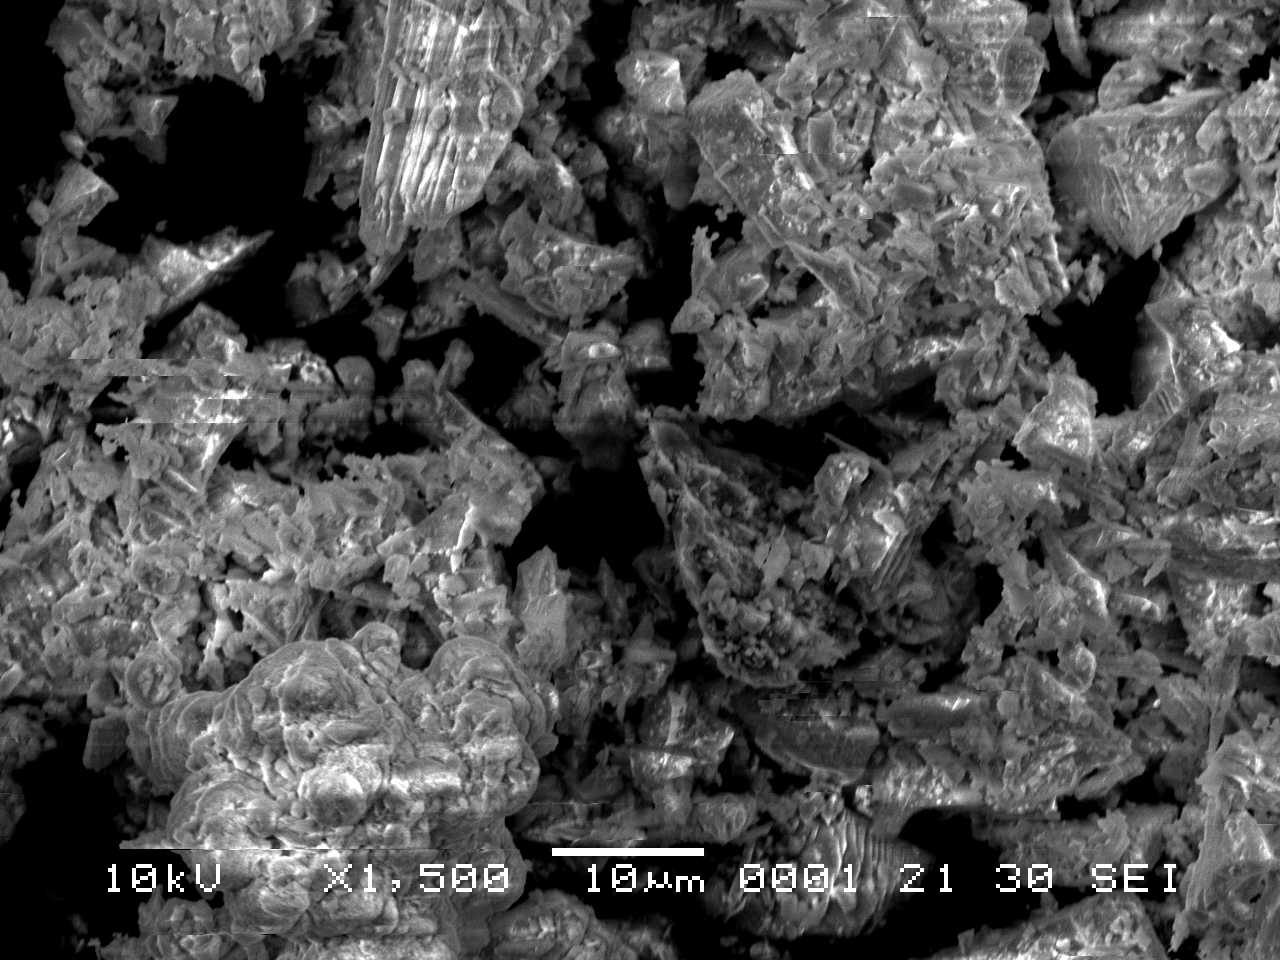
\includegraphics[width=\linewidth]{AzOp_x1500_2_150321}
\end{minipage}
\begin{minipage}{.45\textwidth}
  \centering
  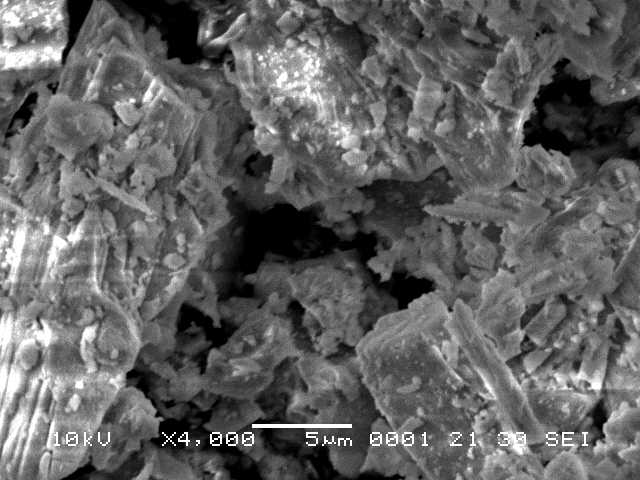
\includegraphics[width=\linewidth]{AzOp_x4000_1_150321}
\end{minipage}
\caption[SEM images: Sample AzOp, azurite]{SEM images: Sample AzOp, azurite. Magnification: \textbf{left)} 1500x, \textbf{right)} 4000x}
\label{fig:azop_sem_2}
\end{figure}

\begin{figure}[H]
\centering
\begin{minipage}{.45\textwidth}
  \centering
  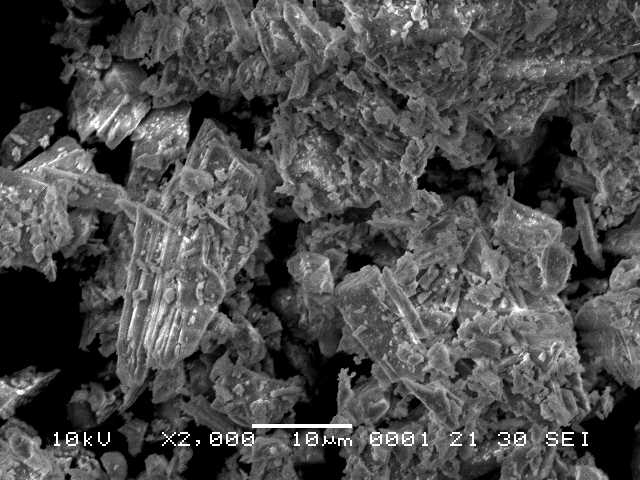
\includegraphics[width=\linewidth]{AzOp_x2000_1_150321}
\end{minipage}
\begin{minipage}{.45\textwidth}
  \centering
  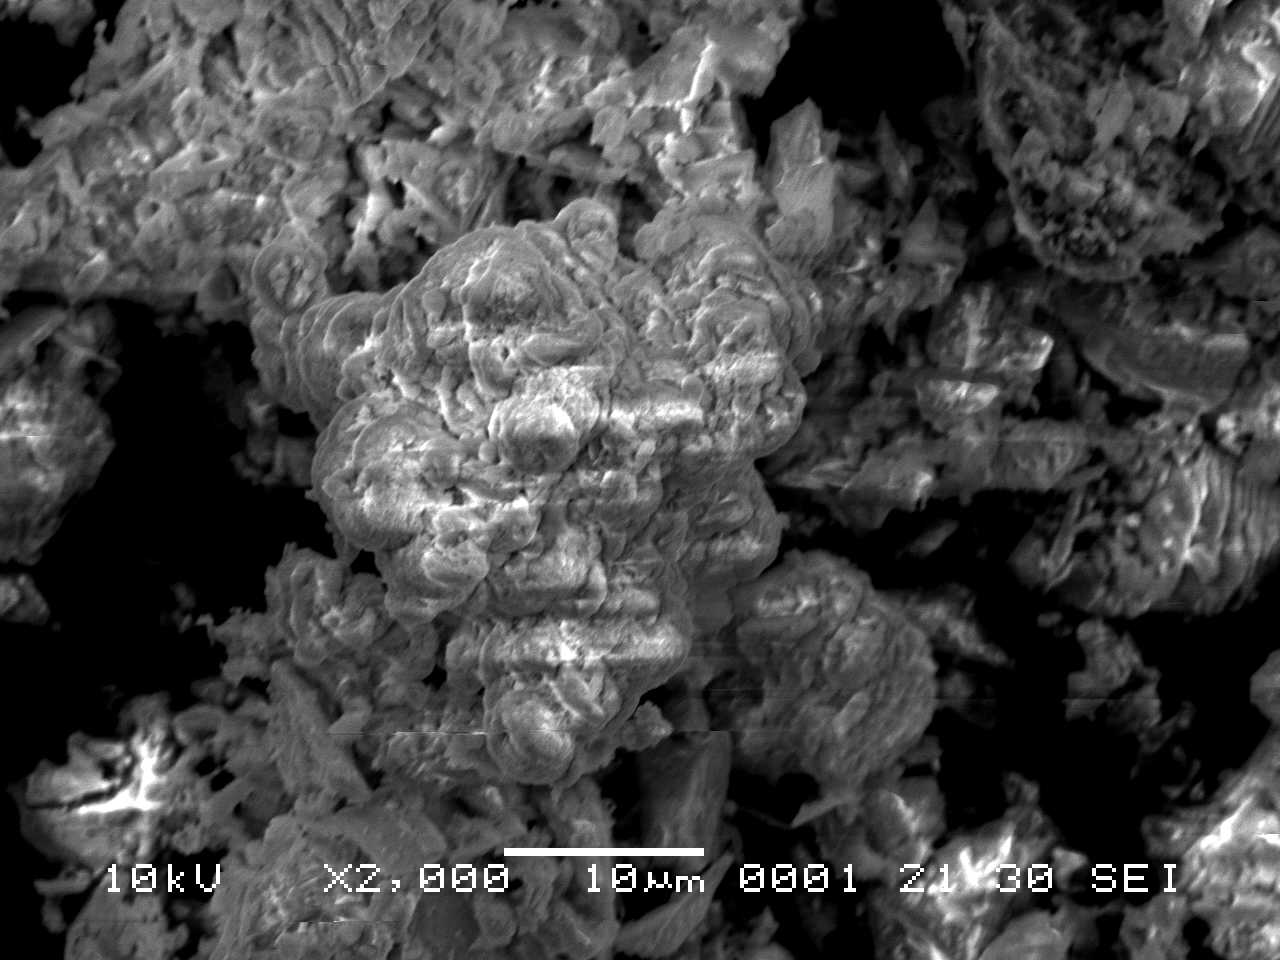
\includegraphics[width=\linewidth]{AzOp_x2000_4_150321}
\end{minipage}
\caption[SEM images: Sample AzOp, azurite]{SEM images: Sample AzOp, azurite. Magnification: 2000x}
\label{fig:azop_sem_3}
\end{figure}

% ************************************************     Fitz1     *******************************************************************
\todo{can you use NLP or ML to do this kind of pattern recognization?? this could be good to look into further.}

\textit{Figures \ref{fig:Fitz1_sem_1}} and \textit{Figure \ref{fig:Fitz1_sem_2}} show sample Fitz1 at magnifications from 250x to 2500x. This sample is described as blue verditer, suggesting that it is synthetic rather than natural.

At 250x magnification (\textit{Figure \ref{fig:Fitz1_sem_1}}, left), small uniform particles are seen. These appear generally circular and far more consistent in size and shape than the samples discussed thus far. At 750x magnification (\textit{Figure \ref{fig:Fitz1_sem_1}}, right), it is possible to qualitatively assess the diameter of particles as consistently < 5 $\mu$m. Particles resemble the spherical cluster observed in the sample AzOp. There is regularity of both size and shape, but it is difficult to determine whether the particles are flat discs or stacked semicircles occupying more volume.

\begin{figure}[H]
\centering
\begin{minipage}{.45\textwidth}
  \centering
  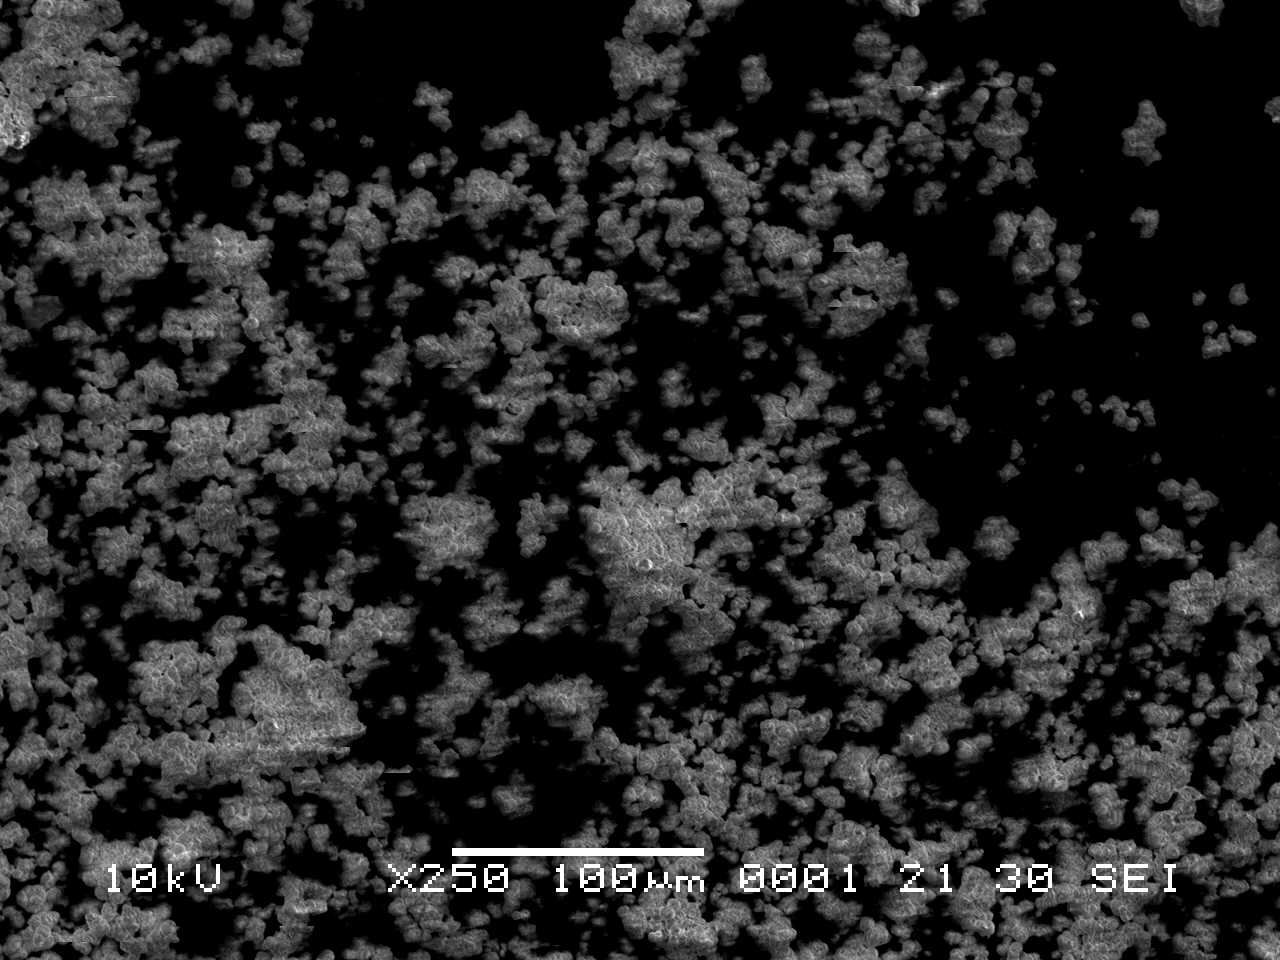
\includegraphics[width=\linewidth]{Fitz1_x250_1_030321}
\end{minipage}
\begin{minipage}{.45\textwidth}
  \centering
  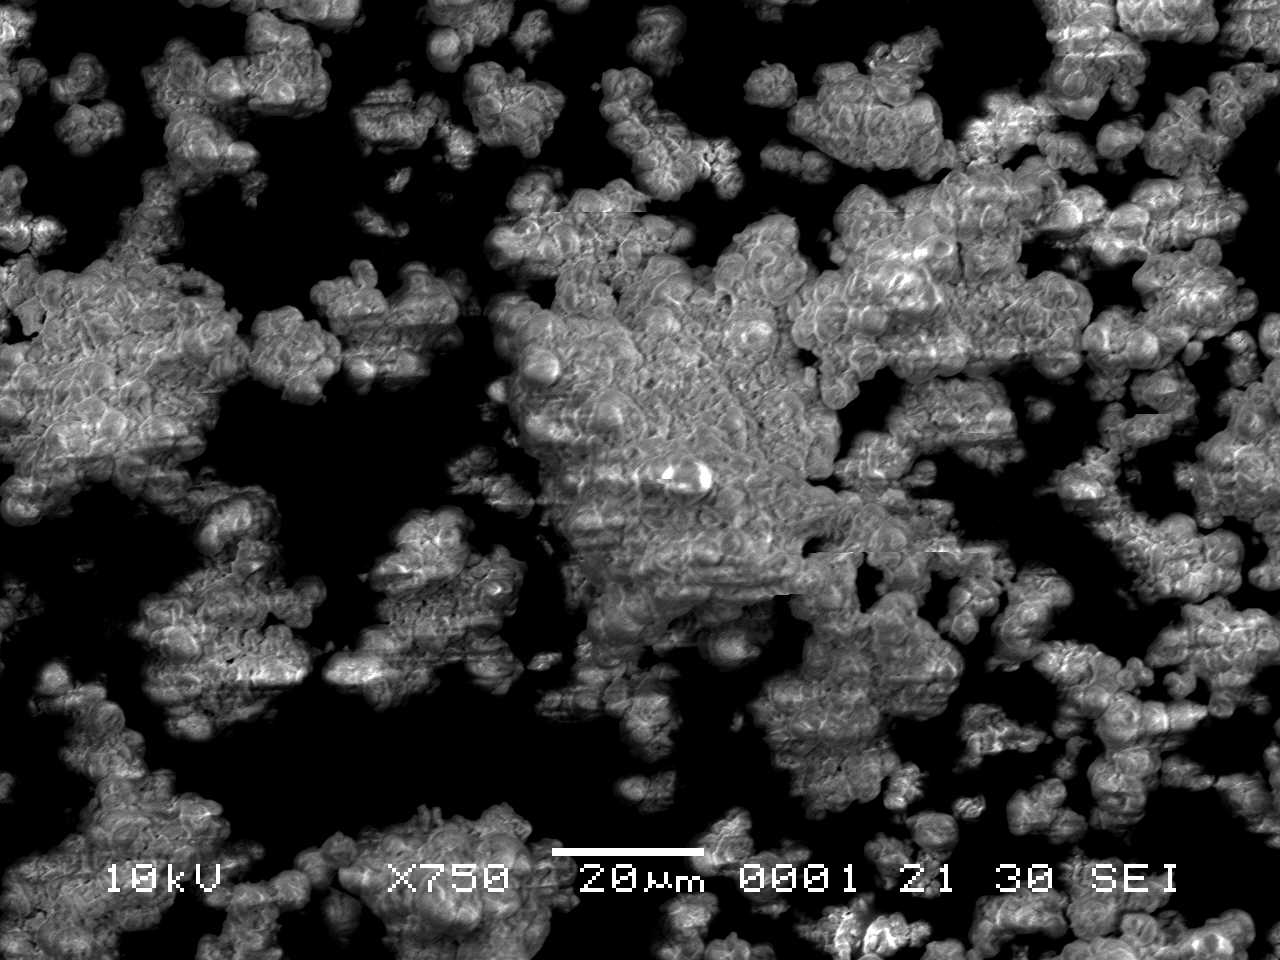
\includegraphics[width=\linewidth]{Fitz1_x750_1_030321}
\end{minipage}
\caption[SEM images: Sample Fitz1, blue verditer]{SEM images: Sample Fitz1, blue verditer. Magnification: \textbf{left)} 250x, \textbf{right)} 750x}
\label{fig:Fitz1_sem_1}
\end{figure}

At 1500x magnification (\textit{Figure \ref{fig:Fitz1_sem_2}}, left), there are clearly spherical particles. These have formed aggregates, though it is not clear whether individual particles could be separated back out of the larger clusters. The size is similar to the spherical cluster in the AzOp sample. The surface also looks slightly pocked or porous. 

The image shown at 2500x magnification (\textit{Figure \ref{fig:Fitz1_sem_2}}, right) is of lower quality than that at 1500x due to surface charging and jumping which made slower acquisitions unsuccessful. The faster acquisition does appear to flatten the image somewhat, which is important to consider since this makes it difficult to judge the volume of particles. There appear to be relatively flat aggregations of approximately circular particles with diameters of approximately 5 $\mu$m.

\begin{figure}[H]
\centering
\begin{minipage}{.45\textwidth}
  \centering
  \includegraphics[width=\linewidth]{Fitz1_x1500_2_030321}
\end{minipage}
\begin{minipage}{.45\textwidth}
  \centering
  \includegraphics[width=\linewidth]{Fitz1_x2500_1_030321}
\end{minipage}
\caption[SEM images: Sample Fitz1, blue verditer]{SEM images: Sample Fitz1, blue verditer. Magnification: \textbf{left)} 1500x, \textbf{right)} 2500x}
\label{fig:Fitz1_sem_2}
\end{figure}

% ************************************************     KE3     *******************************************************************

\textit{Figures \ref{fig:KE3_sem_1}} and \textit{Figure \ref{fig:KE3_sem_2}} show sample KE3 at magnifications from 250x to 2000x. The sample is described as light verditer bice. Verditer suggests a synthetic origin, while bice is used to refer to both natural and synthetic blue pigments. Tentatively, this sample is assumed to be synthetic based on this information.

The image collected at 250x magnification (\textit{Figure \ref{fig:KE3_sem_1}}, left) showed minor issues with charging. Very small particles are present with minimal aggregation. These appear very uniform in size and slightly spherical. At 750x magnification (\textit{Figure \ref{fig:KE3_sem_1}}, right), the uniformity of the particles is more easily observed. They are fairly symmetric, but more angular than sample Fitz1. There are some areas of needle-like structures as well as stacks of spherical or octagonal particles forming small aggregates.

\begin{figure}[H]
\centering
\begin{minipage}{.45\textwidth}
  \centering
  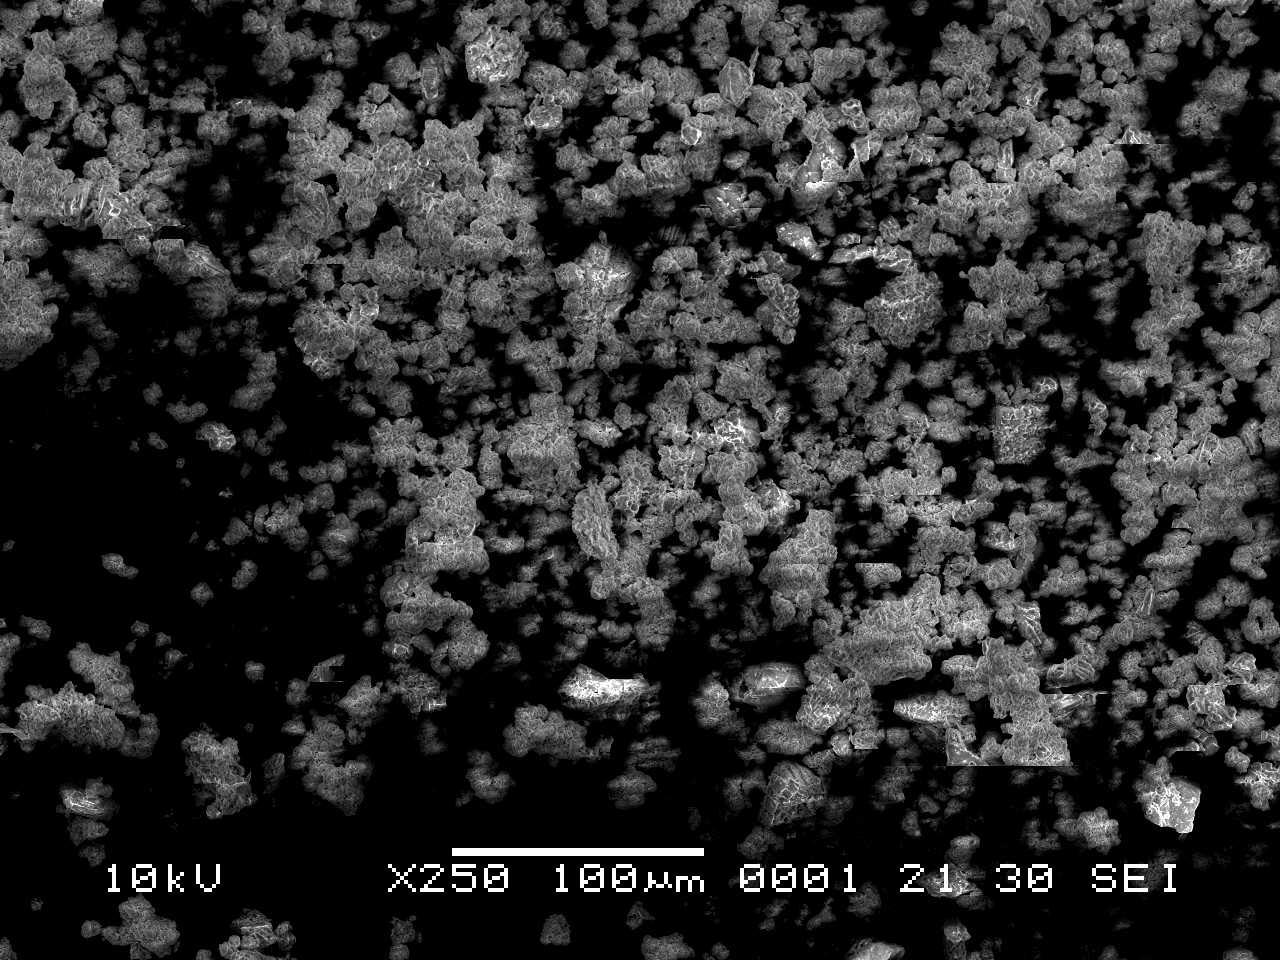
\includegraphics[width=\linewidth]{KE3_x250_1_050321}
\end{minipage}
\begin{minipage}{.45\textwidth}
  \centering
  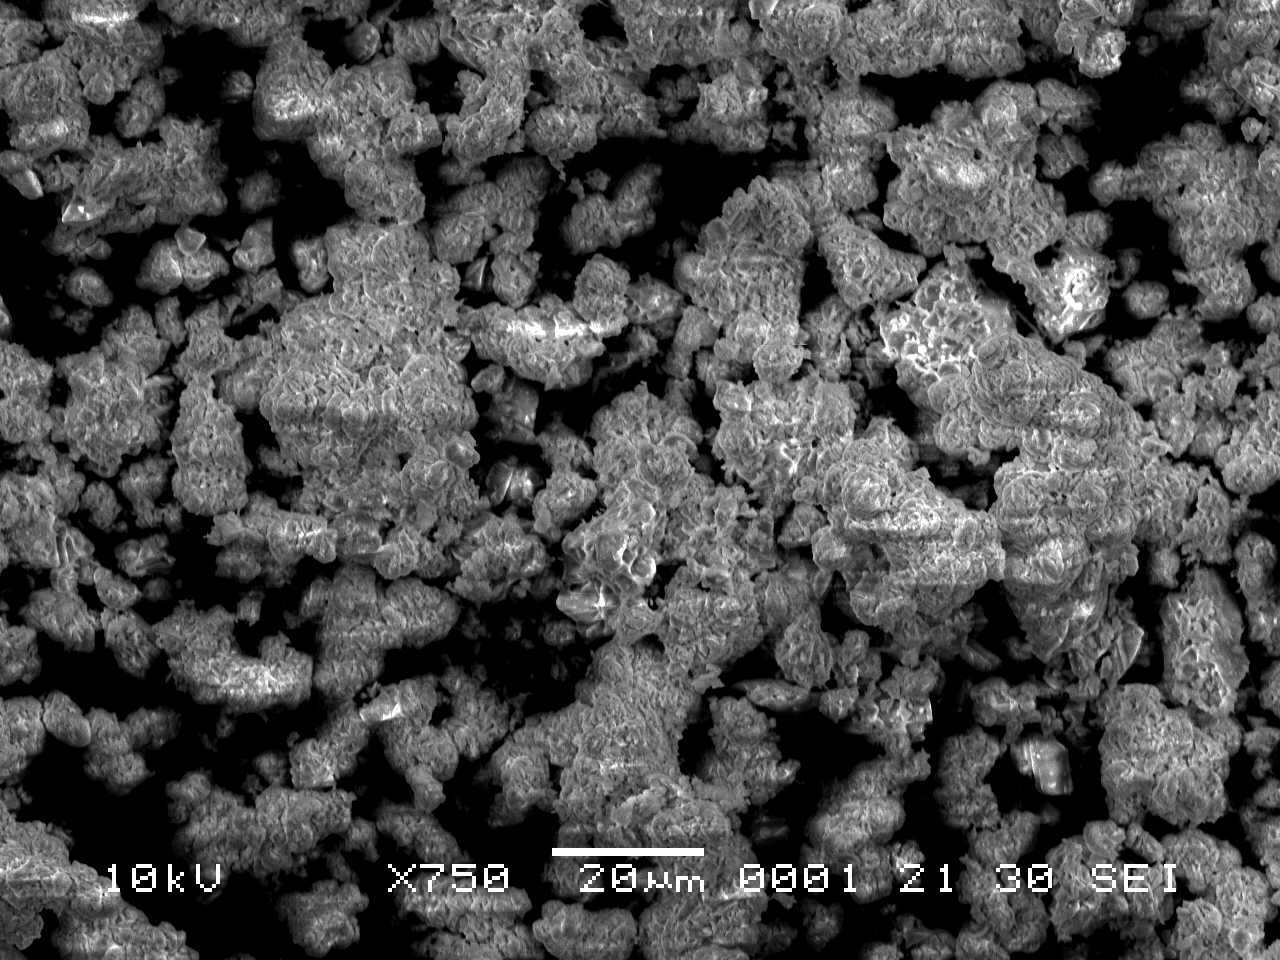
\includegraphics[width=\linewidth]{KE3_x750_3_050321}
\end{minipage}
\caption[SEM images: Sample KE3, light verditer bice]{SEM images: Sample KE3, light verditer bice. Magnification: \textbf{left)} 250x, \textbf{right)} 750x}
\label{fig:KE3_sem_1}
\end{figure}

The approximate particle size can be approximated to 5-10 $\mu$m from the image collected at 1500x magnification (\textit{Figure \ref{fig:KE3_sem_2}}, left). The surfaces appear more porous or pocked than sample Fitz1, but particles are more spherical and uniform than samples from natural origin. At 2000x magnification (\textit{Figure \ref{fig:KE3_sem_2}}, right), spheres are observed. There is significant texture on the surface that is quite fine especially around the edges of particles, and this texture appears rougher than that of sample Fitz1. This may be due, though, to poorer image quality of the Fitz1 sample.

\begin{figure}[H]
\centering
\begin{minipage}{.45\textwidth}
  \centering
  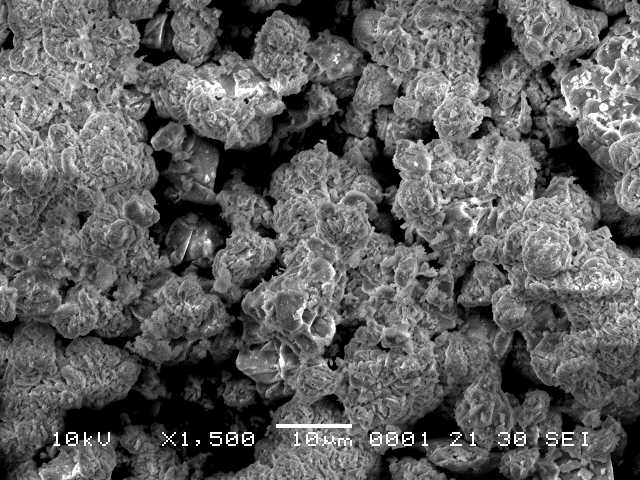
\includegraphics[width=\linewidth]{KE3_x1500_1_050321}
\end{minipage}
\begin{minipage}{.45\textwidth}
  \centering
  \includegraphics[width=\linewidth]{KE3_x2000_2_050321}
\end{minipage}
\caption[SEM images: Sample KE3, light verditer bice]{SEM images: Sample KE3, light verditer bice. Magnification: \textbf{left)} 1500x, \textbf{right)} 2000x}
\label{fig:KE3_sem_2}
\end{figure}

% ************************************************     KE4     *******************************************************************

\textit{Figures \ref{fig:KE4_sem_1}} and \textit{Figure \ref{fig:KE4_sem_2}} show sample KE4 at magnifications from 250x to 2000x. KE4 is labelled as blue bice, which is an ambiguous description, so it is inconclusive whether this sample was prepared naturally or synthetically.

\textit{Figure \ref{fig:KE4_sem_1}} (left) shows KE4 at 250x magnification. Larger particles on the order of 50 $\mu$m are visible, as are significantly smaller particles on the order of 5 $\mu$m. At 750x magnification (\textit{Figure \ref{fig:KE4_sem_1}}, right), fine needle-like structure is visible similar to that of sample HKI natural azurite. At the same time, there are also rounder structures that resemble Fitz1. 

\begin{figure}[H]
\centering
\begin{minipage}{.45\textwidth}
  \centering
  \includegraphics[width=\linewidth]{KE4_x250_1_030321}
\end{minipage}
\begin{minipage}{.45\textwidth}
  \centering
  \includegraphics[width=\linewidth]{KE4_x750_1_030321}
\end{minipage}
\caption[SEM images: Sample KE4, blue bice]{SEM images: Sample KE4, blue bice. Magnification: \textbf{left)} 250x, \textbf{right)} 750x}
\label{fig:KE4_sem_1}
\end{figure}

\textit{Figure \ref{fig:KE4_sem_2}} (left) shows KE4 at 1000x magnification, where the fine structure resembling needles or feathers is very clear. These structures are not oriented in any way, and appear randomly assembled. \textit{Figure \ref{fig:KE4_sem_2}} (right) shows KE4 at 2000x magnification. The image is focused on the flat side of a larger particle (or aggregate) with many smaller particles attached to or resting on the surface. There are also pockmarks or cavities observed. This sample is ambiguous as it shows characteristics of known natural as well as synthetic samples.

\begin{figure}[H]
\centering
\begin{minipage}{.45\textwidth}
  \centering
  \includegraphics[width=\linewidth]{KE4_x1000_1_030321}
\end{minipage}
\begin{minipage}{.45\textwidth}
  \centering
  \includegraphics[width=\linewidth]{KE4_x2000_1_030321}
\end{minipage}
\caption[SEM images: Sample KE4, blue bice]{SEM images: Sample KE4, blue bice. Magnification: \textbf{left)} 1000x, \textbf{right)} 2000x}
\label{fig:KE4_sem_2}
\end{figure}

% ************************************************     KE5     *******************************************************************

\textit{Figures \ref{fig:KE5_sem_1}} and \textit{Figure \ref{fig:KE5_sem_2}} show sample KE5 at magnifications from 250x to 2000x. KE5 is described as blue verditer, strongly suggesting a synthetic origin.

\textit{Figure \ref{fig:KE5_sem_1}} (left) shows KE5 at 250x magnification. Small circular particles of uniform size and shape are observed. \textit{Figure \ref{fig:KE5_sem_1}} (right) shows KE5 at 750x magnification. At this magnification, larger aggregates of approximately 80 $\mu$m are clearly seen to be formed from smaller particles. This is very similar to the appearance of Fitz1 at the same magnification. The appearance also brings to mind the crystal formation of desert rose gypsum, characterized by intersecting flat discs forming circular or semicircular three dimensional structures.%~\autocite{hope_gypsum} 

\textit{Figure \ref{fig:KE5_sem_2}} shows KE5 at 1500x magnification (left) and 2000x magnification (right). The circular character of particles is very clearly observed in these images.

\begin{figure}[H]
\centering
\begin{minipage}{.45\textwidth}
  \centering
  \includegraphics[width=\linewidth]{KE5_x250_2_050321}
\end{minipage}
\begin{minipage}{.45\textwidth}
  \centering
  \includegraphics[width=\linewidth]{KE5_x750_1_050321}
\end{minipage}
\caption[SEM images: Sample KE5, blue verditer]{SEM images: Sample KE5, blue verditer. Magnification: \textbf{left)} 250x, \textbf{right)} 750x}
\label{fig:KE5_sem_1}
\end{figure}

\begin{figure}[H]
\centering
\begin{minipage}{.45\textwidth}
  \centering
  \includegraphics[width=\linewidth]{KE5_x1500_1_050321}
\end{minipage}
\begin{minipage}{.45\textwidth}
  \centering
  \includegraphics[width=\linewidth]{KE5_x2000_2_050321}
\end{minipage}
\caption[SEM images: Sample KE5, blue verditer]{SEM images: Sample KE5, blue verditer. Magnification: \textbf{left)} 1500x, \textbf{right)} 2000x}
\label{fig:KE5_sem_2}
\end{figure}

\subsubsection[Particle size distribution of natural and artificial azurite]{Particle size distribution of natural and artificial azurite}
\label{subsubsection3.1.1.1}

SEM images at 750x magnification were collected from edges of loose pigments samples used for SEM analysis above where particles were most loosely dispersed. The two samples selected, HKI natural azurite and Fitz 1, were selected on the basis of their known sources as well as significantly different morphology. These images were processed in Fiji ImageJ (XXXX version) by increasing contrast and manually thresholding (shown in \textit{Figures \ref{} and \ref{}}) followed by manual selection of maximum lengths and measurement using the image scale bar. 

Five images of Fitz 1 were analyzed, with n(particles) = 102. Five images of HKI natural azurite were analyzed, with n(particles) = 127. There is undoubtedly some bias in selected particles due to the difficulty of defining edges in the images, and this may affect the spread of results. Examples of the original SEM image (left) and the thresholded binary image (right, used for measurements) are shown for Fitz 1 in \textit{Figure \ref{fig:imageJ_fitz1}} and for HKI natural azurite in \textit{Figure \ref{fig:imageJ_hki}}. 

\begin{figure}[H]
\centering
\begin{minipage}{.45\textwidth}
  \centering
  \includegraphics[width=\linewidth]{Fitz1_x750_5_130521}
\end{minipage}
\begin{minipage}{.45\textwidth}
  \centering
  \includegraphics[width=\linewidth]{Fitz1_x750_5_130521_BW}
\end{minipage}
\caption[Particle size analysis: Sample Fitz 1]{Particle size analysis: Sample Fitz 1. \textbf{Left)} original SEM image, \textbf{Right)} thresholded binary image.}
\label{fig:imageJ_fitz1}
\end{figure}

\begin{figure}[H]
\centering
\begin{minipage}{.45\textwidth}
  \centering
  \includegraphics[width=\linewidth]{HKI_natural_azurite_x750_1_130521}
\end{minipage}
\begin{minipage}{.45\textwidth}
  \centering
  \includegraphics[width=\linewidth]{HKI_natural_azurite_x750_1_130521-2_BW}
\end{minipage}
\caption[Particle size analysis: Sample HKI natural azurite]{Particle size analysis: Sample HKI natural azurite. \textbf{Left)} original SEM image, \textbf{Right)} thresholded binary image.}
\label{fig:imageJ_hki}
\end{figure}

The measurements from each sample image were combined and analysed using R (version XXXX) to produce a histogram of the frequency of length measurements (bin size = 1 $\mu$m) for each sample, shown in \textit{Figure \ref{fig:histogram_length}}. Based on the different particle morphologies, it would be reasonable to expect that the particle size distribution would differ between samples. Additionally, the presence of a bimodal distribution in the histogram might indicate the formation of aggregates of a specific size from single particles. 

The length distributions of Fitz 1 and HKI natural azurite do not show significant differences. Both show a high frequency of particles with lengths around 5 $\mu$m, with a low frequency of particles or clusters above 10 $\mu$m. Sample Fitz 1 does appear to have several particles of length around 15 $\mu$m, which is absent in HKI natural azurite. This could suggest that aggregates are forming at more consistent sizes than in sample HKI natural azurite. Overall, though, these two samples are statistically very similar in this analysis. \textit{Table \ref{table:r_stats}} contains descriptive statistics, and it is notable how similar the means and medians are between samples.  

\begin{figure}[H]
\centering
\begin{minipage}{.45\textwidth}
  \centering
  \includegraphics[width=\linewidth]{hist_fitz1}
\end{minipage}
\begin{minipage}{.45\textwidth}
  \centering
  \includegraphics[width=\linewidth]{hist_hki}
\end{minipage}
\caption[Particle size analysis: Sample HKI natural azurite]{Particle size analysis: Sample HKI natural azurite. \textbf{Left)} Fitz 1, \textbf{Right)} HKI natural azurite.}
\label{fig:histogram_length}
\end{figure}

\begin{table}[H]
\caption{Descriptive statistics: Fitz 1, HKI natural azurite}
\centering
\label{table:r_stats}
\begin{tabular}{c c c c}
\toprule
Reference sample & Mean & Median & Range \\
\midrule
HKI natural azurite & 5.437 & 8.583 & 1.177 - 52.176 \\
Fitz 1 & 5.878 & 8.683 & 2.414 - 38.367 \\
\bottomrule
\end{tabular}
\end{table}

%fitz 1
%Median : 5.878  
%Mean   : 8.683
%range 2.414 to 38.367
% hki 
%Median : 5.437  
%Mean   : 8.583
%range 1.177 to 52.176

% *******************************************************************************************************************************
% *******************************************************************************************************************************
% *******************************************************************************************************************************

\subsection[Malachite and green verditer]{Malachite and green verditer}
\label{subsection3.1.2}

% ************************************************     Ma1     *******************************************************************

\textit{Figures \ref{fig:Ma1_sem_1}-\ref{fig:Ma1_sem_4}} show sample Ma1 at magnifications from 250x to 4000x. This sample is natural malachite.

At low magnification (200-250x) as shown in \textit{Figure \ref{fig:Ma1_sem_1}}, the sample appears extremely powdery and fine. The size and shape of particles are extremely irregular in both size and shape. 

\begin{figure}[H]
\centering
\begin{minipage}{.45\textwidth}
  \centering
  \includegraphics[width=\linewidth]{Ma1_x200_1_240221}
\end{minipage}
\begin{minipage}{.45\textwidth}
  \centering
  \includegraphics[width=\linewidth]{Ma1_x250_2_160321}
\end{minipage}
\caption[SEM images: Sample Ma1, malachite]{SEM images: Sample Ma1, malachite. Magnification: \textbf{left)} 200x, \textbf{right)} 250x}
\label{fig:Ma1_sem_1}
\end{figure}

At 750x magnification (\textit{Figure \ref{fig:Ma1_sem_2}}, left), the extreme irregularity of particles is apparent. Particles have extremely rough and choppy edges, and these irregular shapes closely resemble those of natural azurite samples in terms of their roughness and sharpness. There are few aggregates or clumps that are larger than 20 $\mu$m. At 1500x magnification (\textit{Figure \ref{fig:Ma1_sem_2}}, right), the texture of surfaces of the large (approx. 20 $\mu$m) aggregates is observed. It consists of particles of less than 5 $\mu$m across. 
\begin{figure}[H]
\centering
\begin{minipage}{.45\textwidth}
  \centering
  \includegraphics[width=\linewidth]{Ma1_x750_2_160321}
\end{minipage}
\begin{minipage}{.45\textwidth}
  \centering
  \includegraphics[width=\linewidth]{Ma1_x1500_2_160321}
\end{minipage}
\caption[SEM images: Sample Ma1, malachite]{SEM images: Sample Ma1, malachite. Magnification: \textbf{left)} 750x, \textbf{right)} 1500x}
\label{fig:Ma1_sem_2}
\end{figure}

\textit{Figure \ref{fig:Ma1_sem_3}} shows two areas of the sample at 2500x magnification. The sample is disordered and heterogeneous. While it is possible that this is due to grinding the pigment during preparation, \textit{Figure \ref{fig:Ma1_sem_4}} shows further disorder at 3000x and 4000x magnification. Here, many particles under 1 $\mu$m across are present, with extremely uneven borders. These are unambiguously single particles rather than surface roughness on a larger plane.


\begin{figure}[H]
\centering
\begin{minipage}{.45\textwidth}
  \centering
  \includegraphics[width=\linewidth]{Ma1_x2500_2_160321}
\end{minipage}
\begin{minipage}{.45\textwidth}
  \centering
  \includegraphics[width=\linewidth]{Ma1_x2500_3_160321}
\end{minipage}
\caption[SEM images: Sample Ma1, malachite]{SEM images: Sample Ma1, malachite. Magnification: 2500x}
\label{fig:Ma1_sem_3}
\end{figure}

\begin{figure}[H]
\centering
\begin{minipage}{.45\textwidth}
  \centering
  \includegraphics[width=\linewidth]{Ma1_x3000_2_160321}
\end{minipage}
\begin{minipage}{.45\textwidth}
  \centering
  \includegraphics[width=\linewidth]{Ma1_x4000_1_160321}
\end{minipage}
\caption[SEM images: Sample Ma1, malachite]{SEM images: Sample Ma1, malachite. Magnification: \textbf{left)} 3000x, \textbf{right)} 4000x}
\label{fig:Ma1_sem_4}
\end{figure}

% ************************************************     KE1a     *******************************************************************

\textit{Figures \ref{fig:KE1a_sem_1}} shows sample KE1a at magnifications 250x (left) and 750x (right). The name of Ke1a, green bice, is ambiguous and could refer to a natural or an artificial sample.

At 250x magnification, small particles form aggregations of approximately 25-50 $\mu$m. The image at 750x magnification is poor quality, and charging prevented use of higher magnifications. The shapes of particles do appear to be squared-off circles with some degree of uniformity. \mynote{(there may be a better way to say this)} They are not, however, spherical like several of the blue pigment samples discussed above. 

This sample is qualitatively more uniform than sample Ma1, and more spherical, but it is more challenging to draw clear conclusions about morphological differences between natural and synthetic green samples compared to blue. There is a much smaller sample size in the reference samples available, as well as ambiguity in sample source, but this also may just mean that green samples do not show marked morphology changes depending on production process.

\begin{figure}[H]
\centering
\begin{minipage}{.45\textwidth}
  \centering
  \includegraphics[width=\linewidth]{KE1a_x250_1_040321}
\end{minipage}
\begin{minipage}{.45\textwidth}
  \centering
  \includegraphics[width=\linewidth]{KE1a_x750_2_040321}
\end{minipage}
\caption[SEM images: Sample KE1a, green bice]{SEM images: Sample KE1a, green bice. Magnification: \textbf{left)} 250x, \textbf{right)} 750x}
\label{fig:KE1a_sem_1}
\end{figure}

% ************************************************     KE1b     *******************************************************************

%didnt do this one

% ************************************************     KE2     *******************************************************************

\textit{Figures \ref{fig:KE2_sem_1}} and \textit{\ref{fig:KE2_sem_2}} show sample KE2, green verditer. The sample name strongly suggests a synthetic source. 

In \textit{Figure \ref{fig:KE2_sem_1}}, the sample is shown at 250x (left) and 750x (right) magnifications. At 250x magnification, the sample appears fairly uniform in size and shape. It is very finely ground or naturally consists of small crystals and aggregates. At 750x magnification, particles are very irregularly shaped, sharp, and generally not elongated.

\begin{figure}[H]
\centering
\begin{minipage}{.45\textwidth}
  \centering
  \includegraphics[width=\linewidth]{KE2_250_1_040321}
\end{minipage}
\begin{minipage}{.45\textwidth}
  \centering
  \includegraphics[width=\linewidth]{KE2_x750_1_040321}
\end{minipage}
\caption[SEM images: Sample KE2, green verditer]{SEM images: Sample KE2, green verditer. Magnification: \textbf{left)} 250x, \textbf{right)} 750x}
\label{fig:KE2_sem_1}
\end{figure}

In \textit{Figure \ref{fig:KE2_sem_2}}, the sample is shown at 1500x (left) and 2000x (right) magnifications. It is possible to estimate the particle size at approximately 7-10 $\mu$m in the image at 1500x magnification. At 2000x magnification, there is a lack of texture on the surface of individual particles. The edges of particles are extremely feathery, which is observed in other samples discussed in this section as well.

\begin{figure}[H]
\centering
\begin{minipage}{.45\textwidth}
  \centering
  \includegraphics[width=\linewidth]{KE2_x1500_040321}
\end{minipage}
\begin{minipage}{.45\textwidth}
  \centering
  \includegraphics[width=\linewidth]{Ke2_x2000_1_040321}
\end{minipage}
\caption[SEM images: Sample KE2, green verditer]{SEM images: Sample KE2, green verditer. Magnification: \textbf{left)} 1500x, \textbf{right)} 2000x}
\label{fig:KE2_sem_2}
\end{figure}


% *******************************************************************************************************************************
% *******************************************************************************************************************************
% *******************************************************************************************************************************

\section[Raman Data]{Raman Data}
\label{section3.2}



\section[AFM Data]{AFM Data}
\label{section3.3}

%!TEX root = ../thesis.tex
%*******************************************************************************
%****************************** FOURTH Chapter **********************************
%*******************************************************************************
\chapter{Conclusion and further work}

% **************************** Define Graphics Path **************************
\ifpdf
    \graphicspath{{Chapter4/Figs/Raster/}{Chapter4/Figs/PDF/}{Chapter4/Figs/}}
\else
    \graphicspath{{Chapter4/Figs/Vector/}{Chapter4/Figs/}}
\fi

% **************************** Chapter text **************************

\section{Conclusion}
\label{section4.1}

This work consists of two strands of research. First, the capability of using spatially-offset Raman spectroscopy to detect and analyse low concentration lampblack carbon glazes was investigated. Glaze samples were constructed using historically significant materials and procedures and analysed using a defocused confocal Raman system to simulate true SORS. Poor detection of pigments due to very strong absorption of the incident beam and surface damage at laser powers sufficient to generate a Raman signal has led us to conclude that this system, limited by strong absorption in dark pigments, is not suitable for this type of analysis. Work was also done to confirm earlier spatially-offset results on two-layer paint samples. The low SORS effect observed on systems containing CdS/TiO\textsubscript{2} shows that this system is capable of analysing some pigment systems, but is not suitable for analysis of lampblack pigment. While there is interesting further work to be done developing more sensitive SORS systems, we believe this will require development of true spatially-offset detection and that this system may be broadly unsuitable for analysis of carbon-based black pigments.

The need to speed sample preparation for use on the SORS system brought up interesting questions regarding sample ageing and the effects of changing various ageing conditions on the resulting linseed oil chemistry. The oxidation of linseed oil, known to depend on environmental conditions and oil additives, is well studied. However, significant gaps in the literature remain regarding the effects of certain pigments on oxidation rates and surface structure. Lampblack carbon pigment has been minimally studied. After the negative results from SORS experiments, we pivoted to an investigation of the effects of lampblack pigment and ultraviolet light exposure on oxidation of a mixture of linseed oil and mastic resin. This work made use of transmission IR spectroscopy as well as AFM-IR and SFG spectroscopy, novel surface analytic methods that have not been widely applied in conservation science.

Results of this work shows that addition of lampblack pigment does affect the oxidation rate of mastic varnish, resolving the uncertainty raised by existing competing sources. The addition of lampblack pigment slows oxidation by approximately one week in thin films. Exposure to ultraviolet light speeds oxidation significantly but also leads to further reactions not observed under natural conditions within the time period available for this experiment. Interesting domain structures were observed in all samples using AFM, and were affected by the presence of lampblack as well as ultraviolet light exposure, with significant intercalation of domain boundaries into domain centers in samples that were exposed to ultraviolet light. SFG spectroscopy suggests that surface conformational order is affected by the addition of lampblack pigment, a very interesting result that merits further study.

\section{Further work}
\label{section4.2}

This work will be continued to resolve unanswered questions raised by AFM and SFG results. While many studies have addressed the oxidation of linseed oil using bulk analytic techniques such as transmission IR, we propose using the novel surface specific methods of SFG and AFM-IR to determine the chemical significance of the surface domains observed in this work. 

In particular, spatially-resolved SFG spectroscopy would determine whether local conformational order is affect by proximity to lampblack particles and how conformational order changes as films oxidise and form a hardened crosslinked structure. Although we have recently struggled to collect useful spectra using AFM-IR, this issue will be resolved in the future and the resolution this method offers will help characterise the changes in surface chemistry accompanying oxidation and identify the cause of the formation of surface domains that seem to vary depending on oxidation and sample conditions.

The identification of specific oxidation products, particularly of mastic resin, is also of interest. Time of flight Secondary Ion Mass Spectrometry (ToF-SIMS) offers some spatial resolution that would allow the selection of samples for mass spectrum analysis from specific sample regions, and this would allow determination of whether different components are segregating on the surface into domains and oxidising \textit{via} different pathways.  

Finally, further work will also address the question of throughdry, or the depth of penetration of oxidation. Throughdry has posed significant problems for artists and industry, since the formation of an oxidised surface layer under certain conditions prevents diffusion of oxygen deeper into the paint film. Determination of the penetration depth of the ultraviolet light into the sample as well as variable angle attenuated total reflectance (ATR) spectroscopy would be useful in determining the degree and rate of throughdry in different samples. 





\include{Chapter5/chapter5}
%\include{Chapter6/chapter6}
%\include{Chapter7/chapter7}



% ********************************** Back Matter *******************************
% Backmatter should be commented out, if you are using appendices after References
%\backmatter

% ********************************** Bibliography ******************************
\begin{spacing}{0.9}

% To use the conventional natbib style referencing
% Bibliography style previews: http://nodonn.tipido.net/bibstyle.php
% Reference styles: http://sites.stat.psu.edu/~surajit/present/bib.htm

%\bibliographystyle{apalike}
%\bibliographystyle{unsrt} % Use for unsorted references  
%\bibliographystyle{plainnat} % use this to have URLs listed in References
%\cleardoublepage
%\bibliography{References/references} % Path to your References.bib file


% If you would like to use BibLaTeX for your references, pass `custombib' as
% an option in the document class. The location of 'reference.bib' should be
% specified in the preamble.tex file in the custombib section.
% Comment out the lines related to natbib above and uncomment the following line.

\printbibliography[heading=bibintoc, title={References}]


\end{spacing}

% ********************************** Appendices ********************************

\begin{appendices} % Using appendices environment for more functunality

%!TEX root = ../thesis.tex
% ******************************* Thesis Appendix A ****************************
\chapter{How to install \LaTeX} 

\section*{Windows OS}

\subsection*{TeXLive package - full version}
\begin{enumerate}
\item	Download the TeXLive ISO (2.2GB) from\\
\href{https://www.tug.org/texlive/}{https://www.tug.org/texlive/}
\item	Download WinCDEmu (if you don't have a virtual drive) from \\
\href{http://wincdemu.sysprogs.org/download/}
{http://wincdemu.sysprogs.org/download/}
\item	To install Windows CD Emulator follow the instructions at\\
\href{http://wincdemu.sysprogs.org/tutorials/install/}
{http://wincdemu.sysprogs.org/tutorials/install/}
\item	Right click the iso and mount it using the WinCDEmu as shown in \\
\href{http://wincdemu.sysprogs.org/tutorials/mount/}{
http://wincdemu.sysprogs.org/tutorials/mount/}
\item	Open your virtual drive and run setup.pl
\end{enumerate}

or

\subsection*{Basic MikTeX - \TeX~ distribution}
\begin{enumerate}
\item	Download Basic-MiK\TeX (32bit or 64bit) from\\
\href{http://miktex.org/download}{http://miktex.org/download}
\item	Run the installer 
\item	To add a new package go to Start >> All Programs >> MikTex >> Maintenance (Admin) and choose Package Manager
\item	Select or search for packages to install
\end{enumerate}

\subsection*{TexStudio - \TeX~ editor}
\begin{enumerate}
\item	Download TexStudio from\\
\href{http://texstudio.sourceforge.net/\#downloads}
{http://texstudio.sourceforge.net/\#downloads} 
\item	Run the installer
\end{enumerate}

\section*{Mac OS X}
\subsection*{MacTeX - \TeX~ distribution}
\begin{enumerate}
\item	Download the file from\\
\href{https://www.tug.org/mactex/}{https://www.tug.org/mactex/}
\item	Extract and double click to run the installer. It does the entire configuration, sit back and relax.
\end{enumerate}

\subsection*{TexStudio - \TeX~ editor}
\begin{enumerate}
\item	Download TexStudio from\\
\href{http://texstudio.sourceforge.net/\#downloads}
{http://texstudio.sourceforge.net/\#downloads} 
\item	Extract and Start
\end{enumerate}


\section*{Unix/Linux}
\subsection*{TeXLive - \TeX~ distribution}
\subsubsection*{Getting the distribution:}
\begin{enumerate}
\item	TexLive can be downloaded from\\
\href{http://www.tug.org/texlive/acquire-netinstall.html}
{http://www.tug.org/texlive/acquire-netinstall.html}.
\item	TexLive is provided by most operating system you can use (rpm,apt-get or yum) to get TexLive distributions
\end{enumerate}

\subsubsection*{Installation}
\begin{enumerate}
\item	Mount the ISO file in the mnt directory
\begin{verbatim}
mount -t iso9660 -o ro,loop,noauto /your/texlive####.iso /mnt
\end{verbatim}

\item	Install wget on your OS (use rpm, apt-get or yum install)
\item	Run the installer script install-tl.
\begin{verbatim}
	cd /your/download/directory
	./install-tl
\end{verbatim}
\item	Enter command `i' for installation

\item	Post-Installation configuration:\\
\href{http://www.tug.org/texlive/doc/texlive-en/texlive-en.html\#x1-320003.4.1}
{http://www.tug.org/texlive/doc/texlive-en/texlive-en.html\#x1-320003.4.1} 
\item	Set the path for the directory of TexLive binaries in your .bashrc file
\end{enumerate}

\subsubsection*{For 32bit OS}
For Bourne-compatible shells such as bash, and using Intel x86 GNU/Linux and a default directory setup as an example, the file to edit might be \begin{verbatim}
edit $~/.bashrc file and add following lines
PATH=/usr/local/texlive/2011/bin/i386-linux:$PATH; 
export PATH 
MANPATH=/usr/local/texlive/2011/texmf/doc/man:$MANPATH;
export MANPATH 
INFOPATH=/usr/local/texlive/2011/texmf/doc/info:$INFOPATH;
export INFOPATH
\end{verbatim}
\subsubsection*{For 64bit OS}
\begin{verbatim}
edit $~/.bashrc file and add following lines
PATH=/usr/local/texlive/2011/bin/x86_64-linux:$PATH;
export PATH 
MANPATH=/usr/local/texlive/2011/texmf/doc/man:$MANPATH;
export MANPATH 
INFOPATH=/usr/local/texlive/2011/texmf/doc/info:$INFOPATH;
export INFOPATH

\end{verbatim}



%\subsection{Installing directly using Linux packages} 
\subsubsection*{Fedora/RedHat/CentOS:}
\begin{verbatim} 
sudo yum install texlive 
sudo yum install psutils 
\end{verbatim}


\subsubsection*{SUSE:}
\begin{verbatim}
sudo zypper install texlive
\end{verbatim}


\subsubsection*{Debian/Ubuntu:}
\begin{verbatim} 
sudo apt-get install texlive texlive-latex-extra 
sudo apt-get install psutils
\end{verbatim}

%%!TEX root = ../thesis.tex
% ******************************* Thesis Appendix B ********************************

\chapter{Installing the CUED class file}

\LaTeX.cls files can be accessed system-wide when they are placed in the
<texmf>/tex/latex directory, where <texmf> is the root directory of the user’s \TeX installation. On systems that have a local texmf tree (<texmflocal>), which
may be named ``texmf-local'' or ``localtexmf'', it may be advisable to install packages in <texmflocal>, rather than <texmf> as the contents of the former, unlike that of the latter, are preserved after the \LaTeX system is reinstalled and/or upgraded.

It is recommended that the user create a subdirectory <texmf>/tex/latex/CUED for all CUED related \LaTeX class and package files. On some \LaTeX systems, the directory look-up tables will need to be refreshed after making additions or deletions to the system files. For \TeX Live systems this is accomplished via executing ``texhash'' as root. MIK\TeX users can run ``initexmf -u'' to accomplish the same thing.

Users not willing or able to install the files system-wide can install them in their personal directories, but will then have to provide the path (full or relative) in addition to the filename when referring to them in \LaTeX.



\end{appendices}

% *************************************** Index ********************************
\printthesisindex % If index is present

\end{document}
